\documentclass[10.5pt,a4paper]{article} 
\usepackage[utf8]{inputenc} 
\usepackage{helvet}
\renewcommand\familydefault{\sfdefault} 
\usepackage[T1]{fontenc}
\usepackage[light]{merriweather} 
%\usepackage{ulem}
\usepackage{setspace} 
\usepackage[hang]{footmisc} 
\renewcommand{\footnotesize}{\scriptsize} 
\usepackage[hyphens]{url}\urlstyle{same} 
\usepackage[colorlinks = true,
            linkcolor = black,
            urlcolor  = blue,
            citecolor = black,
            anchorcolor = black]{hyperref}
% e-mail
\usepackage{etoolbox}
\makeatletter
\newcommand\myemail[3]{%                %\newcommand\tpj@compose@mailto[3]{%
\edef\@tempa{mailto:#1?subject=#2 }%
\edef\@tempb{\expandafter\html@spaces\@tempa\@empty}%
\href{\@tempb}{#3}}
\catcode\%=11
\def\html@spaces#1 #2{#1%20\ifx#2\@empty\else\expandafter\html@spaces\fi#2}
\catcode\%=14
\makeatother
% Colour
\usepackage[svgnames]{xcolor}
\definecolor{rstudio}{HTML}{4b84b7}
\definecolor{cloud}{HTML}{e4eef8}
\newcommand{\rcode}[1]{\texttt{\color{rstudio} #1}}

\Urlmuskip=0mu plus 1mu\relax 
\usepackage[
  ansiapaper,
  margin=0.7in]{geometry}
\usepackage{fancyhdr} % Required for modifying headers and footers
\fancyhead[L]{} % Top left header
\fancyhead[R]{} % Top right header
\renewcommand{\headrulewidth}{1.4pt} % Rule under the header
\fancyfoot[C]{\textbf{\thepage}} % Bottom center footer
\renewcommand{\footrulewidth}{1.4pt} % Rule under the footer
\pagestyle{fancy} % Use the custom headers and footers throughout the document


\usepackage{lipsum,afterpage}
\usepackage{dirtytalk} 
\usepackage{longtable}
\usepackage{adjustbox}
\usepackage{apacite}
\usepackage{natbib}
\usepackage{tkz-euclide}
\usetikzlibrary{calc}
\usepackage{pgfplots}
\pgfplotsset{compat=1.11}
\usepackage {parskip}
\usepackage{epigraph}
\usepackage{graphicx}
\graphicspath{ {images/} }
\pagenumbering{arabic} 
\usepackage{ntheorem}
\newtheorem{hyp}{Hypothesis}
\newtheorem{subhyp}{Hypothesis}[hyp]
\renewcommand\thesubhyp{\thehyp.\alph{subhyp}}
\usepackage{caption}
\usepackage{subcaption}
\usepackage{float}
\usepackage[bf,sf]{titlesec}
\usepackage{microtype}

\renewcommand{\refname}{Bibliography}
\setcounter{secnumdepth}{4}

\titleformat{\paragraph}
{\normalfont\normalsize\bfseries}{\theparagraph}{1em}{}
\titlespacing*{\paragraph}
{0pt}{3.25ex plus 1ex minus .2ex}{1.5ex plus .2ex}

\usepackage[autostyle]{csquotes}
\usepackage{enumitem} % to remove vspace for itemize with [noitemsep]

\usepackage{listings}
\lstset{language=R,
    basicstyle=\small\ttfamily,
    stringstyle=\color{DarkGreen},
    otherkeywords={!,!=,~,$,*,\&,\%/\%,\%*\%,\%\%,<-,<<-,_,/},
    morekeywords={TRUE,FALSE},
    deletekeywords={data,frame,length,as,character},
    keywordstyle=\color{Chocolate},
    commentstyle=\color{DarkSlateGrey},
    literate=%
    {à}{{\`a}}1
    {â}{{\^a}}1
    {è}{{\`e}}1
    {é}{{\'e}}1
    {ê}{{\^e}}1
    {ë}{{\"e}}1
    {ô}{{\^o}}1
    {ù}{{\`u}}1
    {ç}{{\c{c}}}1
    {À}{{\`A}}1
    {Â}{{\^A}}1
    {È}{{\`E}}1
    {É}{{\'E}}1
    {Ê}{{\^E}}1
    {Ë}{{\"E}}1
    {Ô}{{\^O}}1
    {Ù}{{\`U}}1
    {Ç}{{\c{C}}}1
}

\usepackage{xparse}
\ExplSyntaxOn

\usepackage{wrapfig}

\makeatletter
\NewDocumentCommand{\multicitep}{m}
 {
  \NAT@open
  \mjb_multicitep:n { #1 }
  \NAT@close
 }
\makeatother
\seq_new:N \l_mjb_multicite_in_seq
\seq_new:N \l_mjb_multicite_out_seq
\seq_new:N \l_mjb_cite_seq

\cs_new_protected:Npn \mjb_multicitep:n #1
 {
  \seq_set_split:Nnn \l_mjb_multicite_in_seq { ; } { #1 }
  \seq_clear:N \l_mjb_multicite_out_seq
  \seq_map_inline:Nn \l_mjb_multicite_in_seq
   {
    \mjb_cite_process:n { ##1 }
   }
  \seq_use:Nn \l_mjb_multicite_out_seq { ;~ }
 }

\cs_new_protected:Npn \mjb_cite_process:n #1
 {
  \seq_set_split:Nnn \l_mjb_cite_seq { , } { #1 }
  \int_compare:nTF { \seq_count:N \l_mjb_cite_seq == 1 }
   {
    \seq_put_right:Nn \l_mjb_multicite_out_seq
     { \citeauthor{#1},~\citeyear{#1} }
   }
   {
    \seq_put_right:Nx \l_mjb_multicite_out_seq
     {
      \exp_not:N \citeauthor{\seq_item:Nn \l_mjb_cite_seq { 1 }},~
      \exp_not:N \citeyear{\seq_item:Nn \l_mjb_cite_seq { 1 }},~
      \seq_item:Nn \l_mjb_cite_seq { 2 }
     }
   }
 }
\ExplSyntaxOff

\renewcommand{\contentsname}{Table des matières}

\title{\textbf{\emph{RStudio Cloud}} pour les nuls}
\author{William Poirier, Université Laval}
\date{POL-2000}

\begin{document} 

% ----------------------------------------------------------------
\begin{titlepage}
\newgeometry{left=7.5cm} %defines the geometry for the titlepage
\pagecolor{rstudio}
\noindent

\includegraphics[width=14.2cm]{_graphs/cloud.jpg}\\[-1em]
\color{cloud}
\makebox[0pt][l]{\rule{1.4\textwidth}{2pt}}
\par
\noindent
\color{white}
\textbf{Université Laval}
\vfill
\noindent
{\huge\textbf{\emph{RStudio Cloud}} pour les nuls}
\vskip\baselineskip
\noindent
POL-2000, Méthodologie quantitative
\end{titlepage}
\restoregeometry % restores the geometry
\nopagecolor% Use this to restore the color pages to white
% ----------------------------------------------------------------

\tableofcontents

\pagebreak

\section{C'est quoi R?}
Bonjour et bienvenue dans le cours POL-2000! Ce tutoriel sera votre guide de démarrage ainsi qu'un document de référence tout au long du cours\footnote{Tutoriel basé sur le travail de Vincent Arel-Bundock, Yannick Dufresne, et Florence Vallée-Dubois}. Dans l'objectif d'introduire les étudiants de sciences politiques aux méthodes quantitatives et à l'analyse causale en sciences sociales, nous avons cru bon de vous initier au langage de programmation R. N'ayez crainte, c'est plus simple qu'il n'y paraît et vous en tirerez beaucoup d'avantages. 

Pour la petite histoire, la première version de \textbf{R} a été publiée en 1995 par Ross Ihaka et Robert Gentleman, mais le langage s'inspire des travaux de John Chambers aux laboratoires Bell dans les années 1970. Aujourd'hui, \textbf{R} est un outil d'analyse statistique populaire, tant dans le secteur privé que dans le monde universitaire. \textbf{R} est\ ce que l'on appelle un \textit{logiciel libre}, ce qui signifie que son code source est ouvert. Ceci permet à des utilisateurs bénévoles de développer des \textit{packages} (micrologiciel ou librairie de fonctions) qui sont ensuite rendus disponibles à la communauté (pour la plupart gratuitement). Ceci fait de \textbf{R} un outil puissant, flexible, public, et donc particulièrement adapté à la méthode scientifique. 

Le reste du document vous permettra de vous familiariser avec \textbf{R} et avec son environnement de travail. Nous encourageons donc sa lecture attentive.

\section{R vs. RStudio vs. RStudio Cloud}\label{R vs RStudio vs RStudio Cloud}

Une distinction importante à effectuer est la différence entre le langage \textbf{R} et l'\textit{IDE}\footnote{\emph{Integrated development environment} ou environnement de développement intégré.} \textbf{RStudio}. L'\textit{IDE} a pour fonction principale de recevoir le code et de le compiler. En d'autres mots, \textbf{R} c'est la langue que l'on écrit et le papier c'est l'\textit{IDE}. Plusieurs \textit{IDE} existent et il est facile de se perdre dans leurs différents paramètres et fonctionnalités. C'est pourquoi nous imposons l'utilisation de \textbf{RStudio} ou, à proprement parler, de \textbf{RStudio Cloud}. \textbf{RStudio Cloud} est une reproduction de l'environnement \textbf{RStudio} en ligne. De cette façon, tous les étudiants ont accès au même environnement de travail, peu importe l'ordinateur utilisé.  

Ainsi, dans le cadre du cours, les étudiants utiliseront le langage de programmation \textbf{R} à partir de l'environnement \textbf{RStudio Cloud}. Cette distinction s'affinera au cours de la session, n'ayez crainte. Pour les plus curieux d'entre vous, de nombreuses ressources, francophones et anglophones, existent sur internet :

\begin{itemize}
  \item \href{https://stackoverflow.com}{Stackoverflow}
    \begin{itemize}
      \item Google est le meilleur ami des programmeurs. Si vous rencontrez un problème, Google vous fournira sans doute la solution sous la forme d'un \textit{post} sur Stackoverflow. Il s'agit d'un site répertoriant les questions d'utilisateurs concernant la plupart des langages de programmation, incluant \textbf{R}. À la manière du logiciel libre, ce sont les autres utilisateurs du site qui se chargent de répondre avec grande précision. C'est vraiment un outil important. 
    \end{itemize}
  \item \href{https://www.r-bloggers.com}{r-bloggers}
    \begin{itemize}
      \item Pour être informé sur les nouveaux développements de \textbf{R} et de RStudio. Encore une fois, il s'agit d'un point de rencontre de la communauté.
    \end{itemize}
  \item \href{https://www.coursera.org}{Coursera}
    \begin{itemize}
      \item Site de formation en ligne. Les cours ont le format de cours universitaires, mais avec la version gratuite: pas besoin de suivre l’entièreté des plans de cours (ni de remettre les travaux).
    \end{itemize}
  \item \href{https://www.datacamp.com}{DataCamp}
    \begin{itemize}
      \item Similaire à Coursera, DataCamp se concentre sur des exercices pratiques en \textbf{Python}, \textbf{R} et \textbf{SQL}. Avec une approche très pratique, c'est un bon moyen d'accélérer l'intégration de connaissances techniques. 
    \end{itemize}
\item \href{https://www.datanovia.com/en/}{Datanovia}
    \begin{itemize}
      \item Sous forme de tutoriel et de blogue, Datanovia est une excellente source d'information bilingue, spécialement lorsqu'il s'agit de visualisation de données.
    \end{itemize}
\end{itemize}

\section{RStudio Cloud -- La base}
  \subsection{Connexion}
  Dans le cadre du cours, nous utiliserons un espace de travail commun. Pour y accéder, veuillez d'abord vous créer un compte \textbf{RStudio Cloud} en cliquant \href{https://login.rstudio.cloud/register?redirect=https\%3A\%2F\%2Fclient.login.rstudio.cloud\%2Foauth\%2Flogin\%3Fshow_auth\%3D0\%26show_login\%3D0\%26show_setup\%3D0}{\textbf{ici}}. \textbf{N'oubliez pas de vous servir de votre courriel institutionnel (@ulaval.ca) pour ce faire}. Ce lien vous mènera à une page semblable à la figure \ref{login}. Une fois votre compte créé, cliquez \href{https://can01.safelinks.protection.outlook.com/?url=https\%3A\%2F\%2Flogin.rstudio.cloud\%2Finvite\%3Fspace_name\%3DPOL\%2B2000-Z\%2BM\%25C3\%25A9thodes\%2Bquantitatives\%26code\%3D9tltN\%252ByVLqitCL1rVgCB\%252F\%252B0V8rk0Wtqxp\%252Fl6uW8J&amp;data=04\%7C01\%7Cwilliam.poirier.1\%40ulaval.ca\%7C9119a0b3a3fa4119007208d987439312\%7C56778bd56a3f4bd3a26593163e4d5bfe\%7C1\%7C0\%7C637689547430424200\%7CUnknown\%7CTWFpbGZsb3d8eyJWIjoiMC4wLjAwMDAiLCJQIjoiV2luMzIiLCJBTiI6Ik1haWwiLCJXVCI6Mn0\%3D\%7C0&amp;sdata=EMbletbv2\%2Bu9\%2FKSqkqJbRadybcaee2t2S2\%2F8MNRvJgQ\%3D&amp;reserved=0}{\textbf{ici}} pour accéder à l'environnement du cours. Si vous cliquez sur l’hyperlien dans le Portail du cours, vous accèderez à une page semblable à la figure \ref{workspace}, mais les étapes sont les mêmes. Ce lien vous permettra d'accéder à tous les exercices et devoirs du cours qui se servent du logiciel R.
  
\begin{figure}[H]
\centering
\begin{subfigure}{.5\textwidth}
  \centering
  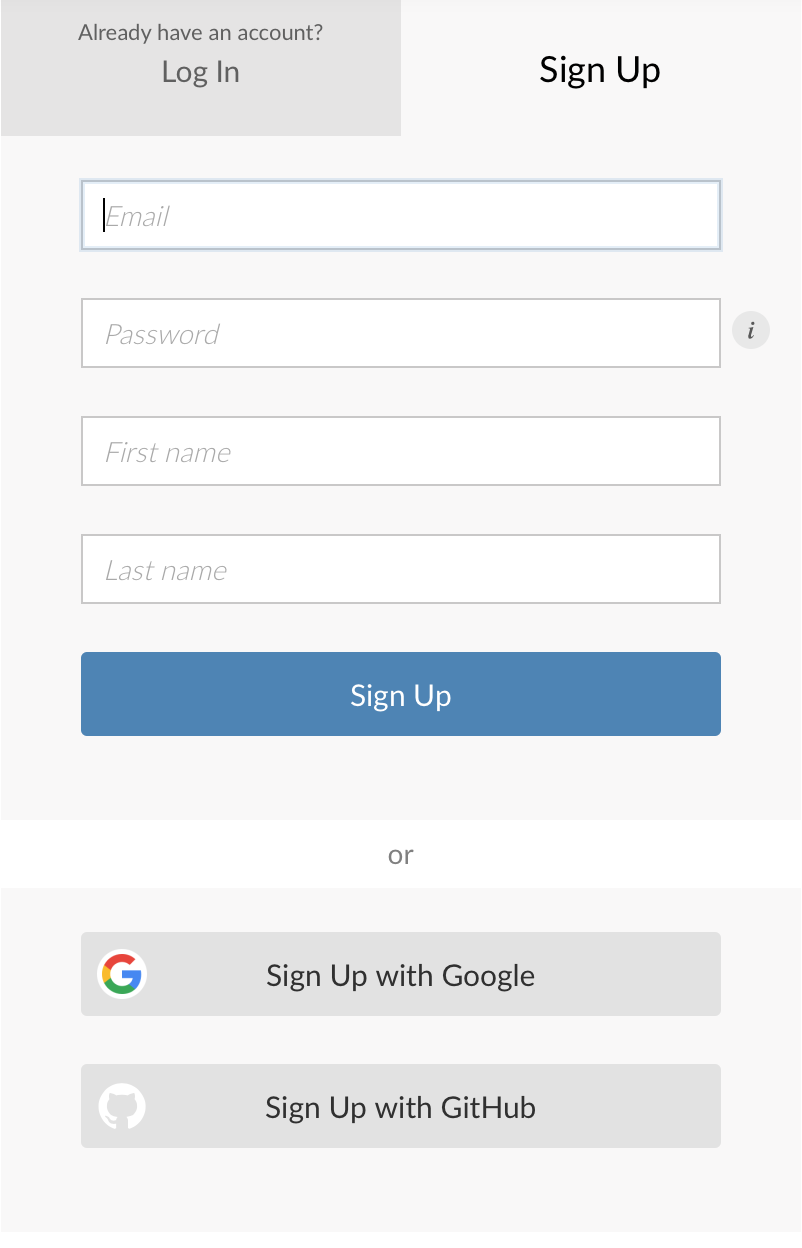
\includegraphics[width=1\linewidth]{_graphs/login.png}
  \caption{Création du compte}
  \label{login}
\end{subfigure}%
\begin{subfigure}{.5\textwidth}
  \centering
  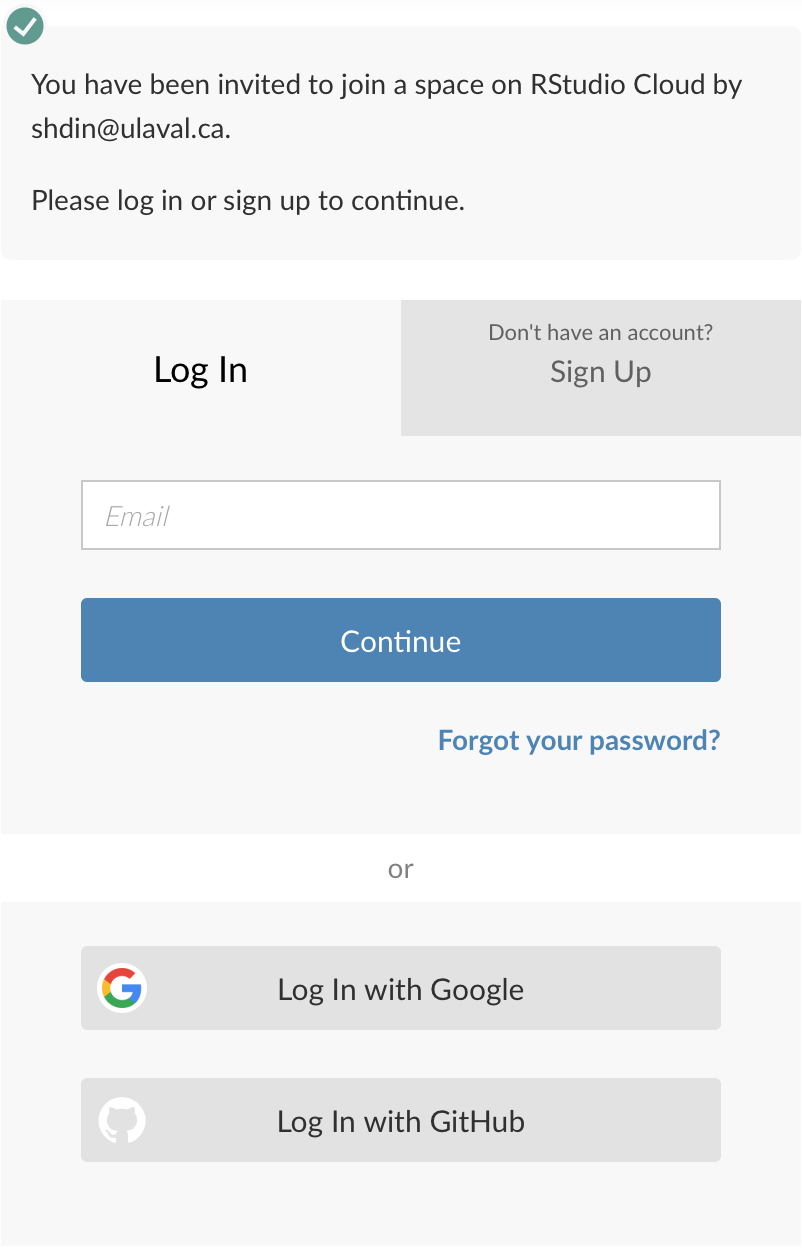
\includegraphics[width=1\linewidth]{_graphs/workspace.png}
  \caption{Inscription à l'environnement}
  \label{workspace}
\end{subfigure}
\caption{Connexion à \textbf{RStudio Cloud}}
\label{connexion}
\end{figure}
  
\begin{figure}[H]
  \centering
  \fbox{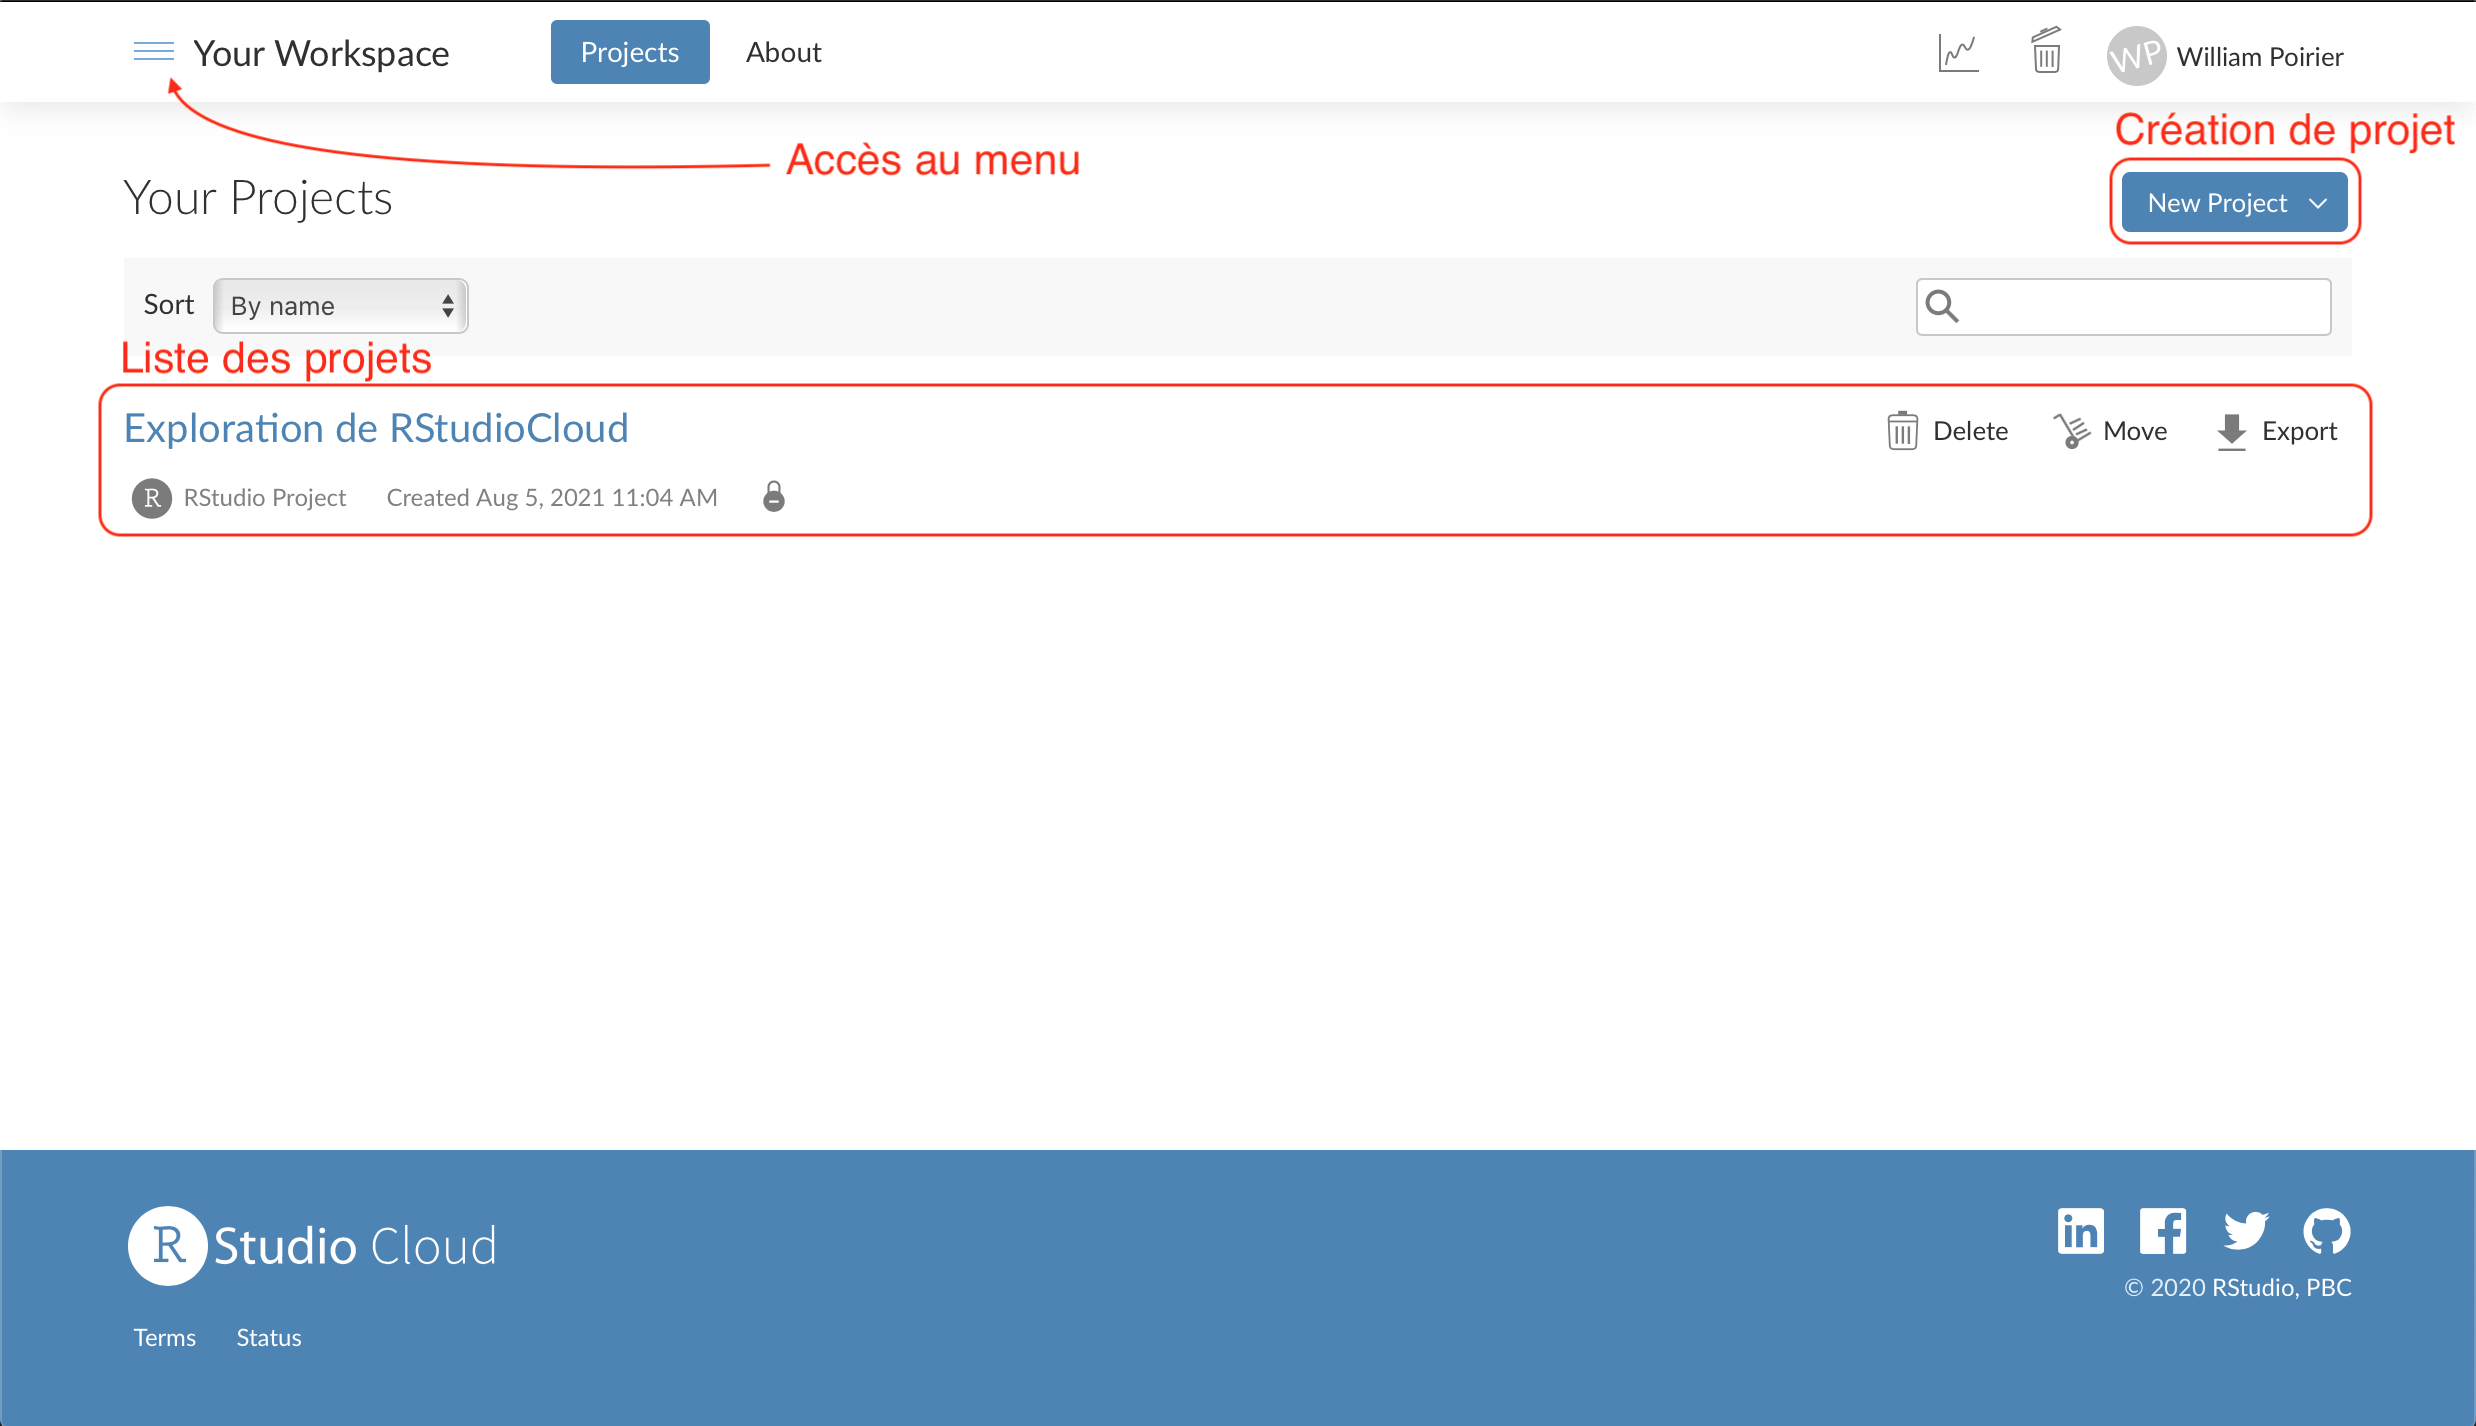
\includegraphics[width=1\linewidth]{_graphs/firstpage.png}}
  \caption{Page d'accueil}
  \label{home}
\end{figure}

\begin{figure}[H]
  \centering
  \fbox{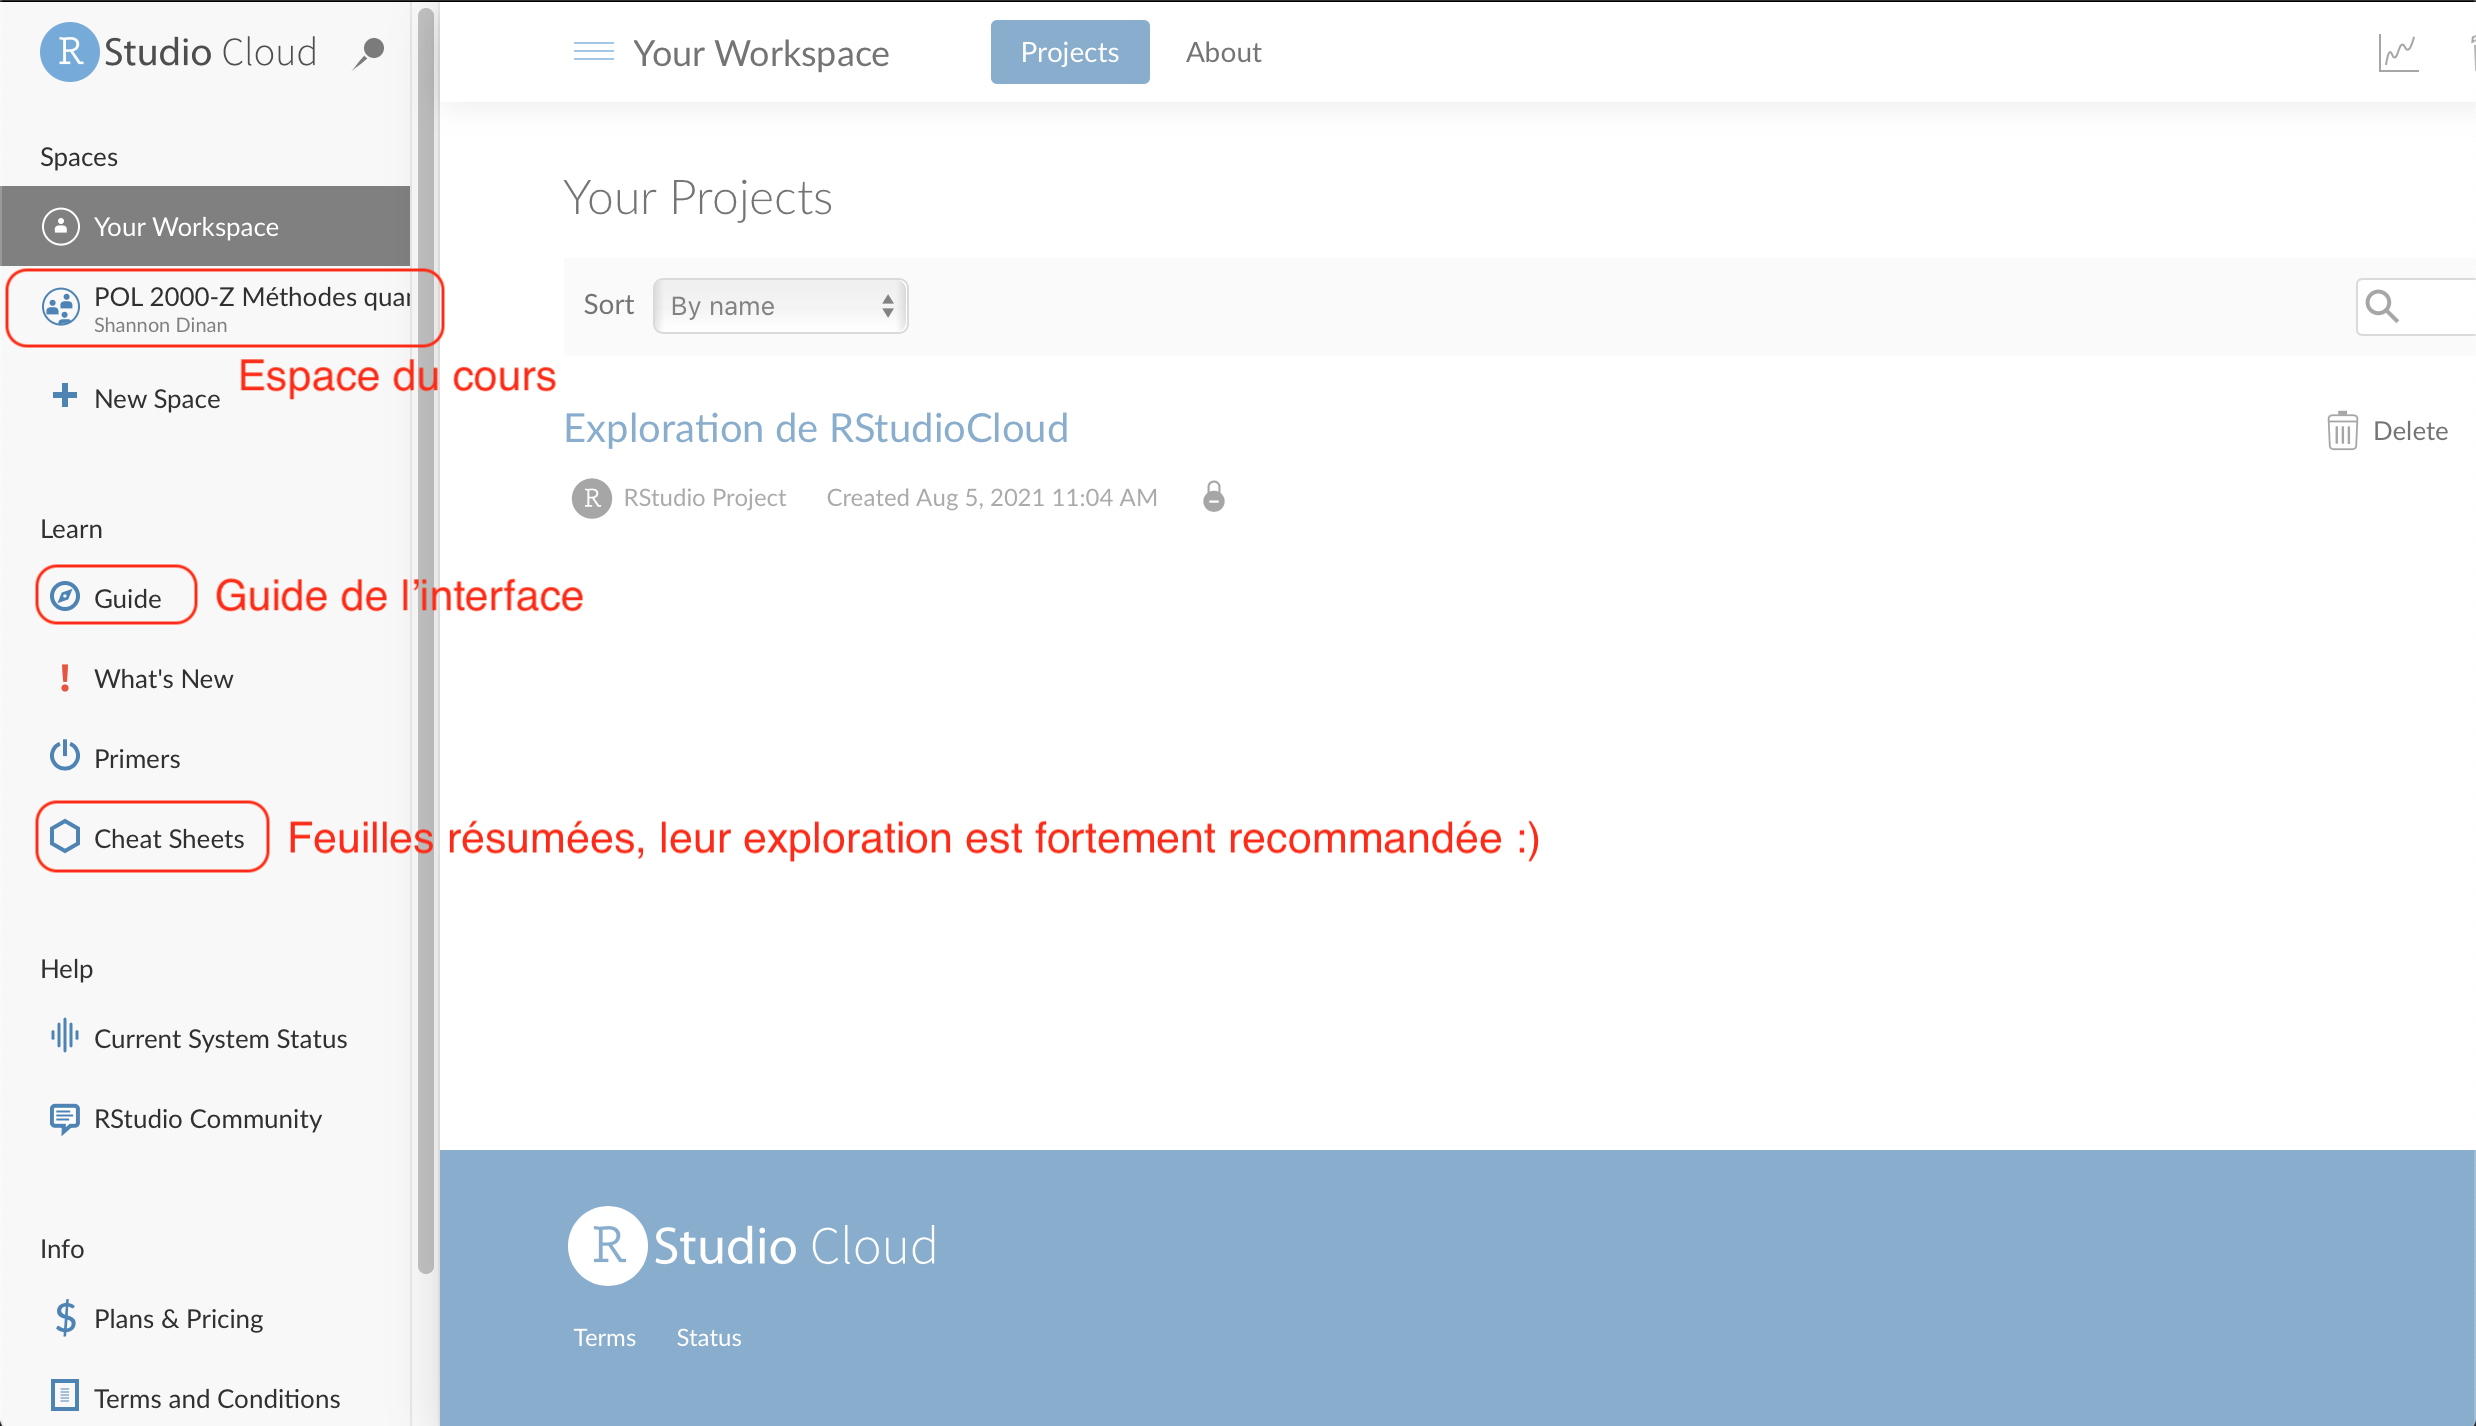
\includegraphics[width=1\linewidth]{_graphs/menupage.png}}
  \caption{Menu d'accueil}
  \label{homeMenu}
\end{figure}

\subsection{Interface}
  \textbf{RStudio Cloud} a deux interfaces, l'interface des espaces de travail et l'interface des projets. L'interface des espaces de travail est la première chose que vous rencontrez en vous connectant à \textbf{RStudio Cloud}. C'est ce qui vous permet de vous déplacer d'un projet à l'autre et d'un espace de travail à l'autre. La section \emph{menu} de cette interface offre aussi plusieurs liens menant à des ressources externes sur 1) l'utilisation de \textbf{RStudio Cloud}, 2) l'utilisation de \textbf{R} et 3) l'utilisation de ses \emph{packages} les plus populaires. Pour faciliter votre compréhension, les figures \ref{home} et \ref{homeMenu} présentent un aperçu de l'interface des espaces de travail de \textbf{RStudio Cloud} et ses principaux points d'intérêt.

La seconde interface est celle qui nous intéresse le plus, c'est l'endroit où vous écrirez et exécuterez votre code. La figure \ref{rstudio1} présente les points d'intérêt les plus importants. L'\emph{environnement} contiendra les bases de données que vous importerez ainsi que tous les objets créés lors de la session\footnote{Ici, \emph{session} fait référence à la période de travail sur \textbf{RStudio Cloud}.}. Nous aborderons les bases de données dans une section ultérieure. En dessous de l'\emph{environnement}, vous avez accès à vos dossiers, les librairies utilisées, un aperçu des graphiques produits ainsi qu'à de l'aide dans la fenêtre en bas à droite. La plus grande fenêtre par défaut est celle contenant la console. La \textbf{console} est un environnement d'exécution directe. En d'autres mots, vous pouvez y écrire des commandes qui seront exécutées immédiatement. C'est utile pour faire des tests et exécuter de petites manipulations. Or, la \textbf{console} n'enregistre pas la suite de commandes que vous lui demandez de faire, ce n'est pas son rôle. Pour ce faire, il faut ouvrir l'\textbf{éditeur} tel que spécifié par la figure \ref{rstudio1}. L'\textbf{éditeur}, c'est l'endroit où l'on écrit un code (une suite de commandes permettant d'atteindre un but quelconque, comme calculer une moyenne, faire une régression simple ou produire un graphique) afin qu'il puisse être enregistré et réutilisé. Dans le cadre de ce cours, vous allez principalement travailler dans l'\textbf{éditeur}.

Avant d'entrer dans la syntaxe d'utilisation de \textbf{R}, je recommande fortement la personnalisation de votre environnement. Non seulement cela vous permettra d'avoir une expérience esthétique plus agréable, cela vous aidera à long terme à reconnaître les structures du langage. Les figures \ref{rstudio2} et \ref{rstudio3} montrent comment accéder aux options de l'environnement global. Vous y trouverez ma mise en place préférée. Je tends à préférer coder sur fond plus foncé, mais je vous encourage à explorer les options et à trouver ce qui vous correspond le mieux. C'est pour vos yeux, pas ceux de l'équipe d'enseignement. 

\begin{figure}[H]
  \centering
  \fbox{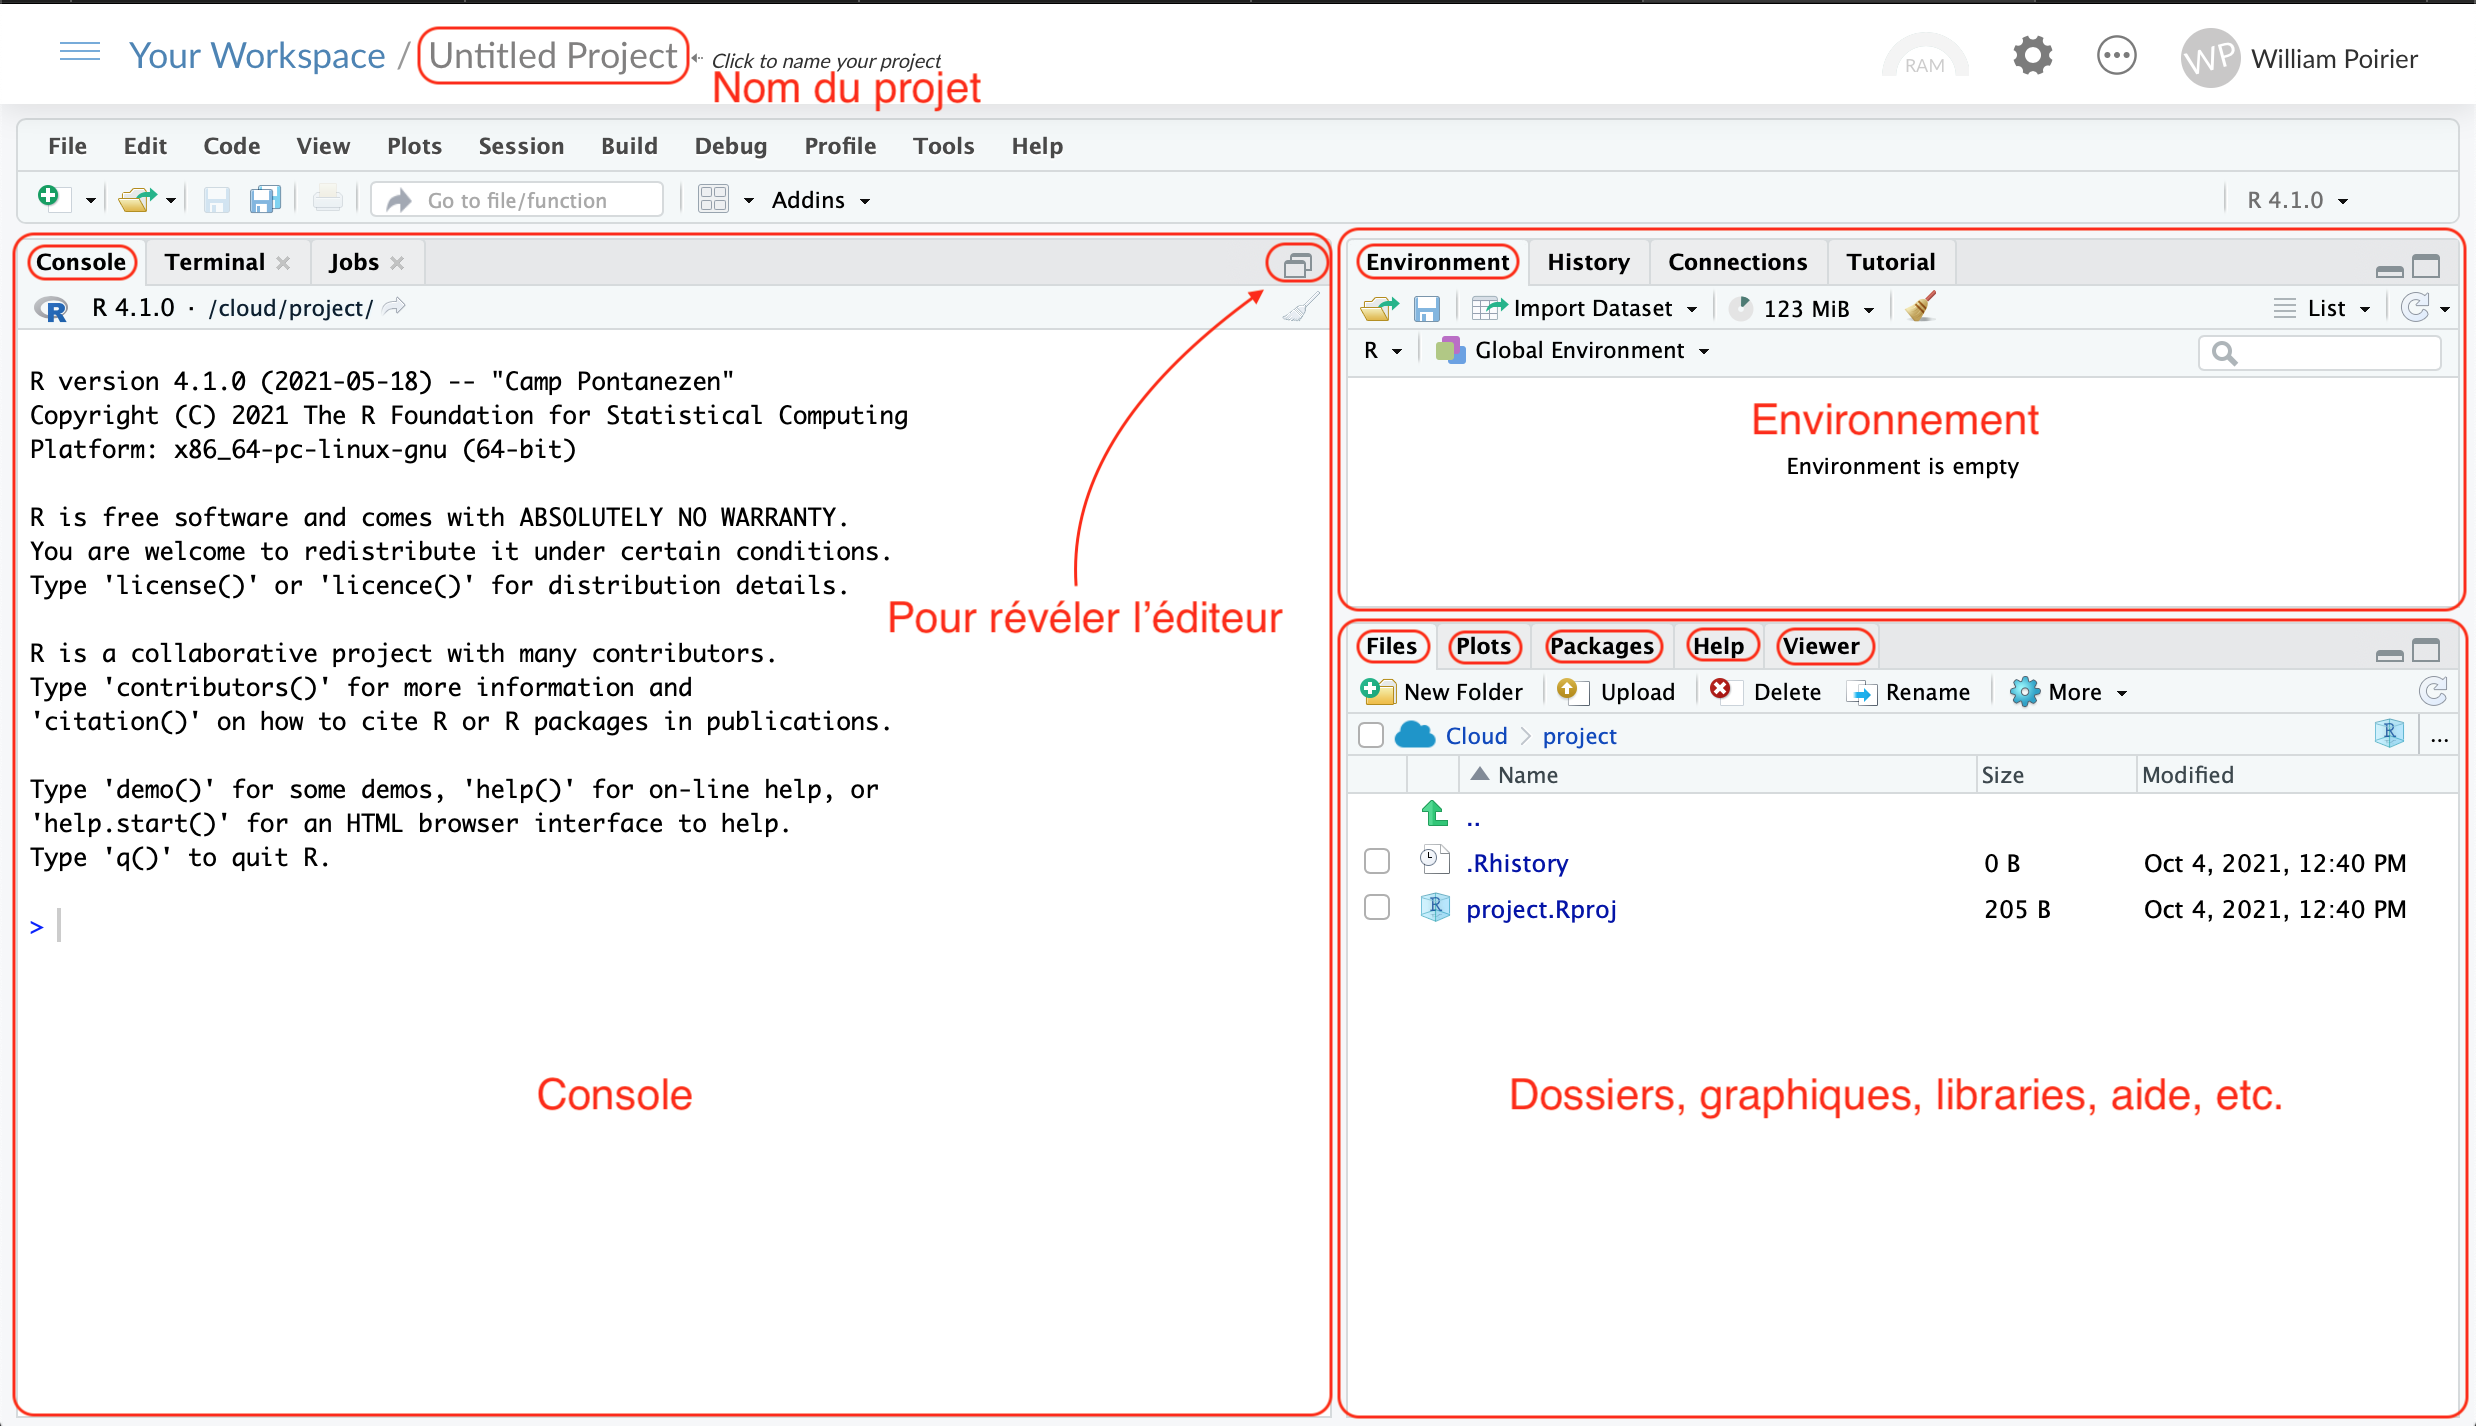
\includegraphics[width=0.98\linewidth]{_graphs/rstudio1.png}}
  \caption{État par défaut}
  \label{rstudio1}
\end{figure}

\begin{figure}[H]
  \centering
  \fbox{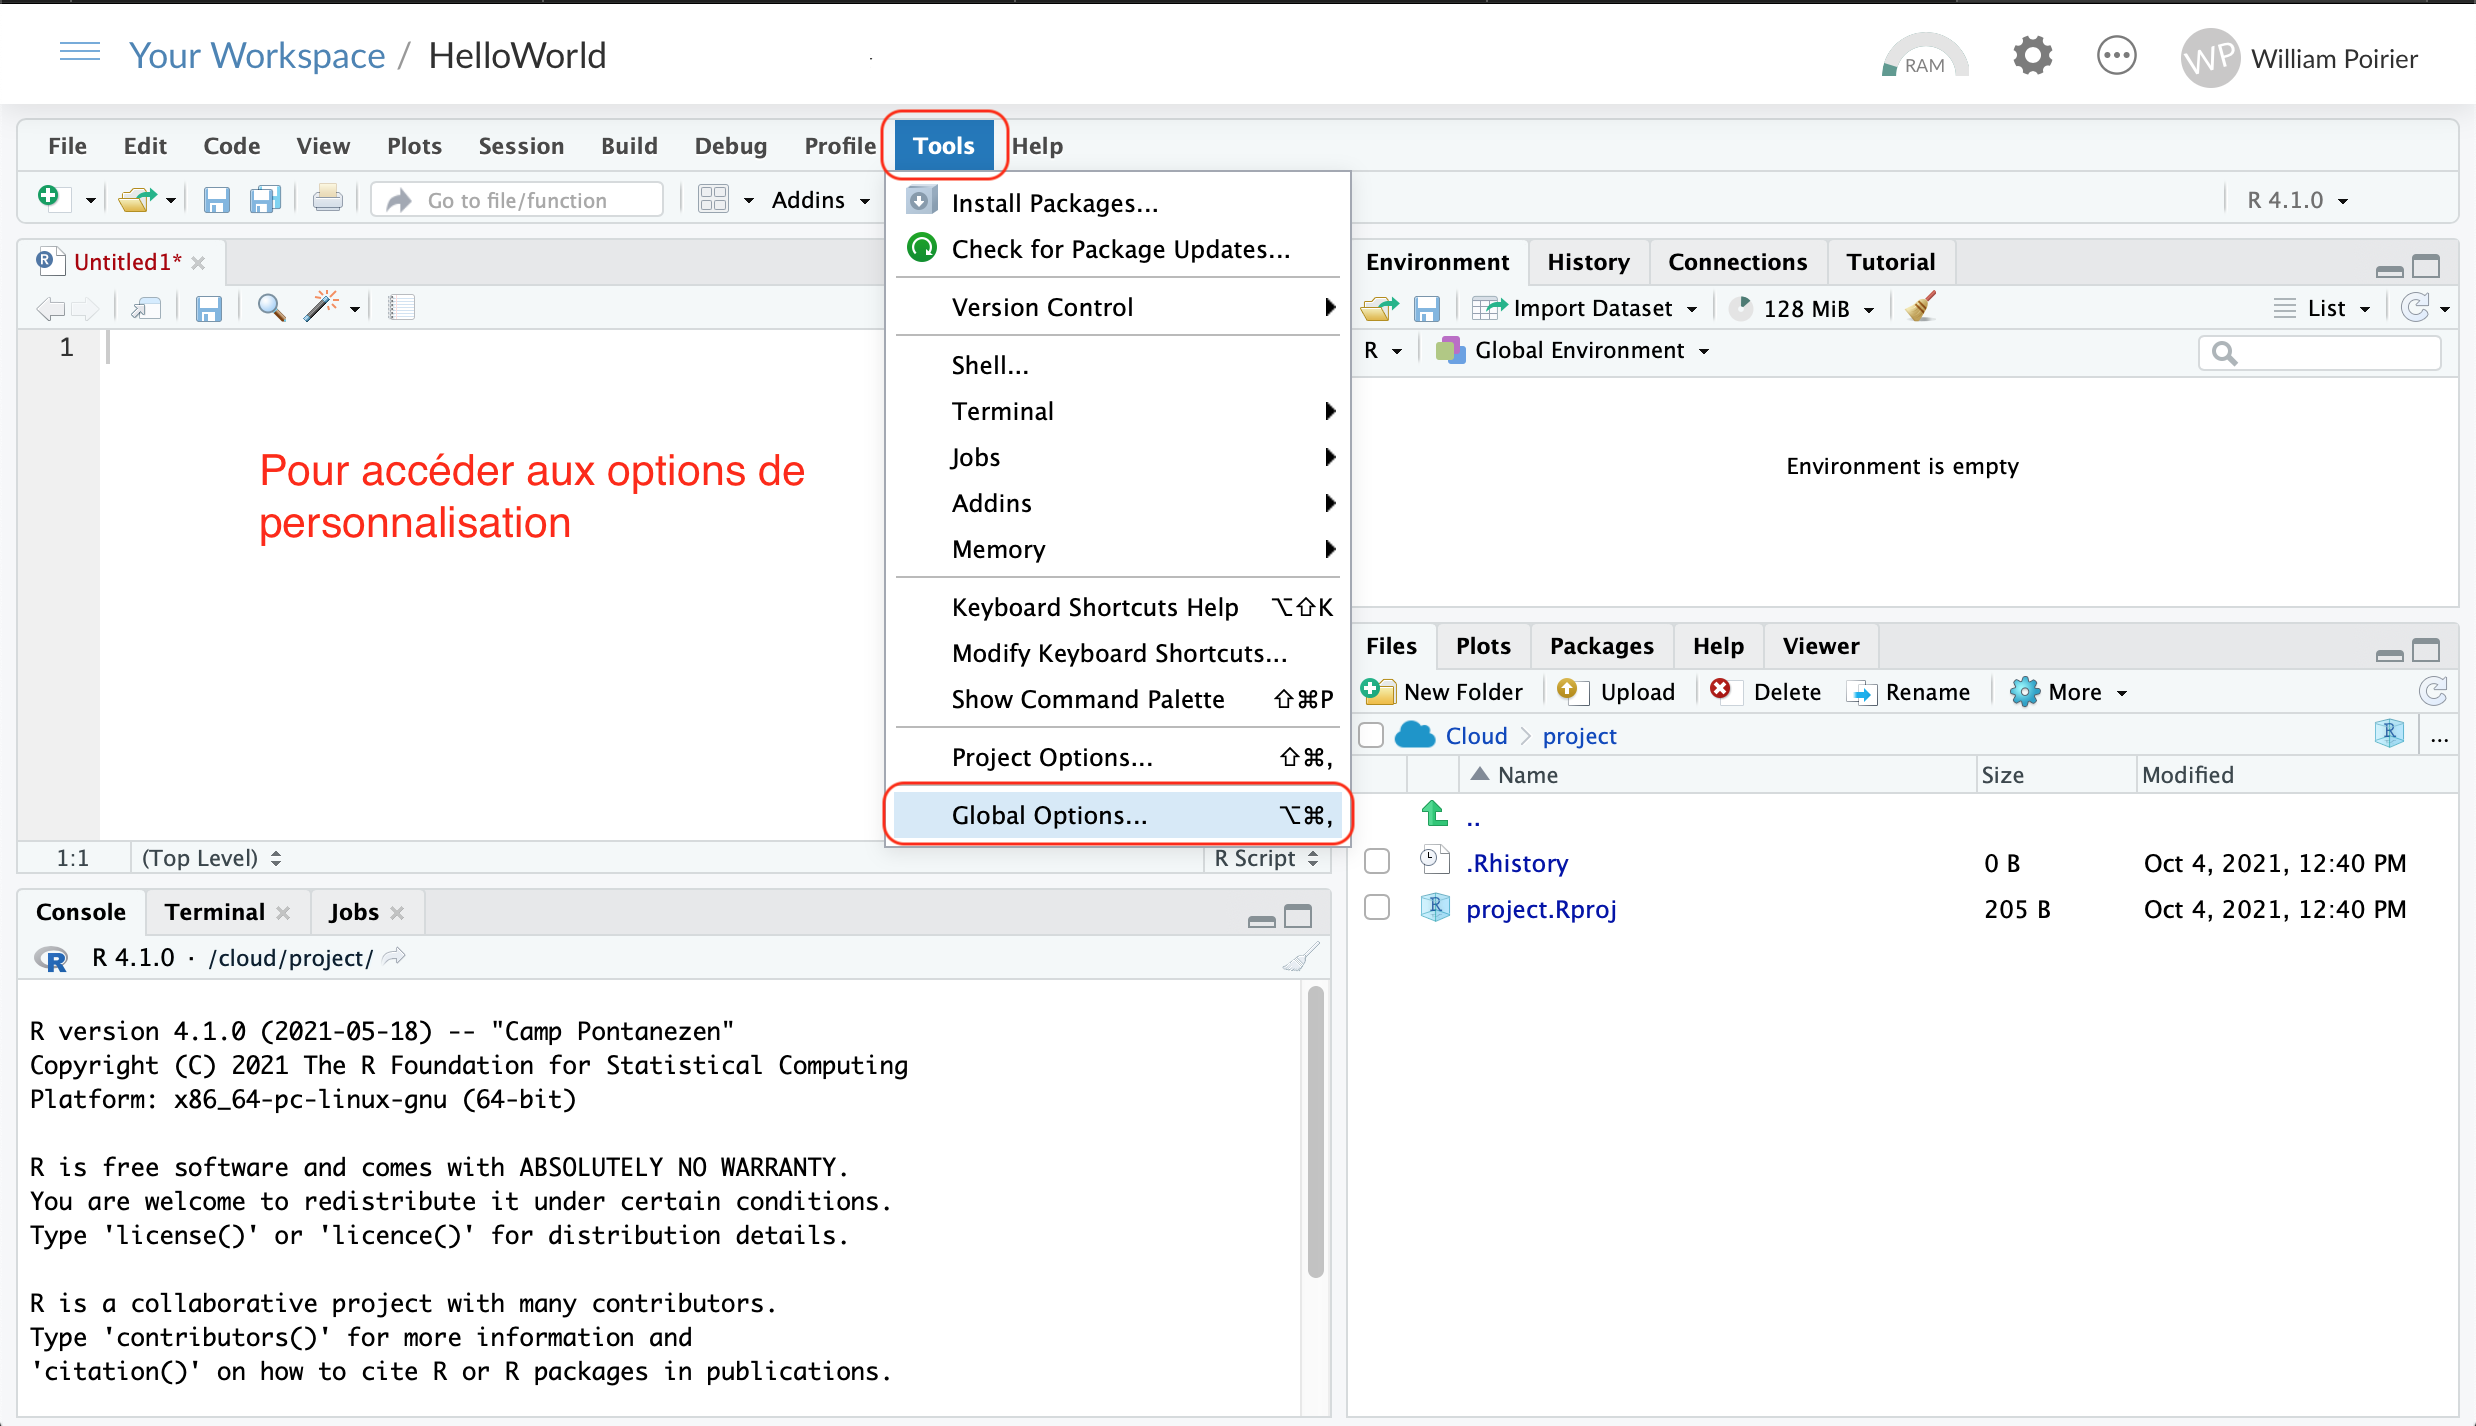
\includegraphics[width=0.98\linewidth]{_graphs/rstudio2.png}}
  \caption{Début de la personnalisation}
  \label{rstudio2}
\end{figure}

\begin{figure}[H]
  \centering
  \fbox{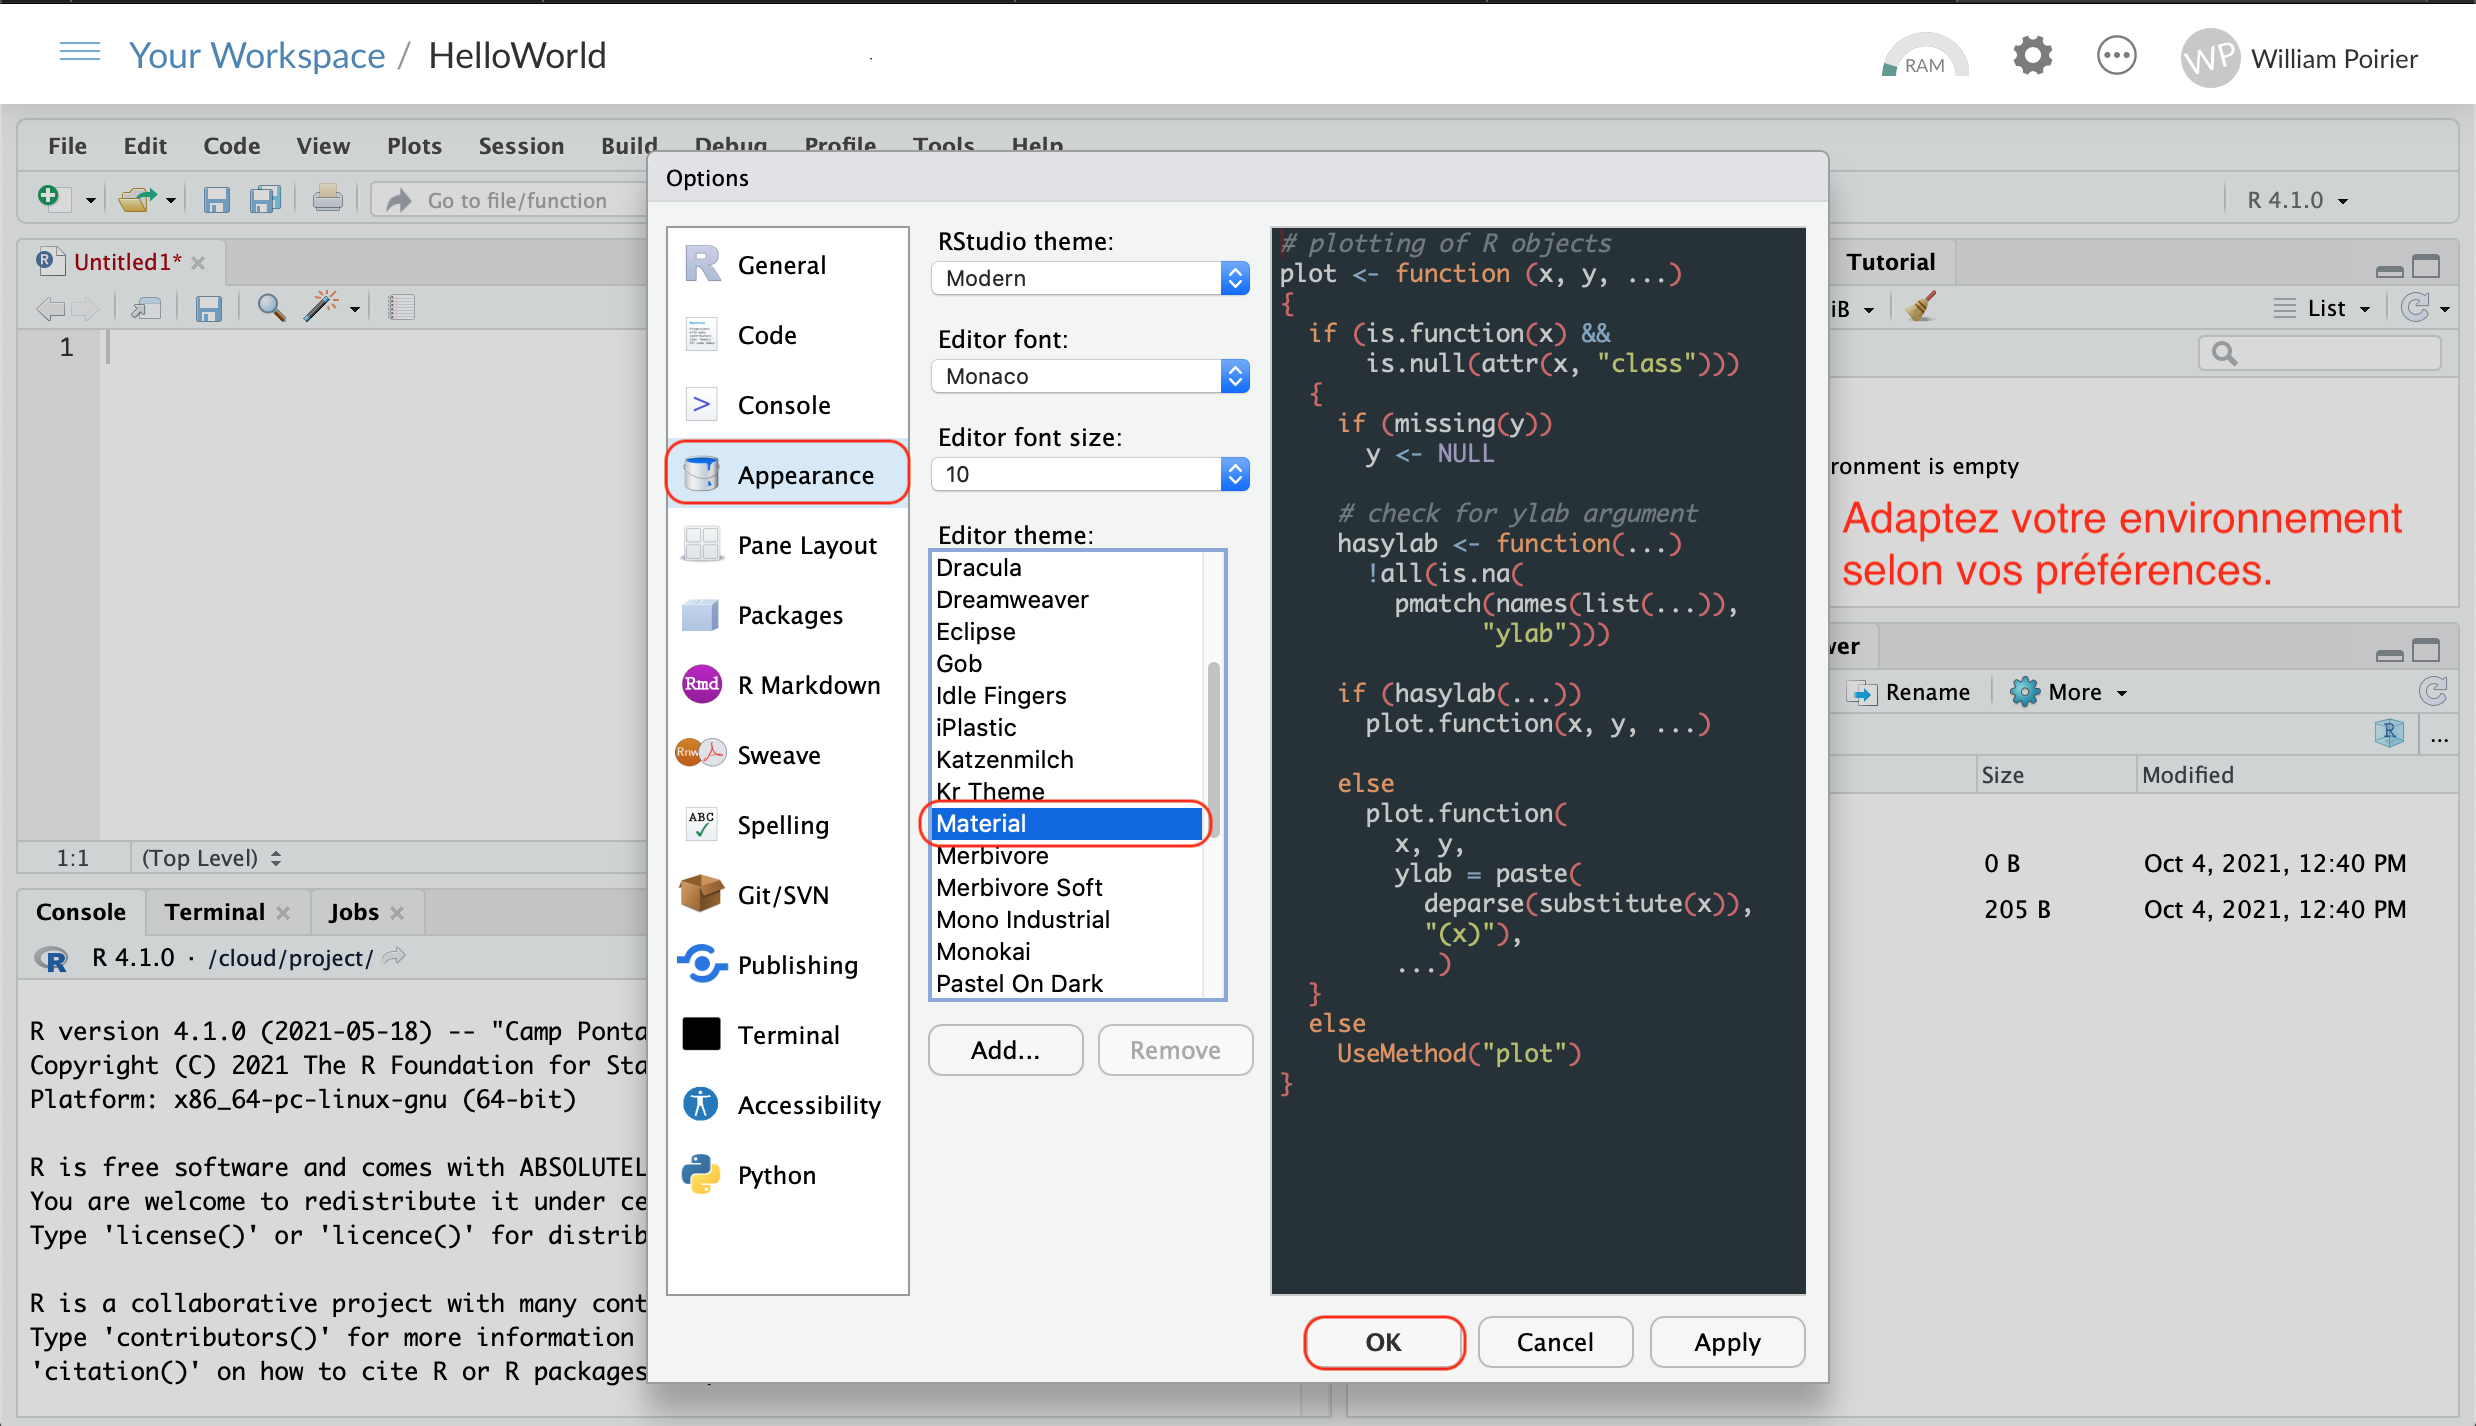
\includegraphics[width=0.98\linewidth]{_graphs/rstudio3.png}}
  \caption{Fin de la personnalisation}
  \label{rstudio3}
\end{figure}

\section{HelloWorld}

Vous en connaissez maintenant assez à propos de \textbf{R} pour rédiger votre première ligne de code! Allez dans l'éditeur, et tapez la commande suivante :
    \begin{lstlisting}
    > print("HelloWorld!")
    \end{lstlisting}
   
 Comme vous pouvez voir, \textbf{R} est un gentil programme qui fait une partie du travail pour vous. Dès que vous ouvrez une parenthèse dans l'éditeur, le logiciel ajoute déjà la seconde parenthèse pour s'assurer qu'il n'y ait pas de message d'erreur. \textbf{R} fait la même chose pour les guillemets. 
   
À présent, il faut exécuter votre ligne de code. Pour ce faire, sélectionnez la ligne, puis cliquez sur le bouton \textit{\textbf{RUN}} en haut à droite. La figure \ref{rstudio4} vous montre un exemple. Une fois exécuté, ce simple code imprimera n'importe quelle suite de caractères que vous aurez choisi. Amusez-vous!

Remarquez que le résultat s'affiche dans la console en bas. C'est sa deuxième utilité. La console vous indique les résultats des commandes que vous exécutez à partir de l'éditeur. Félicitations, vous êtes désormais des programmeurs, le fun peut commencer! 

ATTENTION! Pour la suite du tutoriel, je vous invite tout de suite à repérer ces symboles sur votre clavier d'ordinateur : \rcode{<}, \rcode{>}, \rcode{=}, \rcode{"}, \rcode{'}, \rcode{\$}, \rcode{|}, \rcode{\&}, \rcode{\%}, \rcode{[}, \rcode{]}, \rcode{\{}, \rcode{\}}.

\begin{figure}[H]
  \centering
  \fbox{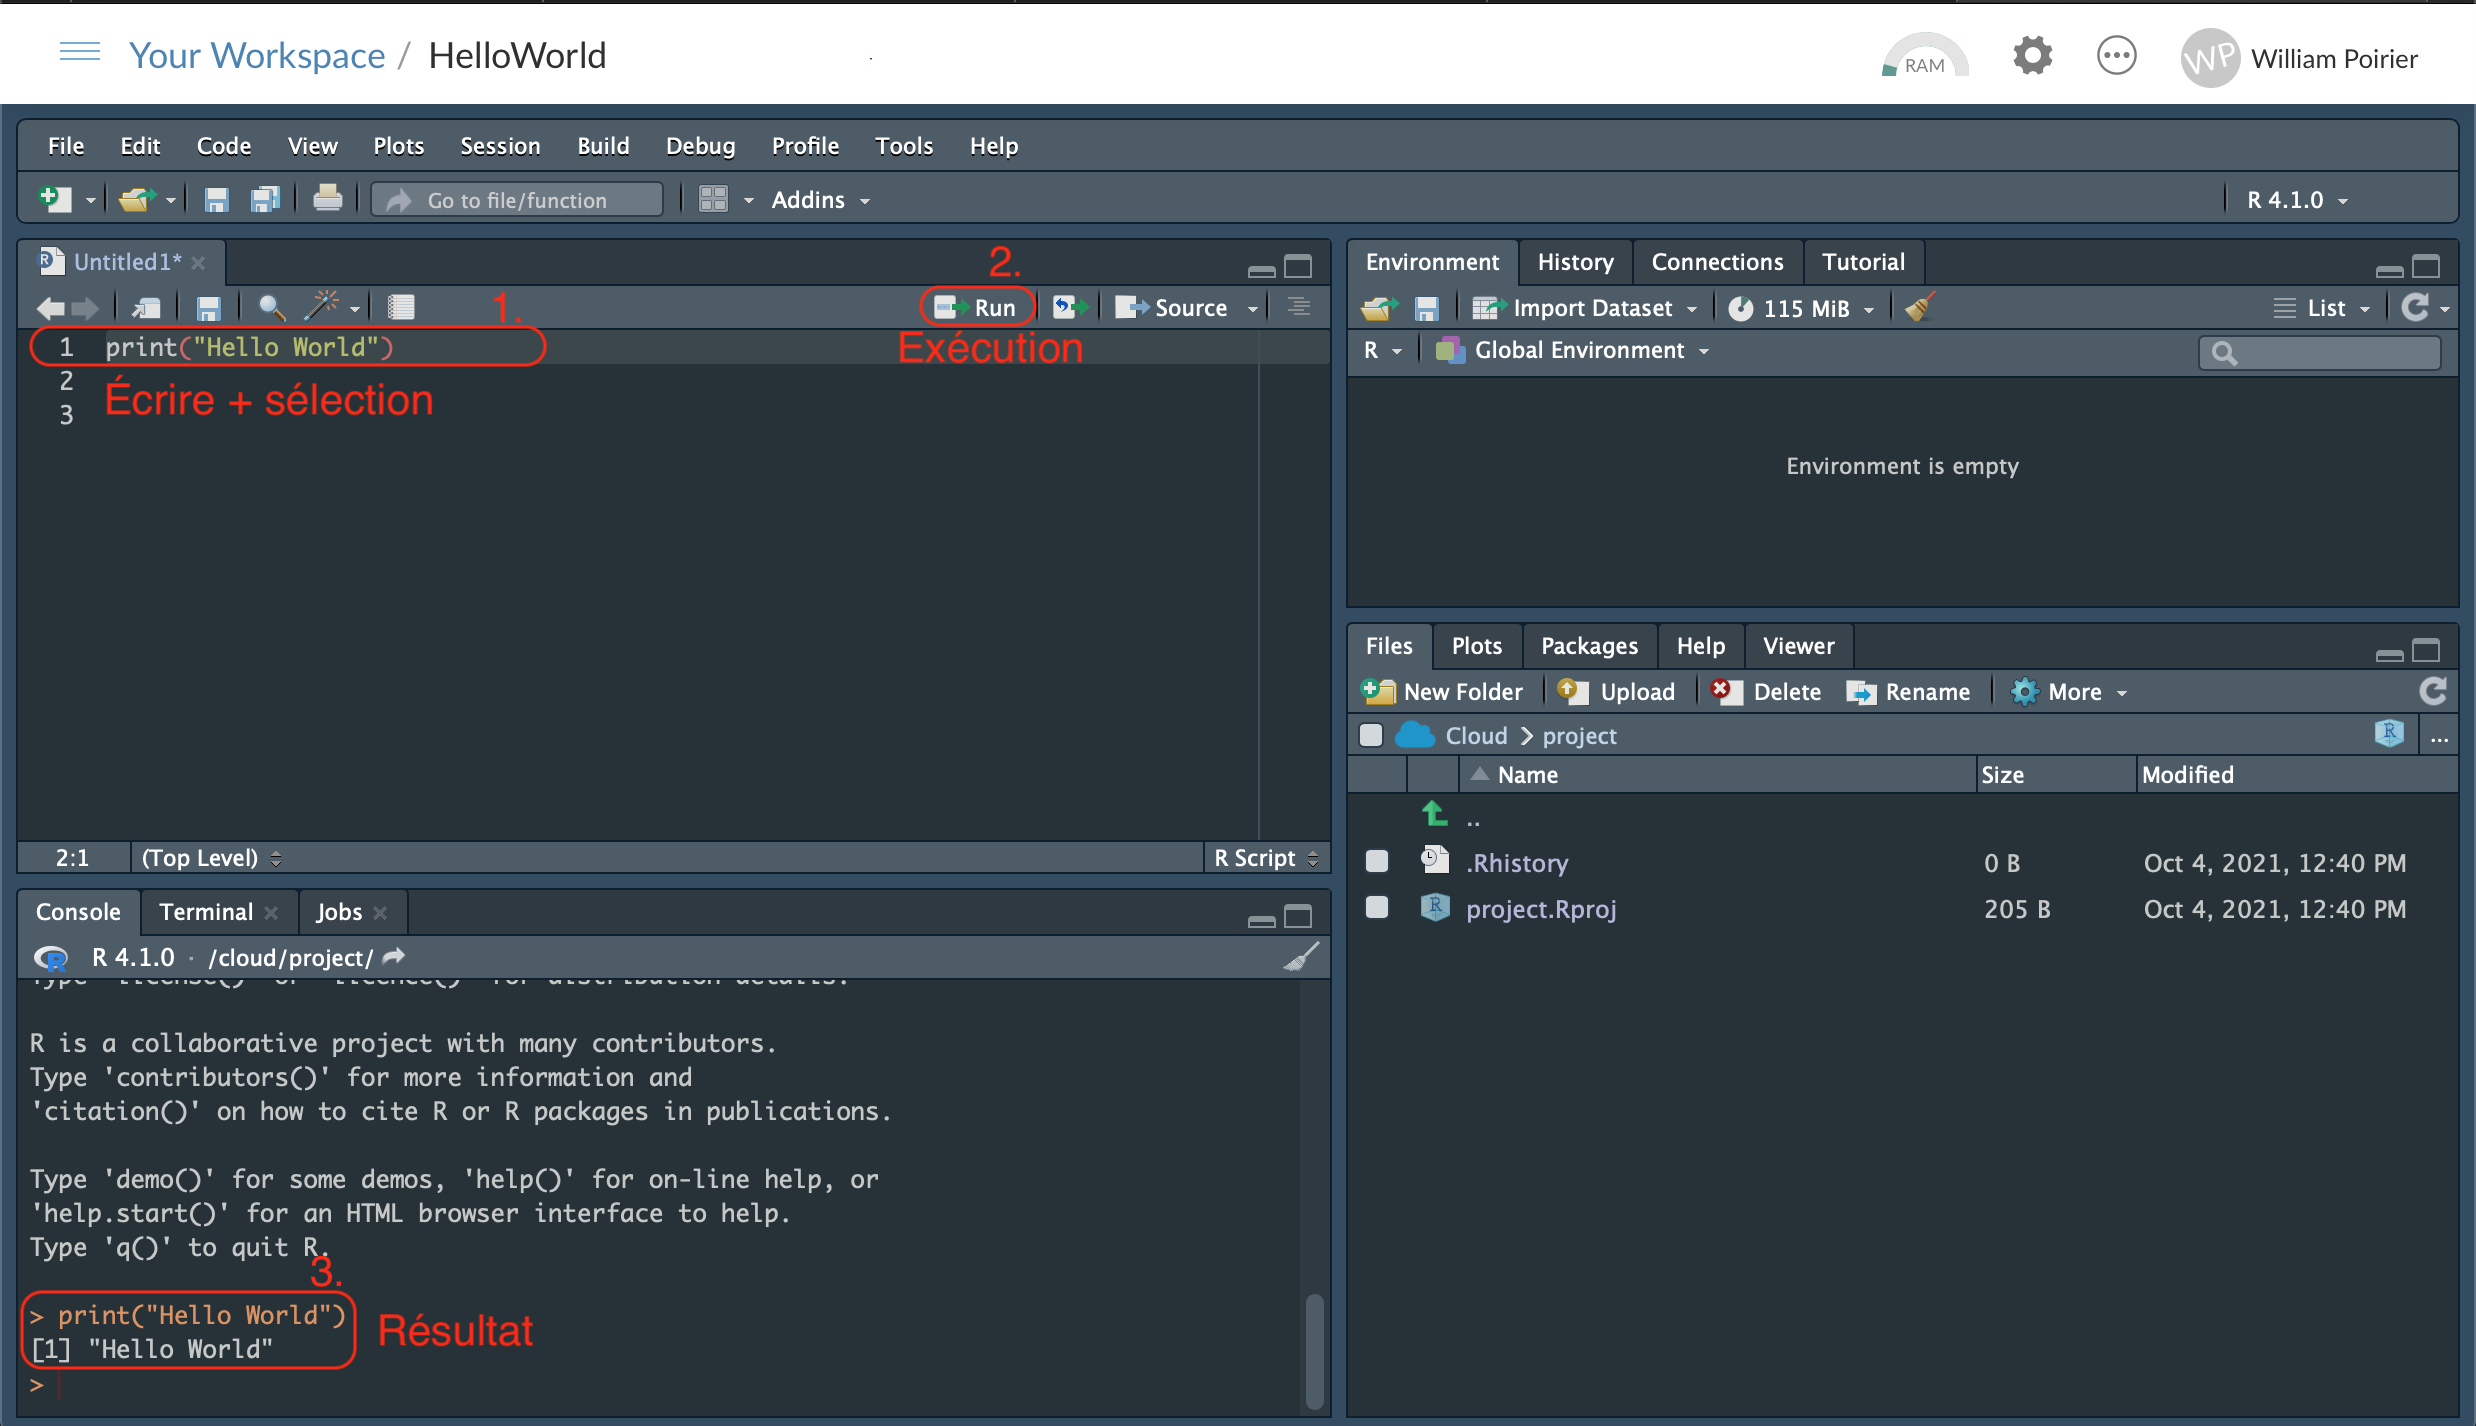
\includegraphics[width=0.98\linewidth]{_graphs/rstudio4.png}}
  \caption{Votre première ligne de code!}
  \label{rstudio4}
\end{figure}

  \subsection{Workflow}
  
  Un facteur important à prendre en considération lorsque l'on programme ou que l'on gère des bases de données, c'est l'organisation de notre « \emph{flux de travail} ». Plusieurs éléments sont à considérer lorsque l'on veut optimiser son travail. Nous aborderons les principaux dans cette section. Ces habitudes peuvent vous aider à éviter des situations fâcheuses.
  
    \subsubsection{Arborescence}
    Si vous lisez le titre de cette section sans savoir ce à quoi nous faisons référence, ne vous inquiétiez pas. La plupart des gens utilisent l'arborescence de leur ordinateur sans même s'en rendre compte. C'est tout simplement le chemin par lequel vous (ou votre ordinateur) devez passer pour accéder à un fichier. Comme quand vous voulez retrouver un vieux travail, votre ordinateur doit savoir où se trouvent les fichiers que vous mobilisez dans votre code. Pour ce faire, il faut établir le « répertoire de travail » (\emph{working directory}) de la session \textbf{R}. On utilise alors la fonction \rcode{setwd()} et on y inscrit l'arborescence (le chemin) :
    
    \begin{lstlisting}
    # Pour les Mac
    > setwd("/Users/nomDelaSession/nomDuDossier/nomDuSousDossier")
    # Pour les PC
    > setwd("C:/Users/nomDelaSession/nomDuSousDossier")
    \end{lstlisting}
    
    Remarquez la façon dont l'arborescence est écrite. Chaque dossier est suivi d'une barre oblique (/) et d'un sous-dossier. C'est donc important de bien organiser les dossiers sur son ordinateur de sorte à éviter de devoir changer de répertoire de travail trop souvent. L'idéal c'est de référer à un dossier général contenant les dossiers spécifiques. Par exemple, si vous travaillez sur un projet de recherche à propos des élections fédérales en 2021, vous pourriez avoir un dossier \rcode{ElectionFed21} qui contient un dossier \rcode{codeR}, un dossier \rcode{graphs} et un dossier \rcode{Data}. De cette façon, vous pouvez indiquer un répertoire de travail général au début de votre code pour ensuite utiliser des arborescences relatives. Ne vous inquiétez pas, tout ceci deviendra très simple au cours de la session.
    
    \subsubsection{Commentaires}
    
    Commenter un code c'est l'habitude la plus importante à prendre, surtout lorsqu'on est en apprentissage. Que voulons-nous dire par là? Imaginez que vous êtes en train d'explorer une forêt. Vous pourrez sans doute retrouver votre chemin de mémoire, mais l'idéal c'est de laisser des repères tout au long du chemin. Surtout si vous n'y retournerez pas avant un moment. Coder, c'est la même chose. Vous allez développer une suite d'instructions logiques qui permettra de produire un résultat spécifique. Il faut donc vous assurer de pouvoir bien comprendre les différentes étapes de votre code, et ce, même après plusieurs mois ou années. La mémoire étant une faculté qui oublie, ce n'est peut-être pas l'outil le plus fiable pour cette tâche. Donc, pour commenter, il vous suffit de précéder ce que vous écrivez par un \rcode{$\#$}. Voici un exemple dans lequel nous avons divisé les réponses à une variable (qui variait entre 0 et 1) en trois catégories distinctes :
    
    \begin{lstlisting}
    # Separation en trois niveaux de la variable ses_health
    > Data$ses_health[Data$ses_health==0.75 | Data$ses_health==1] <- 1 
    > Data$ses_health[Data$ses_health==0.5] <- 0.5
    > Data$ses_health[Data$ses_health==0.25 | Data$ses_health==0] <- 0
    \end{lstlisting}
    
    \subsubsection{Raccourcis clavier}
    
   Écrire des lignes de code peut être frustrant, surtout lorsque vous n'êtes pas habitué à repérer certains symboles comme [ ] et \{ \}. Comme dans toute chose, avec de l'expérience, vous allez acquérir de la rapidité. Par ailleurs, certains raccourcis clavier de \textbf{RStudio} et \textbf{RStudio Cloud} pourront vous éviter de perdre de précieuses secondes. Puisque ces raccourcis vont varier en fonction du système d'opération de votre ordinateur, les deux prochaines sections s'adressent aux utilisateurs Mac et PC respectivement. 
    
      \paragraph{Raccourcis clavier -- Utilisateurs Mac}
      \begin{enumerate}
        \item \rcode{cmd + enter}, permet de rouler la partie du code sélectionné.
        \item \rcode{option + sélection}, permet de sélectionner une portion de plusieurs lignes en même temps. Voir la figure~\ref{altSelect}.
        \item \rcode{shift + flèches}, permet de sélectionner à l'aide des flèches (gauche, droite, bas, haut) du clavier.
        \item \rcode{cmd + flèches}, permet d'accéder au début (avec la flèche du haut) et à la fin (avec la flèche du bas) d'un document.
        \item \rcode{option + flèche}, permet d'inverser une ligne avec celle du haut (avec la flèche du haut) ou avec celle du bas (avec la flèche du bas).
      \end{enumerate}
      
      \paragraph{Raccourcis clavier -- Utilisateurs PC}
      \begin{enumerate}
        \item \rcode{ctrl + enter}, permet de rouler la partie du code sélectionné.
        \item \rcode{alt + sélection}, permet de sélectionner une portion de plusieurs lignes en même temps. Voir la figure \ref{altSelect}.
        \item \rcode{shift + flèches}, permet de sélectionner à l'aide des flèches (gauche, droite, bas, haut) du clavier.
        \item \rcode{ctrl + flèches}, permet d'accéder au début (avec la flèche du haut) et à la fin (avec la flèche du bas) d'un élément du code.
        \item \rcode{alt + flèche}, permet d'inverser une ligne avec celle du haut (avec la flèche du haut) ou avec celle du bas (avec la flèche du bas).
      \end{enumerate}
      
            \begin{figure}[H]
      \centering
      \fbox{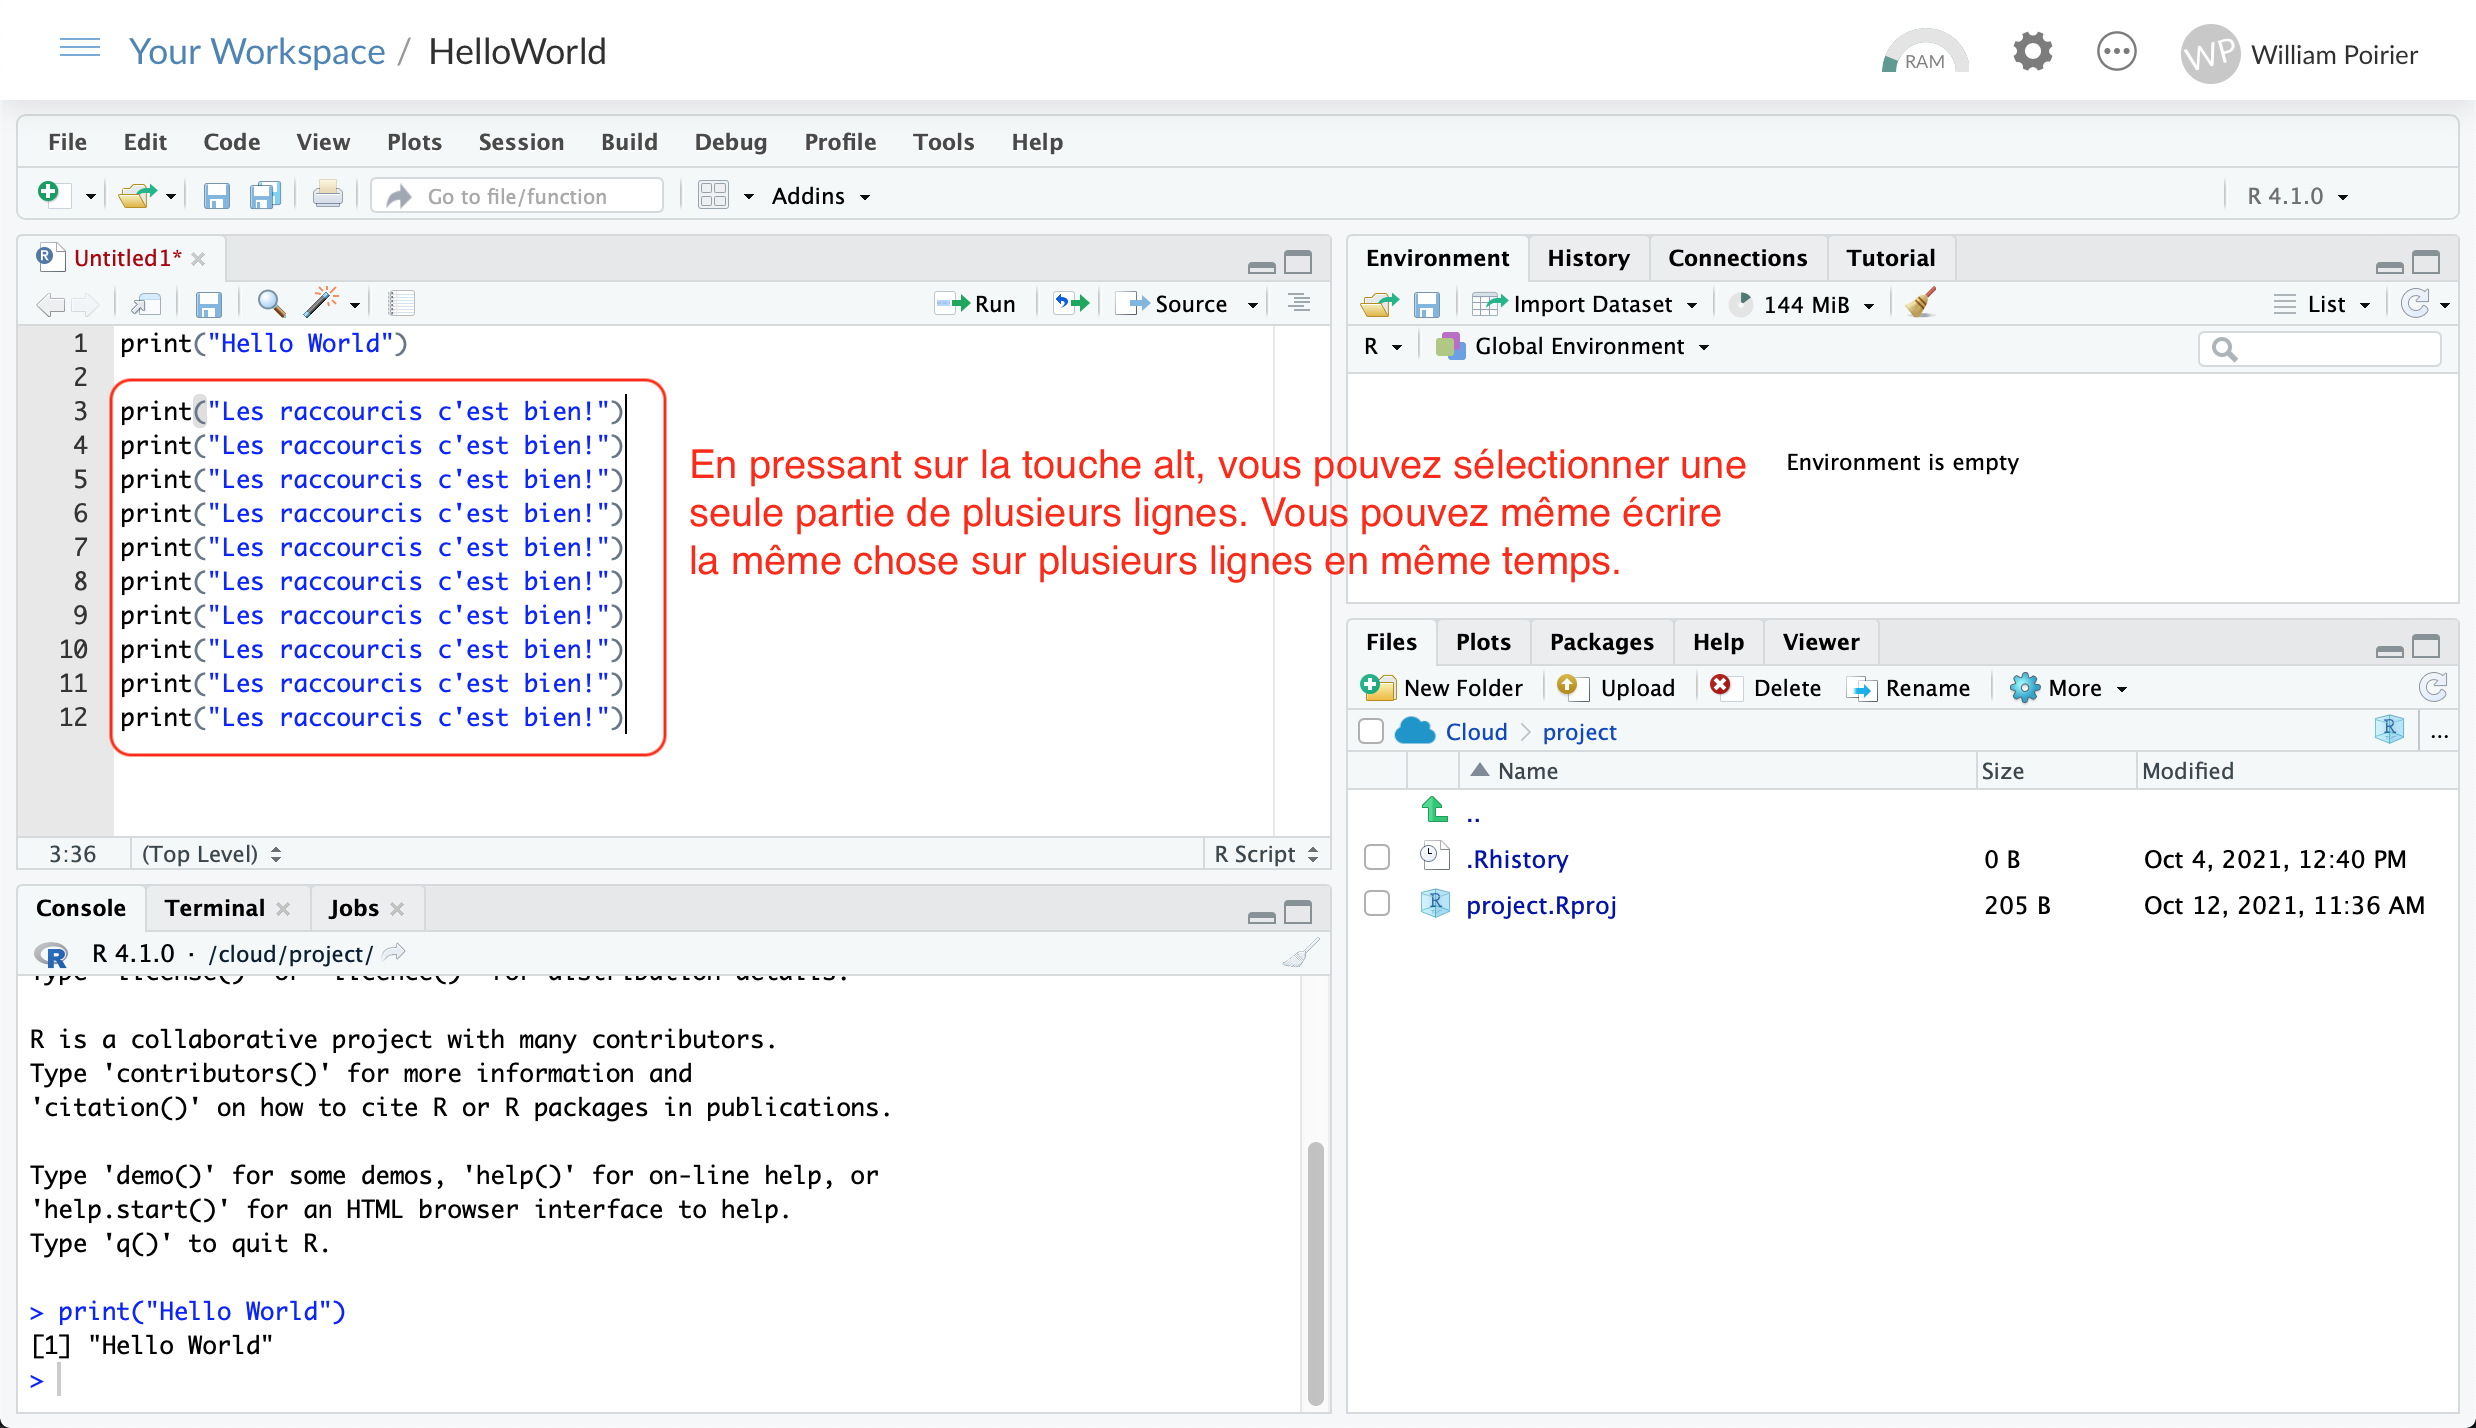
\includegraphics[width=0.98\linewidth]{_graphs/altSelect.png}}
      \caption{Sélection multiple de lignes}
      \label{altSelect}
      \end{figure}
      
\section{Intro à la programmation en R}
Vous connaissez le logiciel \textbf{R} et vous avez de bonnes habitudes de codage. Nous pouvons désormais entrer dans le vif du sujet, la programmation en \textbf{R}. Que vous utilisiez \textbf{RStudio} ou \textbf{RStudio Cloud}, les prochaines indications ne changent pas. 
      
  \subsection{Ça va bien aller}
  Plusieurs étudiants sont anxieux face à la tâche d'apprendre un langage de programmation. C'est tout à fait normal. La programmation vient avec une aura cryptique, un jargon et des programmeurs qui ne sont pas toujours à même d'expliquer ce qu'ils font. Or, pour ce cours, nous considérerons \textbf{R} comme une calculatrice +, c'est-à-dire comme un outil permettant d'effectuer des opérations mathématiques plus ou moins complexes. Vous ne deviendrez pas des développeurs à la fin de ce cours et ce n'est pas l'objectif. Le but est plutôt de vous former pour que vous soyez en mesure d'effectuer des analyses de base, une compétence qui vous distinguera sur le marché du travail.

Ceci étant dit, vous allez avoir besoin d'aide à un moment, c'est certain. L'équipe d'enseignement est, bien entendu, disponible pour répondre à vos questions. Cependant, nous préférons que vous développiez votre autonomie. Pour ce faire, nous vous encourageons à consulter les ressources en ligne mentionnée à la section \ref{R vs RStudio vs RStudio Cloud}. D'autres ressources sont également offertes par \textbf{R} lui-même. En précédant toute fonction d'un \rcode{?} dans la console \footnote{Lorsqu'une fonction n'est pas dans votre environnement de travail et que vous utilisez \rcode{?ggplot()}, \textbf{R} retournera une erreur du genre « \textcolor{BlueViolet}{\rcode{Error in .helpForCall(topicExpr, parent.frame()) : no methods for ‘ggplot’ and no documentation for it as a function}} ». Lorsque c'est le cas, vous pouvez précéder la fonction d'un double \rcode{?}. Ceci indiquera à \textbf{R} de chercher dans toute la documentation des serveurs de CRAN.}:

  \begin{lstlisting}
    # Dans la console, pour obtenir de l'aide pour la fonction sample()
    > ?sample()
  \end{lstlisting}
  
  \subsection{Opérateurs}
 Comme vous avez certainement déjà saisi, au lieu d'avoir une interface qui vous permet de cliquer sur les boutons et onglets, la plupart des actions en \textbf{R} se font à l'aide d'\emph{opérateurs}. Ceux-ci sont simplement des symboles utilisés pour diriger le programme à faire des actions quelconques. C'est donc en manipulant ces opérateurs qu'il soit possible de calculer une moyenne, de faire un graphique, ou même de faire de l'apprentissage machine. Ainsi, les différents types d'opérateurs sont la base de la programmation en \textbf{R}. Nous pouvons sous-diviser les opérateurs et différents types. Les prochaines sections vous présenteront aux opérateurs de bases auxquels vous allez avoir affaire dans le cadre du cours. 
 
 \begin{figure}[H]
    \centering
    \fbox{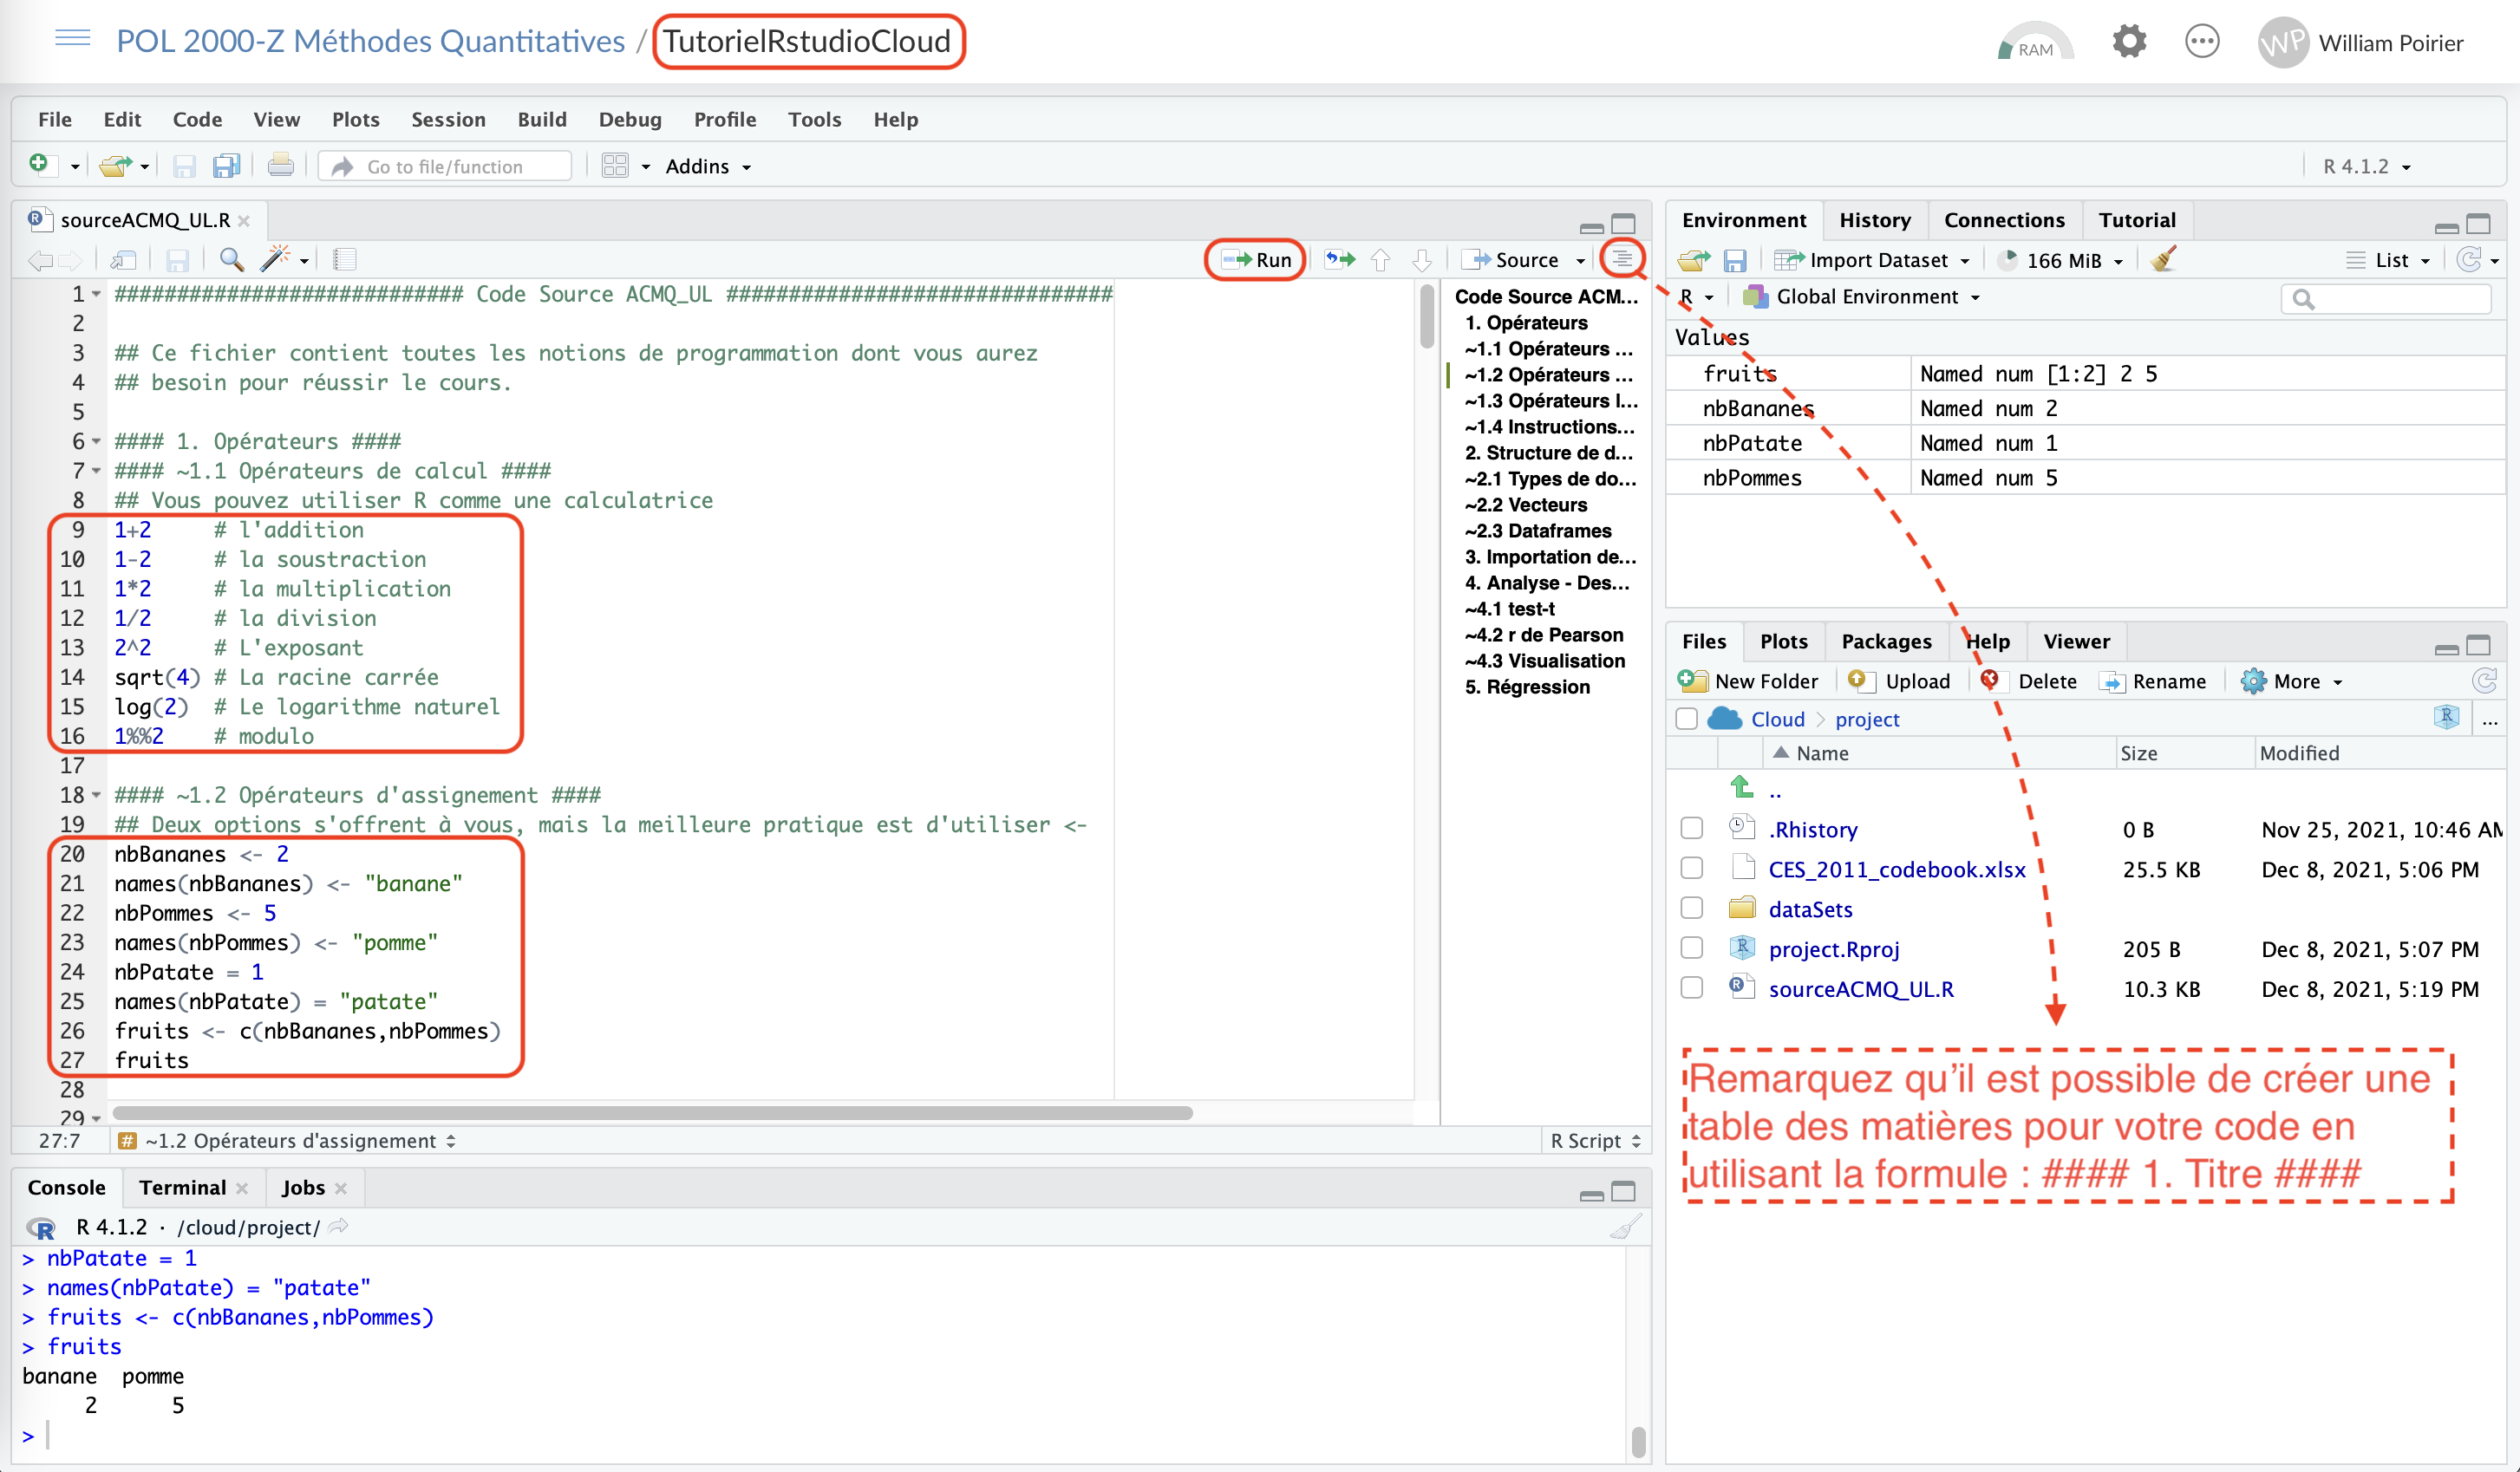
\includegraphics[width=0.98\linewidth]{_graphs/opeAssign.png}}
    \caption{Opérateurs de calcul et d'assignement}
    \label{opeAssign}
    \end{figure}
  
    \subsubsection{Opérateurs de calcul}
    Les opérateurs de calcul sont les opérateurs mathématiques que vous connaissez (\rcode{+},\rcode{-},\rcode{*},\rcode{/}).\footnote{Il existe aussi l'opérateur modulo (\rcode{\%\%}) qui permet de calculer le reste d'une division euclidienne. C'est pratique pour identifier si un nombre est un diviseur d'un autre nombre.} Ces opérateurs sont aussi visibles dans l'éditeur à la figure \ref{opeAssign}. Tout comme une calculatrice, vous pouvez utiliser ces opérateurs pour faire des calculs. Essayez :
    
  \begin{lstlisting}
    # Calcul pour obtenir la moyenne de cet échantillon fictif de 5 cas : 8, 12, 15, 19, 20
    > (8 + 12 + 15 + 19 + 20) / 5
  \end{lstlisting}

Mais cette façon de procéder est peu productive. Nous verrons les commandes pour les mesures de la centralité et de dispersion à la section \ref{vec}.

    \subsubsection{Opérateurs d'assignement}
    Les opérateurs d'assignement, comme leur nom l'indique, permettent d'assigner des valeurs à des objets. Voici un exemple avec la moyenne que nous venons de calculer. Une fois exécuté, la console retournera la réponse « 14.8 » lorsque nous écrivons la moyenne dans l'éditeur et que l'on clique sur « Run ». Vous pouvez voir d'autres exemples de l'éditeur dans la figure \ref{opeAssign}.
    
  \begin{lstlisting}
    # Assigner le calcul précédent à l'objet "moyenne"
    > moyenne <- (8 + 12 + 15 + 19 + 20) / 5
  \end{lstlisting}

Lorsque vous utilisez des opérateurs d'assignement, deux options s'offrent à vous. Vous pouvez utiliser le signe d'égalité (\rcode{=}) ou utiliser la flèche d'assignement (\rcode{<-}). Même si utiliser le signe d'égalité est plus intuitif pour la plupart d'entre vous, il est fortement recommandé d'utiliser la flèche d'assignement (\rcode{<-}). Pourquoi? Il s'agit d'un standard de bonne pratique. Souvent en programmation, il y a plusieurs façons d'arriver au même résultat. Les standards de bonne pratique nous permettent d'identifier les pratiques optimales sans avoir à comprendre pourquoi une pratique est meilleure qu'une autre dans toutes ses nuances. Pour ce cours, utilisez la flèche d'assignement (\rcode{<-}). 
    
    \subsubsection{Opérateurs logiques}
    Les opérateurs logiques retournent l'une de deux valeurs, soit « vrai » ou « faux ». Ils sont donc utilisés pour comparer deux objets. Voici les principaux : 
    \begin{itemize}
      \item A \rcode{<} B    : A est plus petit que B
      \item A \rcode{>} B    : A est plus grand que B
      \item A \rcode{<=} B   : A est plus petit ou égal à B
      \item A \rcode{>=} B   : A est plus grand ou égal à B
      \item A \rcode{==} B   : A est égal à B
      \item A \rcode{!=} B   : A n'est pas égal à B
      \item \rcode{\&}       : Une condition \textbf{ET} une autre condition
      \item \rcode{|}        : Une condition \textbf{OU} une autre condition
      \item A\rcode{\%in\%}B : A est contenu dans B
    \end{itemize}
    
    La figure \ref{opeLogi} contient une série de tests logique (lignes 29 à 38) qui peuvent servir d'exemple. Cependant, nous vous suggèrons fortement de tenter d'y répondre dans votre tête avant d'exécuter chaque ligne. 
   
       \begin{itemize}
      \item \rcode{if} (\emph{condition}) \{\emph{suite d'opération}\}
      \item \rcode{else} \{\emph{suite d'opération}\}
      \item \rcode{for} (\emph{facteur d'itération}) \{\emph{suite d'opération}\}
    \end{itemize}
     
    \subsubsection{Instructions de contrôle}
  Jusqu'à présent, \textbf{R} ne se distingue pas beaucoup d'une calculatrice. Les instructions de contrôle sont ce qui rend \textbf{R} beaucoup plus puissant que votre calculatrice. En effet, elles permettent d'automatiser des procédures et des calculs. Trois instructions de contrôle principales sont à retenir :
    
    Les instructions de contrôle sont souvent ce qu'il y a de plus difficile à apprendre lorsqu'on commence à programmer. \emph{Leur maîtrise n'est donc pas essentielle pour la réussite de ce cours}. Il est cependant important que vous ayez connaissance de leur existence. Vous avez un exemple à la figure \ref{opeLogi}. %Je vous donne donc le défi de bien comprendre ce qui se passe dans le script de l'exemple à la figure \ref{opeLogi}. Vous remarquerez que les commandes \rcode{if} et \rcode{else} peuvent être combinées en \rcode{else if} et ainsi former une suite d'instructions. Avec le code de la «\rcode{for loop}», vous devriez être en mesure d'écrire un code vous permettant d'imprimer (\rcode{print()}) une étoile (*), puis deux, puis trois, jusqu'à $X$. C'est un exercice un peu futile, mais qui vous permettra de bien comprendre la logique des boucles en \textbf{R}. 
    
    
    \begin{figure}[H]
    \centering
    \fbox{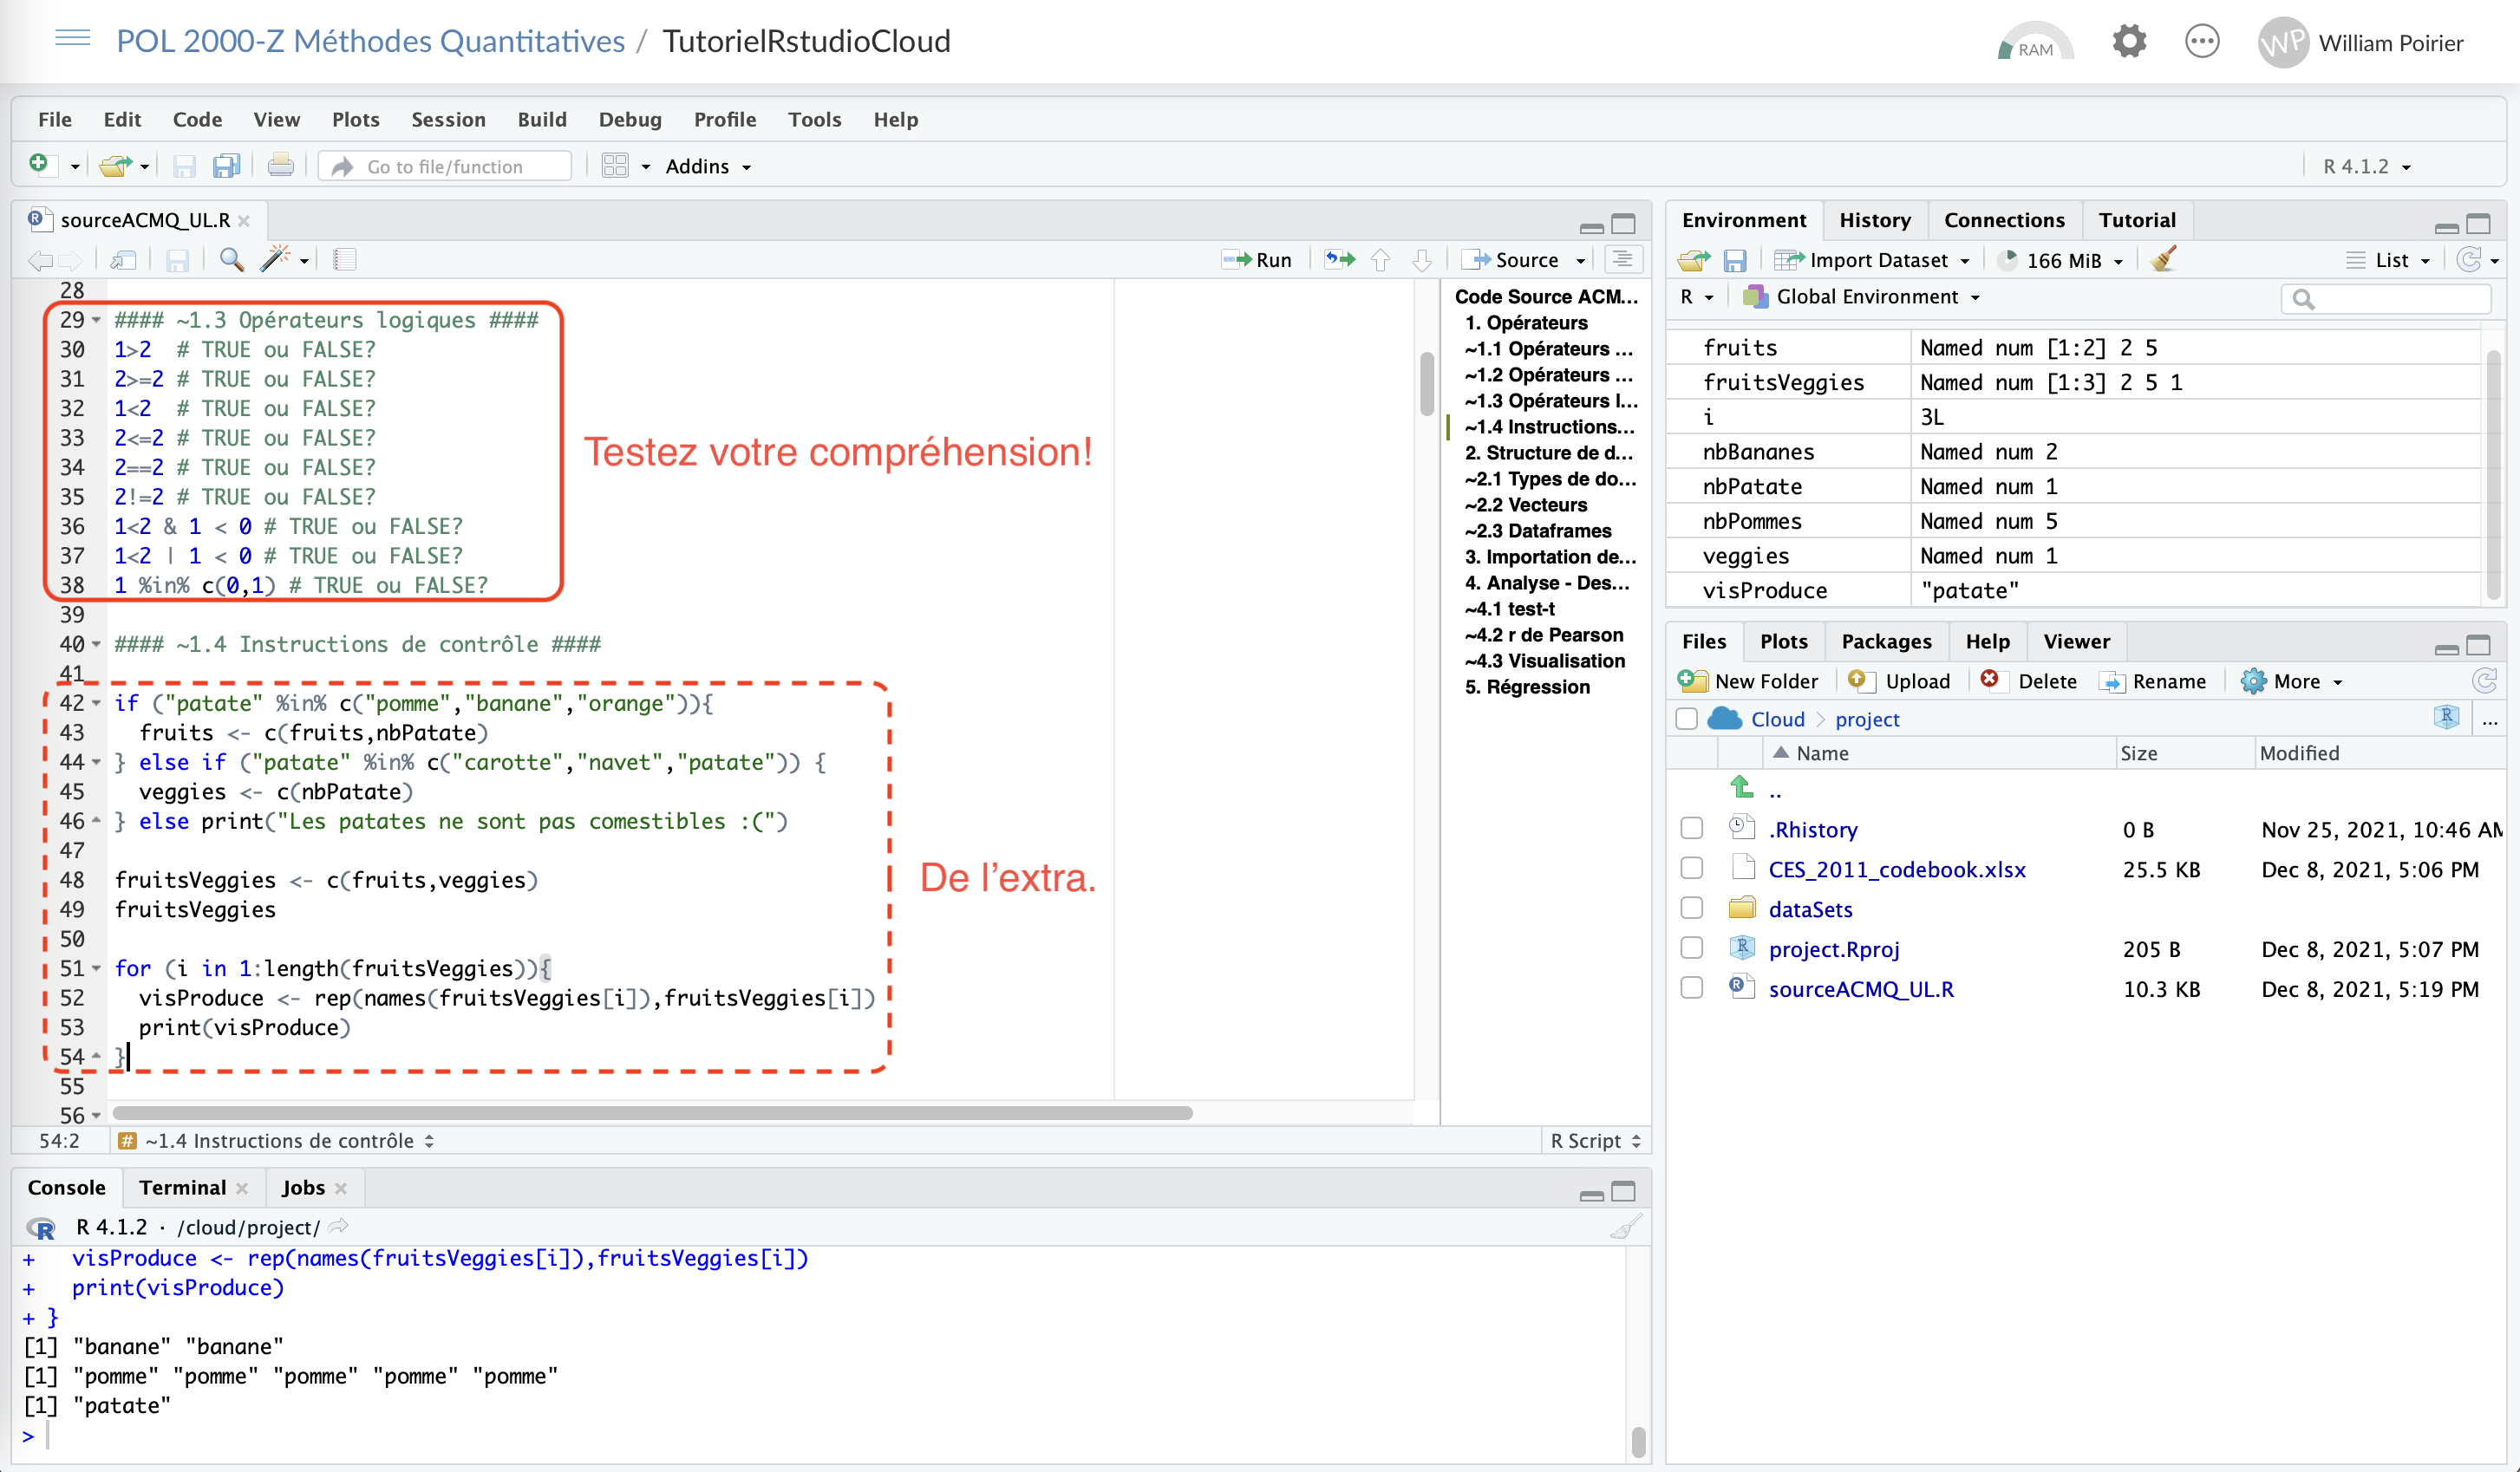
\includegraphics[width=0.98\linewidth]{_graphs/opeLogi.png}}
    \caption{Opérateurs logiques}
    \label{opeLogi}
    \end{figure}
    
    \begin{figure}[H]
    \centering
    \fbox{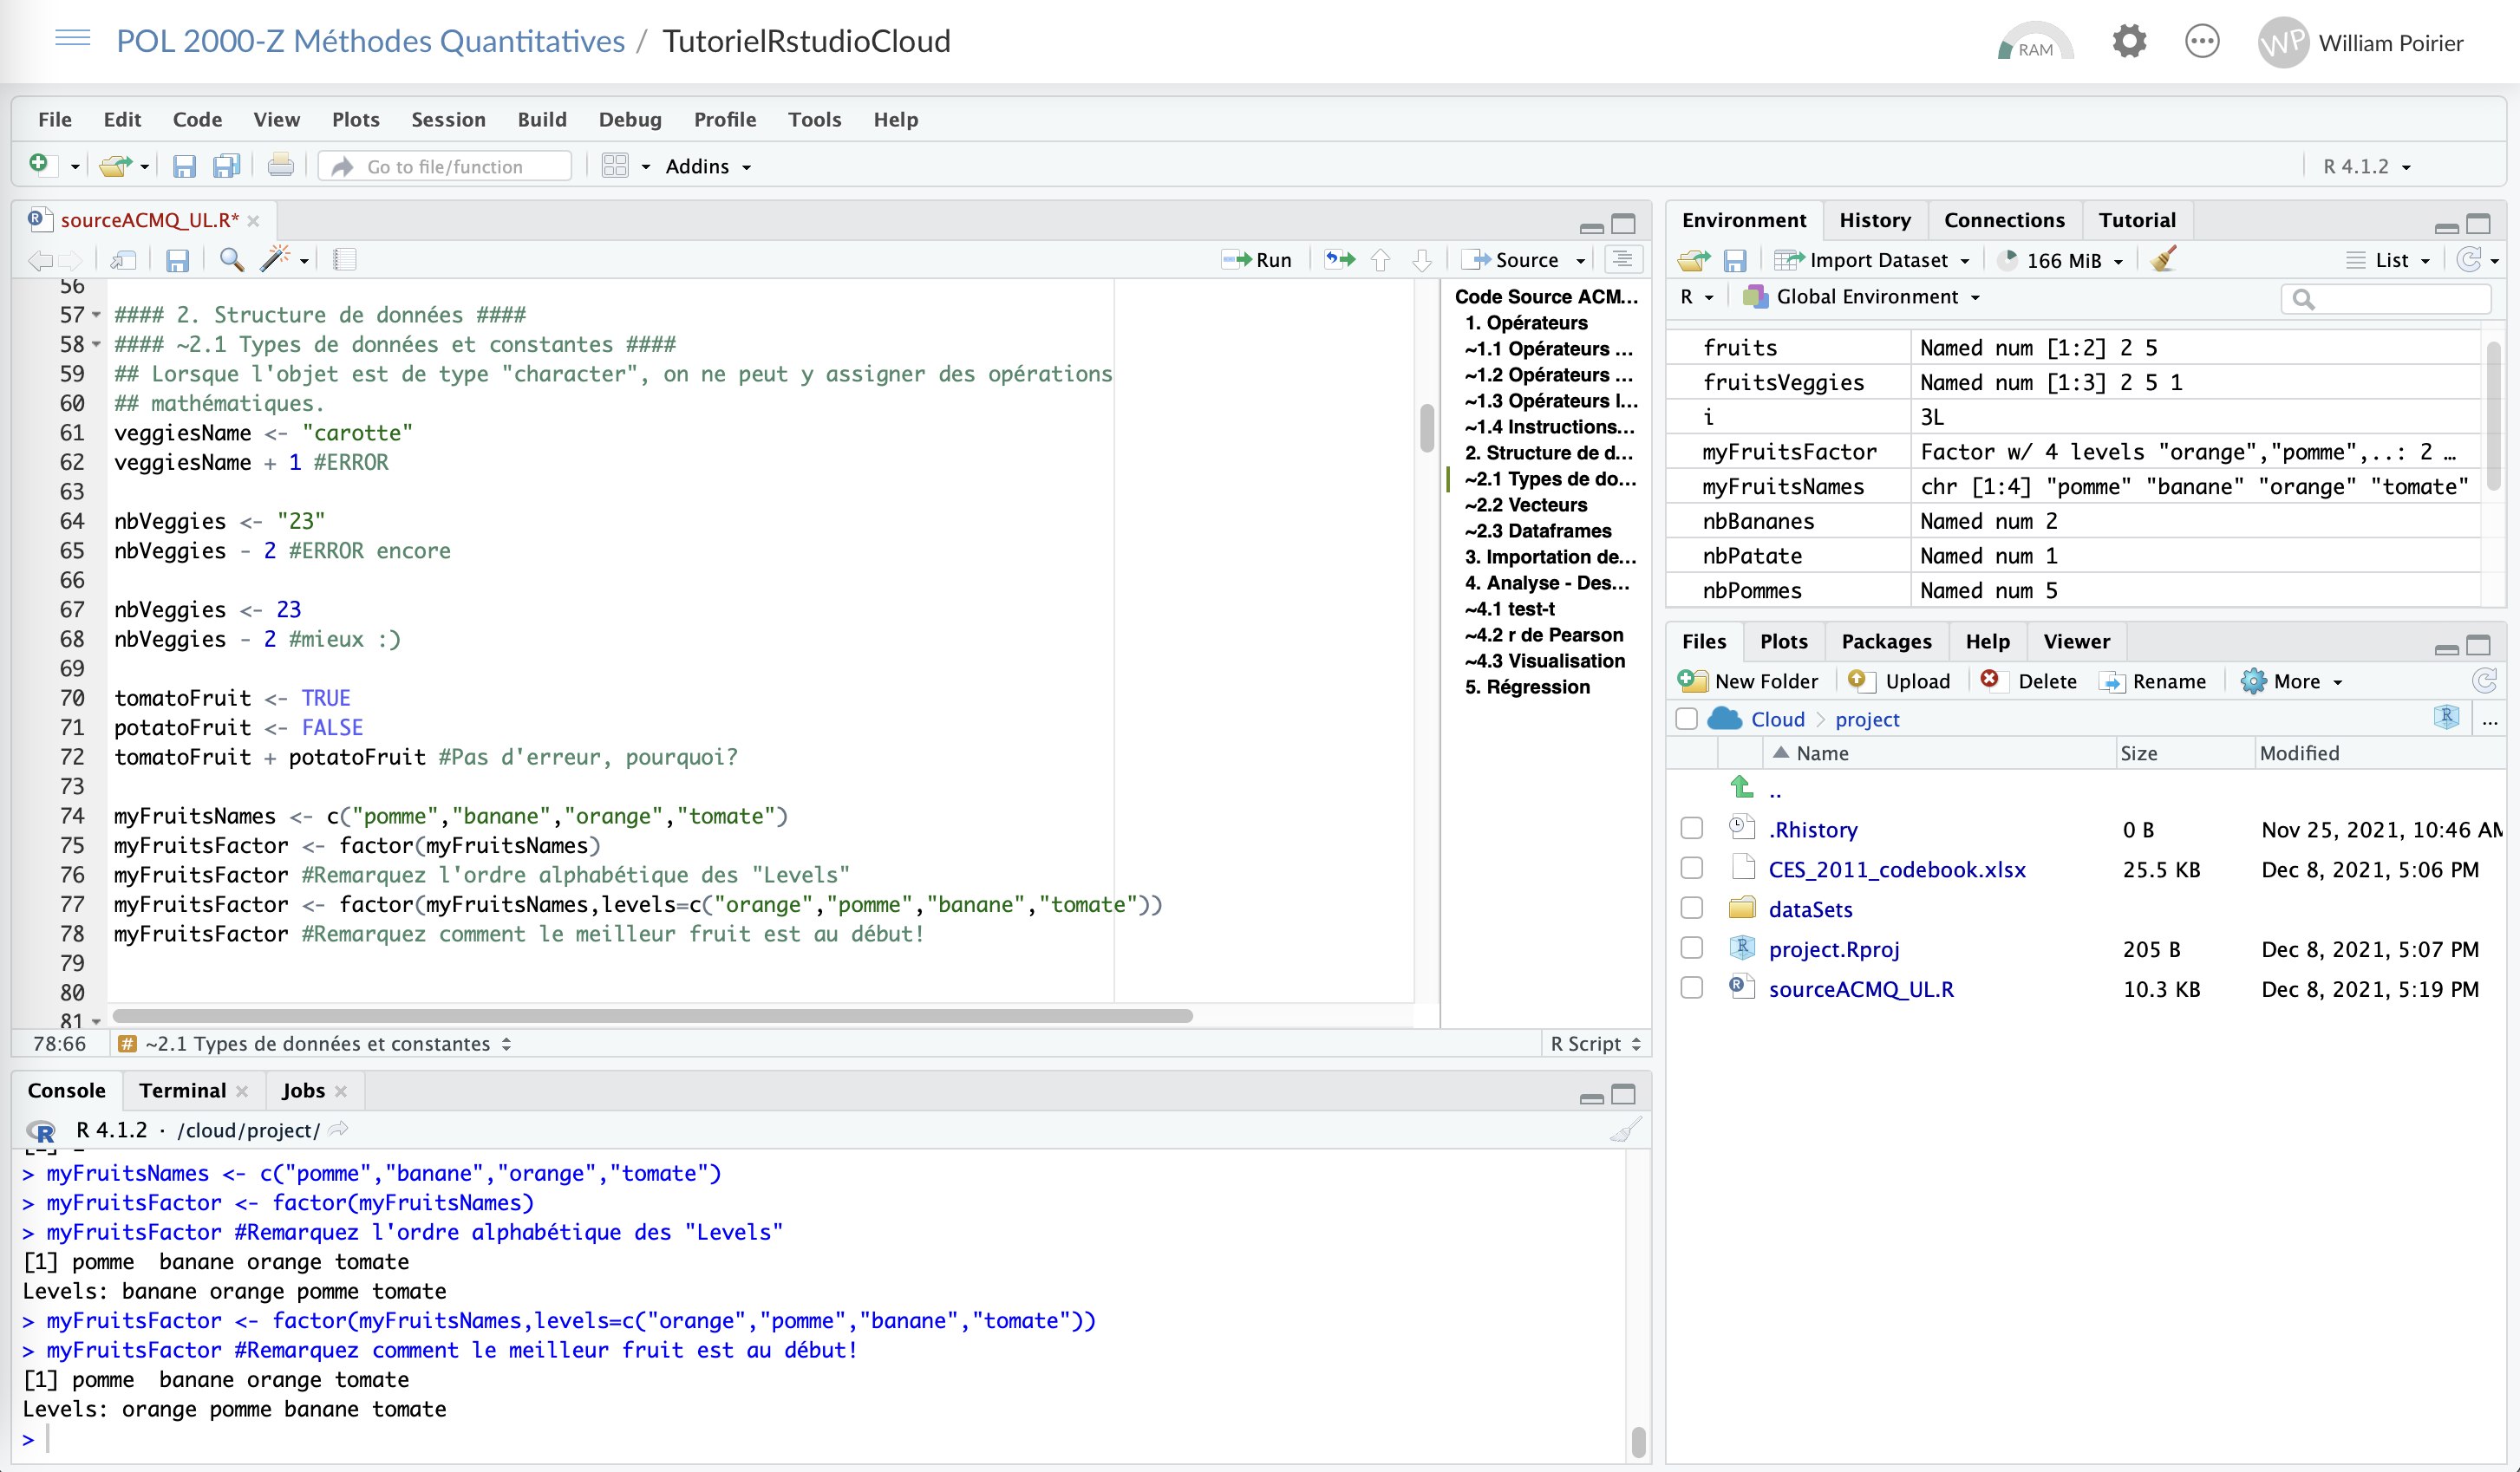
\includegraphics[width=0.98\linewidth]{_graphs/struObj.png}}
    \caption{Assigner un objet}
    \label{struObj}
    \end{figure}
    
    \begin{figure}[H]
    \centering
    \fbox{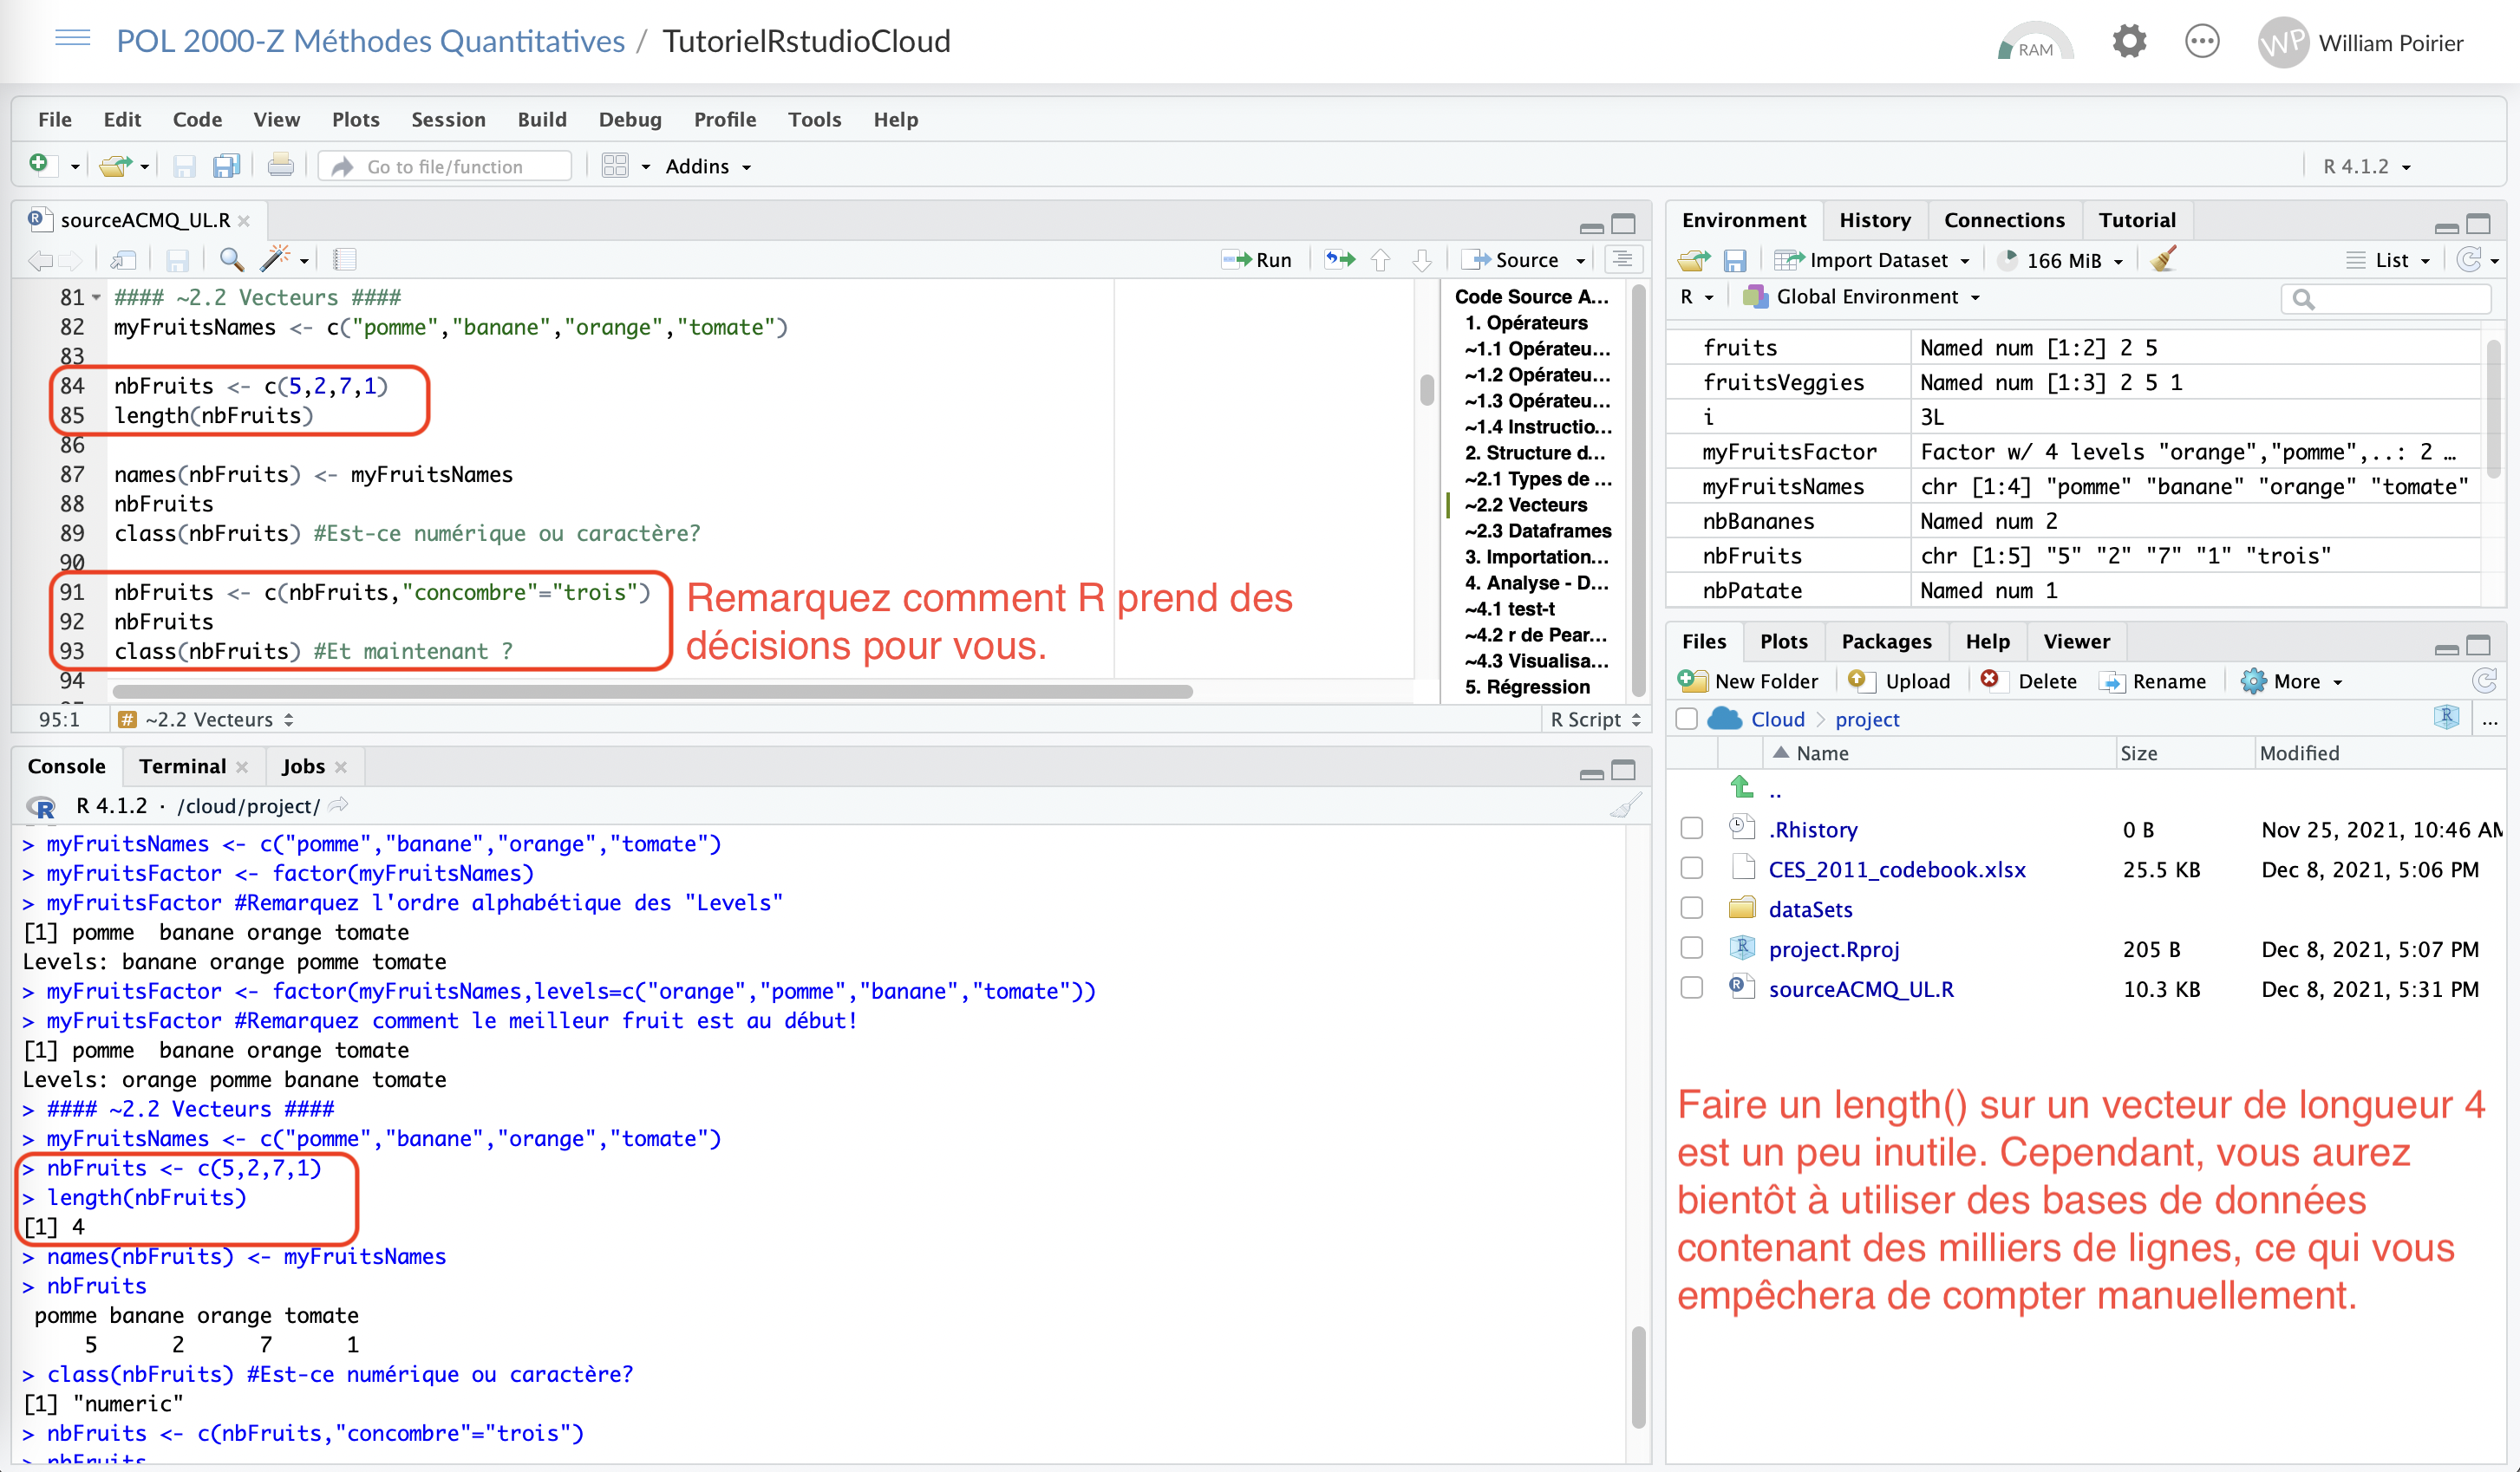
\includegraphics[width=0.98\linewidth]{_graphs/struVec1.png}}
    \caption{Le vecteur}
    \label{struVec1}
    \end{figure}
  
  \subsection{Structure de données}
  Vous savez désormais comment effectuer des opérations de base sur des objets. Or, pour ce faire, il vous faut des objets à exploiter. Ces objets peuvent prendre plusieurs formes ayant chacune des caractéristiques et fonctionnalités différentes qui les rendent plus ou moins adaptés à différent type d'utilisation. Vous verrez ici les trois formats principaux qui seront utilisés dans le cours. 
  
    \subsubsection{Types de données et constantes}
    Quatre types de données principales sont à maîtriser. Les données de classe \emph{caractère} (ou «\emph{character}») sont considérées comme du texte par \textbf{R}. \emph{Elles ne peuvent donc pas être sujettes aux opérations mathématiques standards}. Par exemple, la figure \ref{struObj} présente l'objet \rcode{veggiesName} qui contient la valeur textuelle \emph{carotte}. Pour assigner une donnée textuelle, il faut l'encadrer de guillemets « "" ». Si vous exécutez la ligne 62, vous obtiendrez une erreur puisque l'opération demandée ne peut pas s'appliquer à la classe de l'objet. Chose importante, même s'il s'agit d'un chiffre, si vous l'encadrez de guillemets comme à la ligne 64, \textbf{R} considérera l'objet comme du texte et la même erreur se produira. 
    
    Pour faire des opérations mathématiques, il faut utiliser des valeurs numériques ou booléennes. Les valeurs numériques sont des chiffres. Ceci inclut les nombres entiers, rationnels ($\pi$ ou $e$), et décimaux. Les valeurs booléennes ont deux valeurs possibles qui correspondent aux réponses possibles des opérateurs logiques, soit \rcode{FALSE} ou \rcode{TRUE}. Bien qu'à première vue les valeurs booléennes ressemblent à des données textuelles, \textbf{R} les comprend comme 0 et 1 respectivement. C'est pourquoi si on additionne \rcode{tomatoFruit} et \rcode{potatoFruit}, on obtient 1. Pour ceux et celles d'entre vous un peu confus par ceci, rappelez-vous du processus de la codification des données et des guides de référence pour expliquer les bases de données.
    
    Un format alternatif et particulier des données textuelles et numériques est le \emph{facteur}. Conceptuellement, un facteur en \textbf{R} est un objet pouvant prendre un nombre limité de valeurs. En d'autres mots, il s'agit d'une variable catégorielle. À ces valeurs il est possible d'imposer un ordre (pensez ici aux variables ordinales, intervalles et ratio). Par défaut, \textbf{R} ordonnera les valeurs numériques en ordre croissant et les valeurs textuelles en ordre alphabétique. En utilisant la fonction \rcode{factor()}, il est possible de créer un objet de classe facteur et de lui imposer un ordre avec l'argument \emph{levels}. Si les facteurs vous semblent compliqués pour rien, ils vous seront très utiles lorsque vous voudrez faire de la visualisation de données plus avancée. Il s'agit également d'une source d'erreur importante. Assurez-vous donc de bien connaître la classe des objets avec laquelle vous travaillez.
    
    Il est possible de connaître la classe d'un objet en regardant ce qui se trouve à l'intérieur. Or, ce n'est pas toujours possible ou évident, soit à cause de la taille de l'objet (la quantité de choses qui s'y trouve), soit parce qu'on peut confondre un 1 caractère et un 1 numérique ou une "pomme" caractère et une "pomme" facteur. Pour être absolument certain, il est toujours préférable de demander à \textbf{R} en utilisant la fonction \rcode{class()}.
    
    Les constantes sont des objets avec une seule donnée d'associée. À la figure \ref{struObj}, \rcode{veggiesName}, \rcode{nbVeggies}, et \rcode{tomatoFruit} sont des constantes, un objet avec un seul élément. Ces constantes n'ont cependant pas la même classe -- soit, respectivement, caractère, numérique et booléen. Les constantes forment l'unité de base des structures de données possibles en \textbf{R}.
    
    \subsubsection{Vecteurs}\label{vec}
    Vous avez sans doute déjà entendu parler de vecteurs dans vos cours de mathématiques au secondaire. N'ayez crainte, il n'est pas question de la même chose ici. Un vecteur, pour \textbf{R}, c'est une série de données du même type. En d'autres mots, c'est une suite de constantes de la même classe mises bout à bout. Un vecteur \textbf{R} peut également être compris comme contenant les valeurs d'une variable -- des notes d'examen, le positionnement idéologique, ou des noms de fruits. Sans vecteur, il n'est pas possible pour \textbf{R} d'effectuer des opérations aussi simples que le calcul d'une moyenne. Autant dire que \textbf{R} ne sert pas à grand chose sans vecteur. Heureusement, vous en avez déjà rencontré sans l'avoir remarqué. À la figure \ref{struVec1}, \rcode{myFruitsNames} est un vecteur de classe « caractère » et de longueur 4. Pour déterminer combien d'éléments contient un vecteur (ou quelle est sa longueur, vous pouvez les compter vous-même ou demander à \textbf{R} de le faire pour vous avec la fonction \rcode{length()} comme c'est fait à la ligne 85 de la figure \ref{struVec1}. 
    
    Pour créer un vecteur, il faut utiliser la fonction \rcode{c()} et l'assigner à un objet, comme à la ligne 82 de la figure \ref{struVec1}. Le \rcode{c} de la fonction représente le verbe anglais «concatenate» qui signifie relier beaucoup de choses ensemble dans une chaîne ou une série. Vous pouvez également ajouter des noms aux éléments de votre vecteur. Ces noms n'auront aucune influence sur le traitement des valeurs associées. Par exemple, à la figure \ref{struVec1}, j'ai un vecteur avec le nombre de chaque type de fruits dans le bon ordre (\rcode{nbFruits}). Si je désire leur associer un nom pour ne pas oublier ce que chaque chiffre représente, je peux utiliser la fonction \rcode{names()} comme à la ligne 87 de la figure \ref{struVec1}. Cette ligne se lit comme suit : aux noms des éléments de \rcode{nbFruits}, assigne les valeurs qui se trouvent dans \rcode{myFruitsNames}. Vous pouvez également associer directement les noms de chaque élément à la création du vecteur comme à la ligne 91 de la figure \ref{struVec1}. 
    
    À la ligne 91 de la figure \ref{struVec1}, j'amende le vecteur \rcode{nbFruits} en y ajoutant un élément. Remarquez comment je réutilise l'objet \rcode{nbFruits} dans l'opération. La ligne 91 se lit : associe à l'objet \rcode{nbFruits} un vecteur des valeurs déjà contenues dans \rcode{nbFruits} et la valeur "trois" au nom "concombre". Or, n'ai-je pas dit plus haut qu'un vecteur se devait d'avoir le même type de valeurs? \textbf{R} est gentil, il vous laisse le faire sans retourner d'erreur. À la place, il prend une décision pour vous en assignant la classe caractère à \textbf{TOUS} les éléments du nouveau vecteur. C'est donc important d'être attentif à ce que fait \textbf{R}; il prend parfois de mauvaises décisions pour vous. 
    
    Lorsque le vecteur est de classe numérique, il est possible d'effectuer des opérations mathématiques plus ou moins complexes. Vous pouvez bien sûr additionner, soustraire, multiplier et diviser par la même valeur tous les éléments du vecteur. Or, \textbf{R} vous permet aussi d'effectuer les opérations statistiques de base sans appel à d'autres librairies. La moyenne, la médiane, l'écart-type, la variance et plusieurs autres opérations ont des fonctions associées. Vous pouvez les consulter à la figure \ref{struVec2}. Je vous encourage à explorer le code et à expérimenter. 
    
    Le dernier élément important à aborder au sujet des vecteurs est la façon de sélectionner des éléments. Pour ce faire, on utilise les crochets "[]". Ceux-ci nous permettent d'indiquer la position dans le vecteur des éléments à sélectionner. La figure \ref{struVec2} montre, dans l'ordre à partir de la ligne 117, comment sélectionner un élément, une suite d'éléments et plusieurs éléments distincts. Il est également possible d'apposer un \rcode{-} devant le chiffre pour retirer l'élément. 
    
    \begin{figure}[H]
    \centering
    \fbox{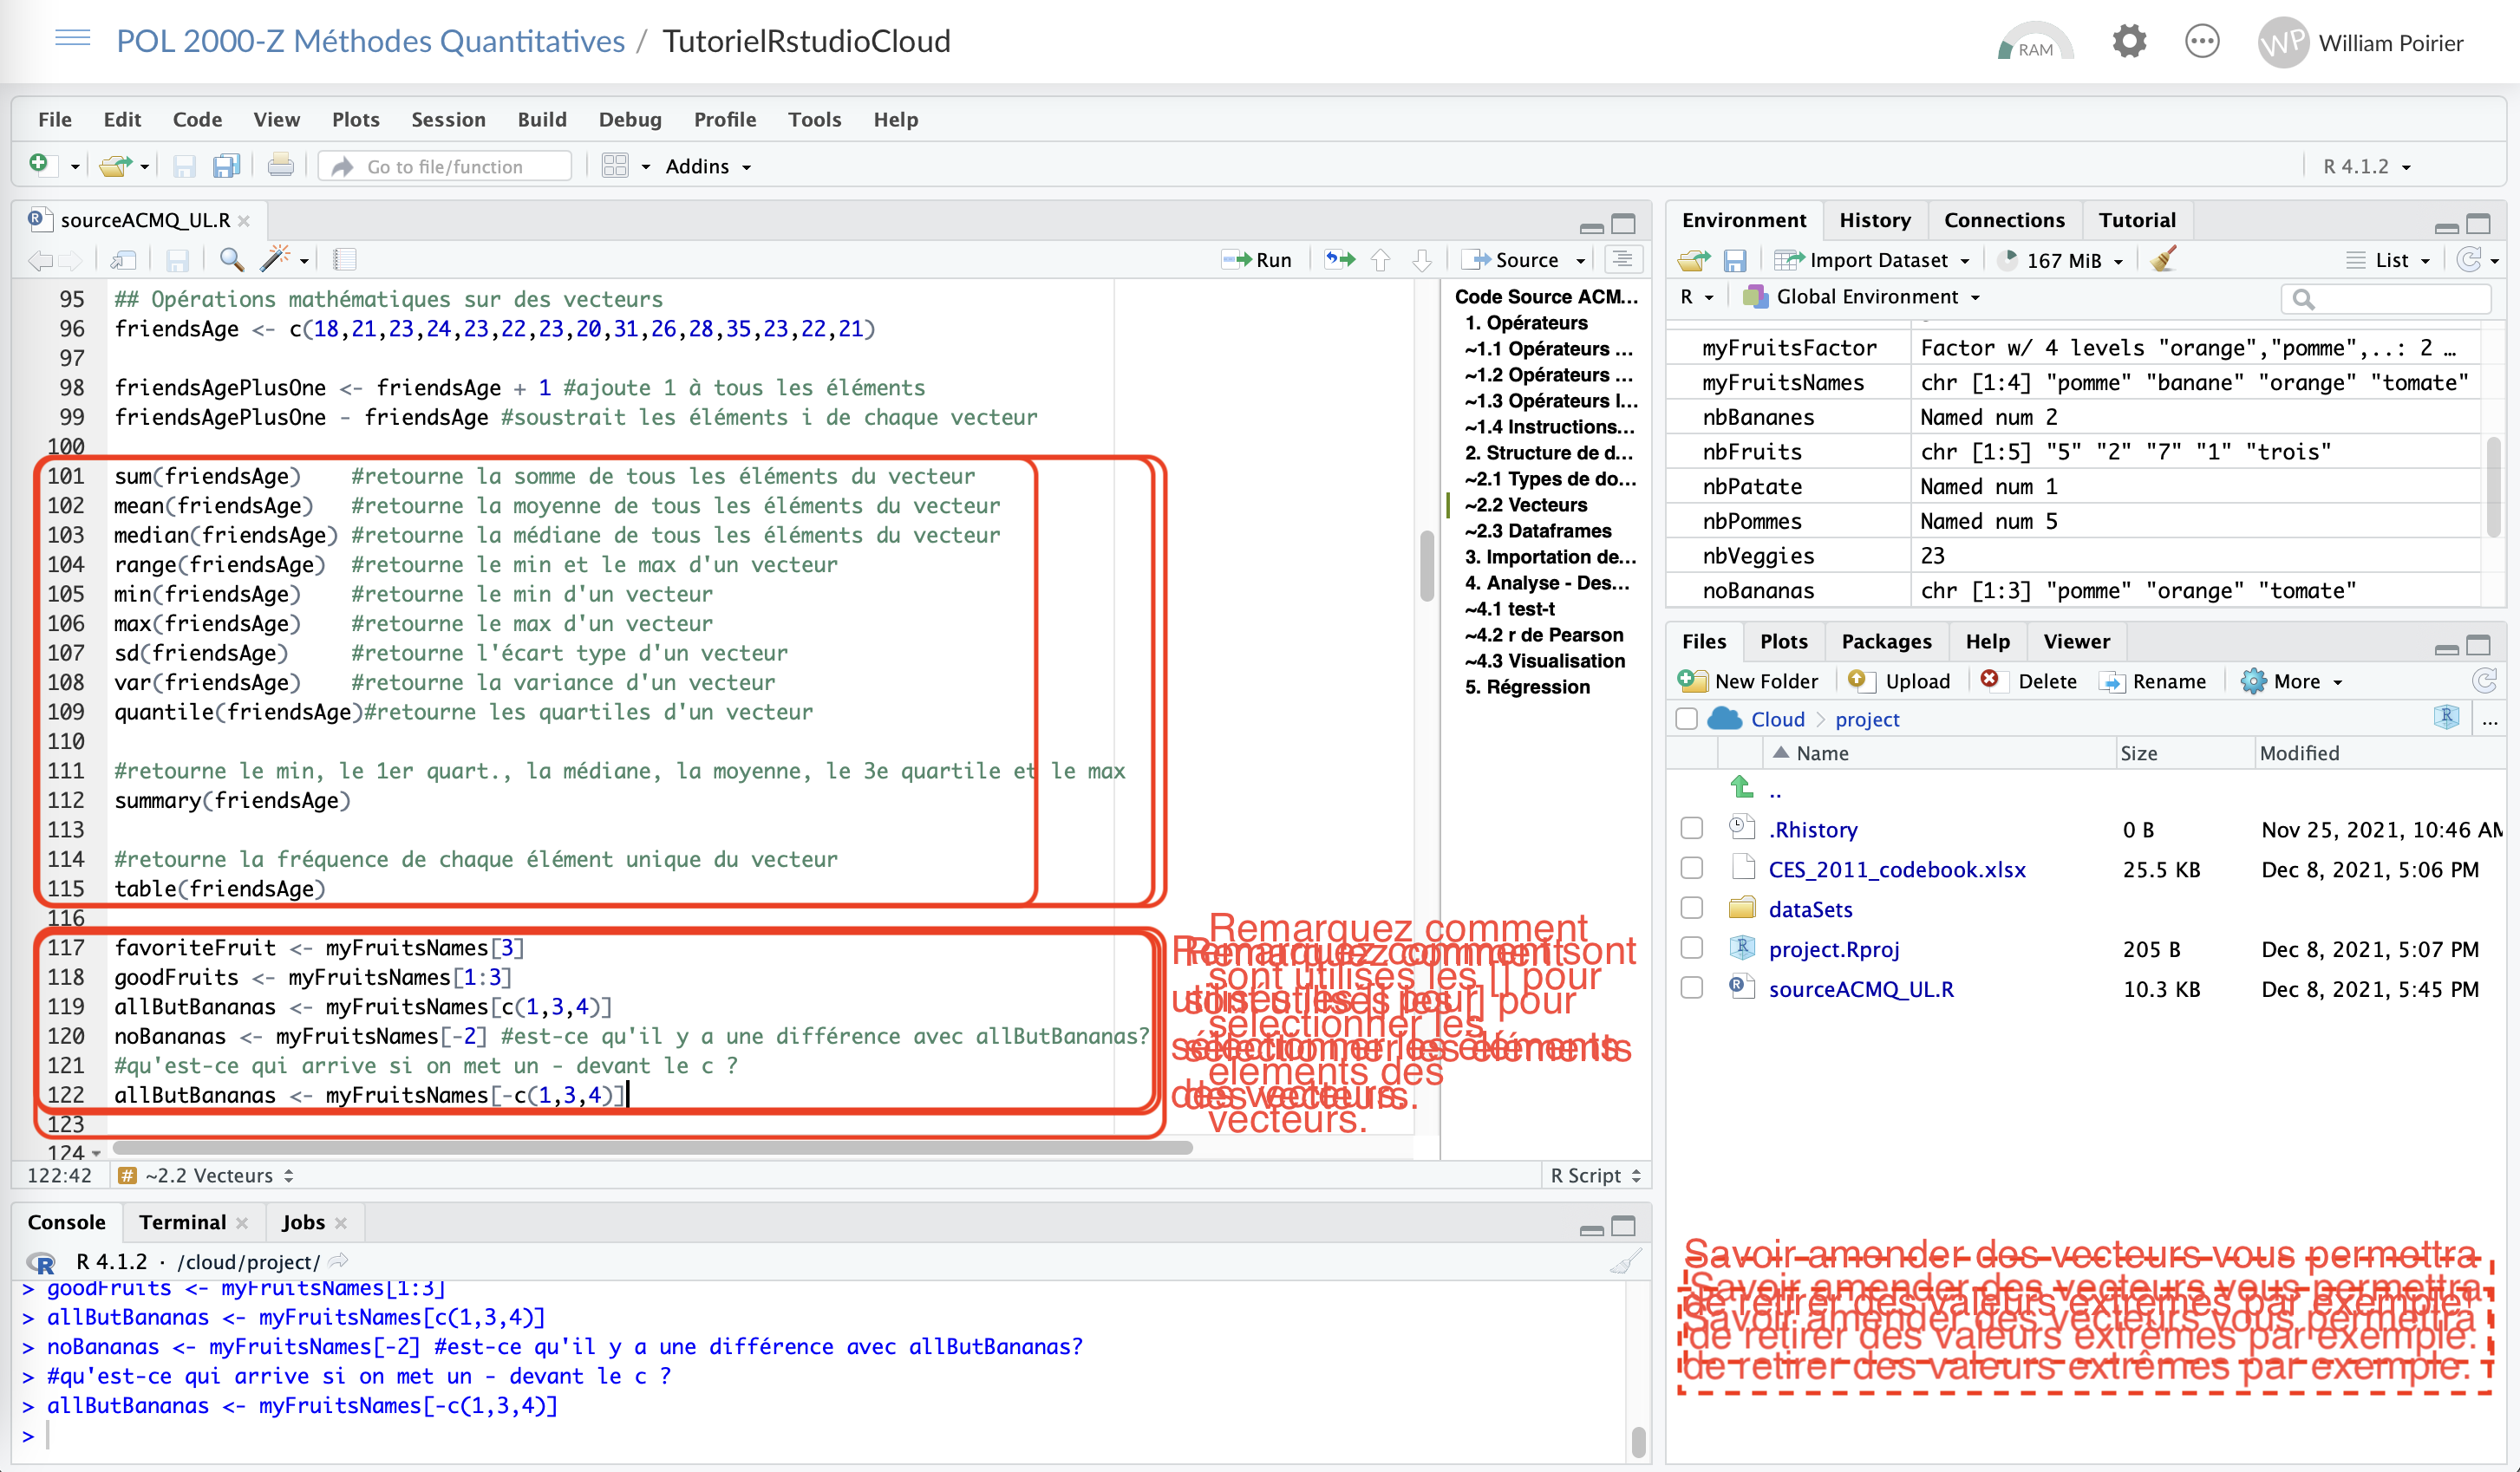
\includegraphics[width=0.98\linewidth]{_graphs/struVec2.png}}
    \caption{Opérations mathématiques de base}
    \label{struVec2}
    \end{figure}
    
    \begin{figure}[H]
    \centering
    \fbox{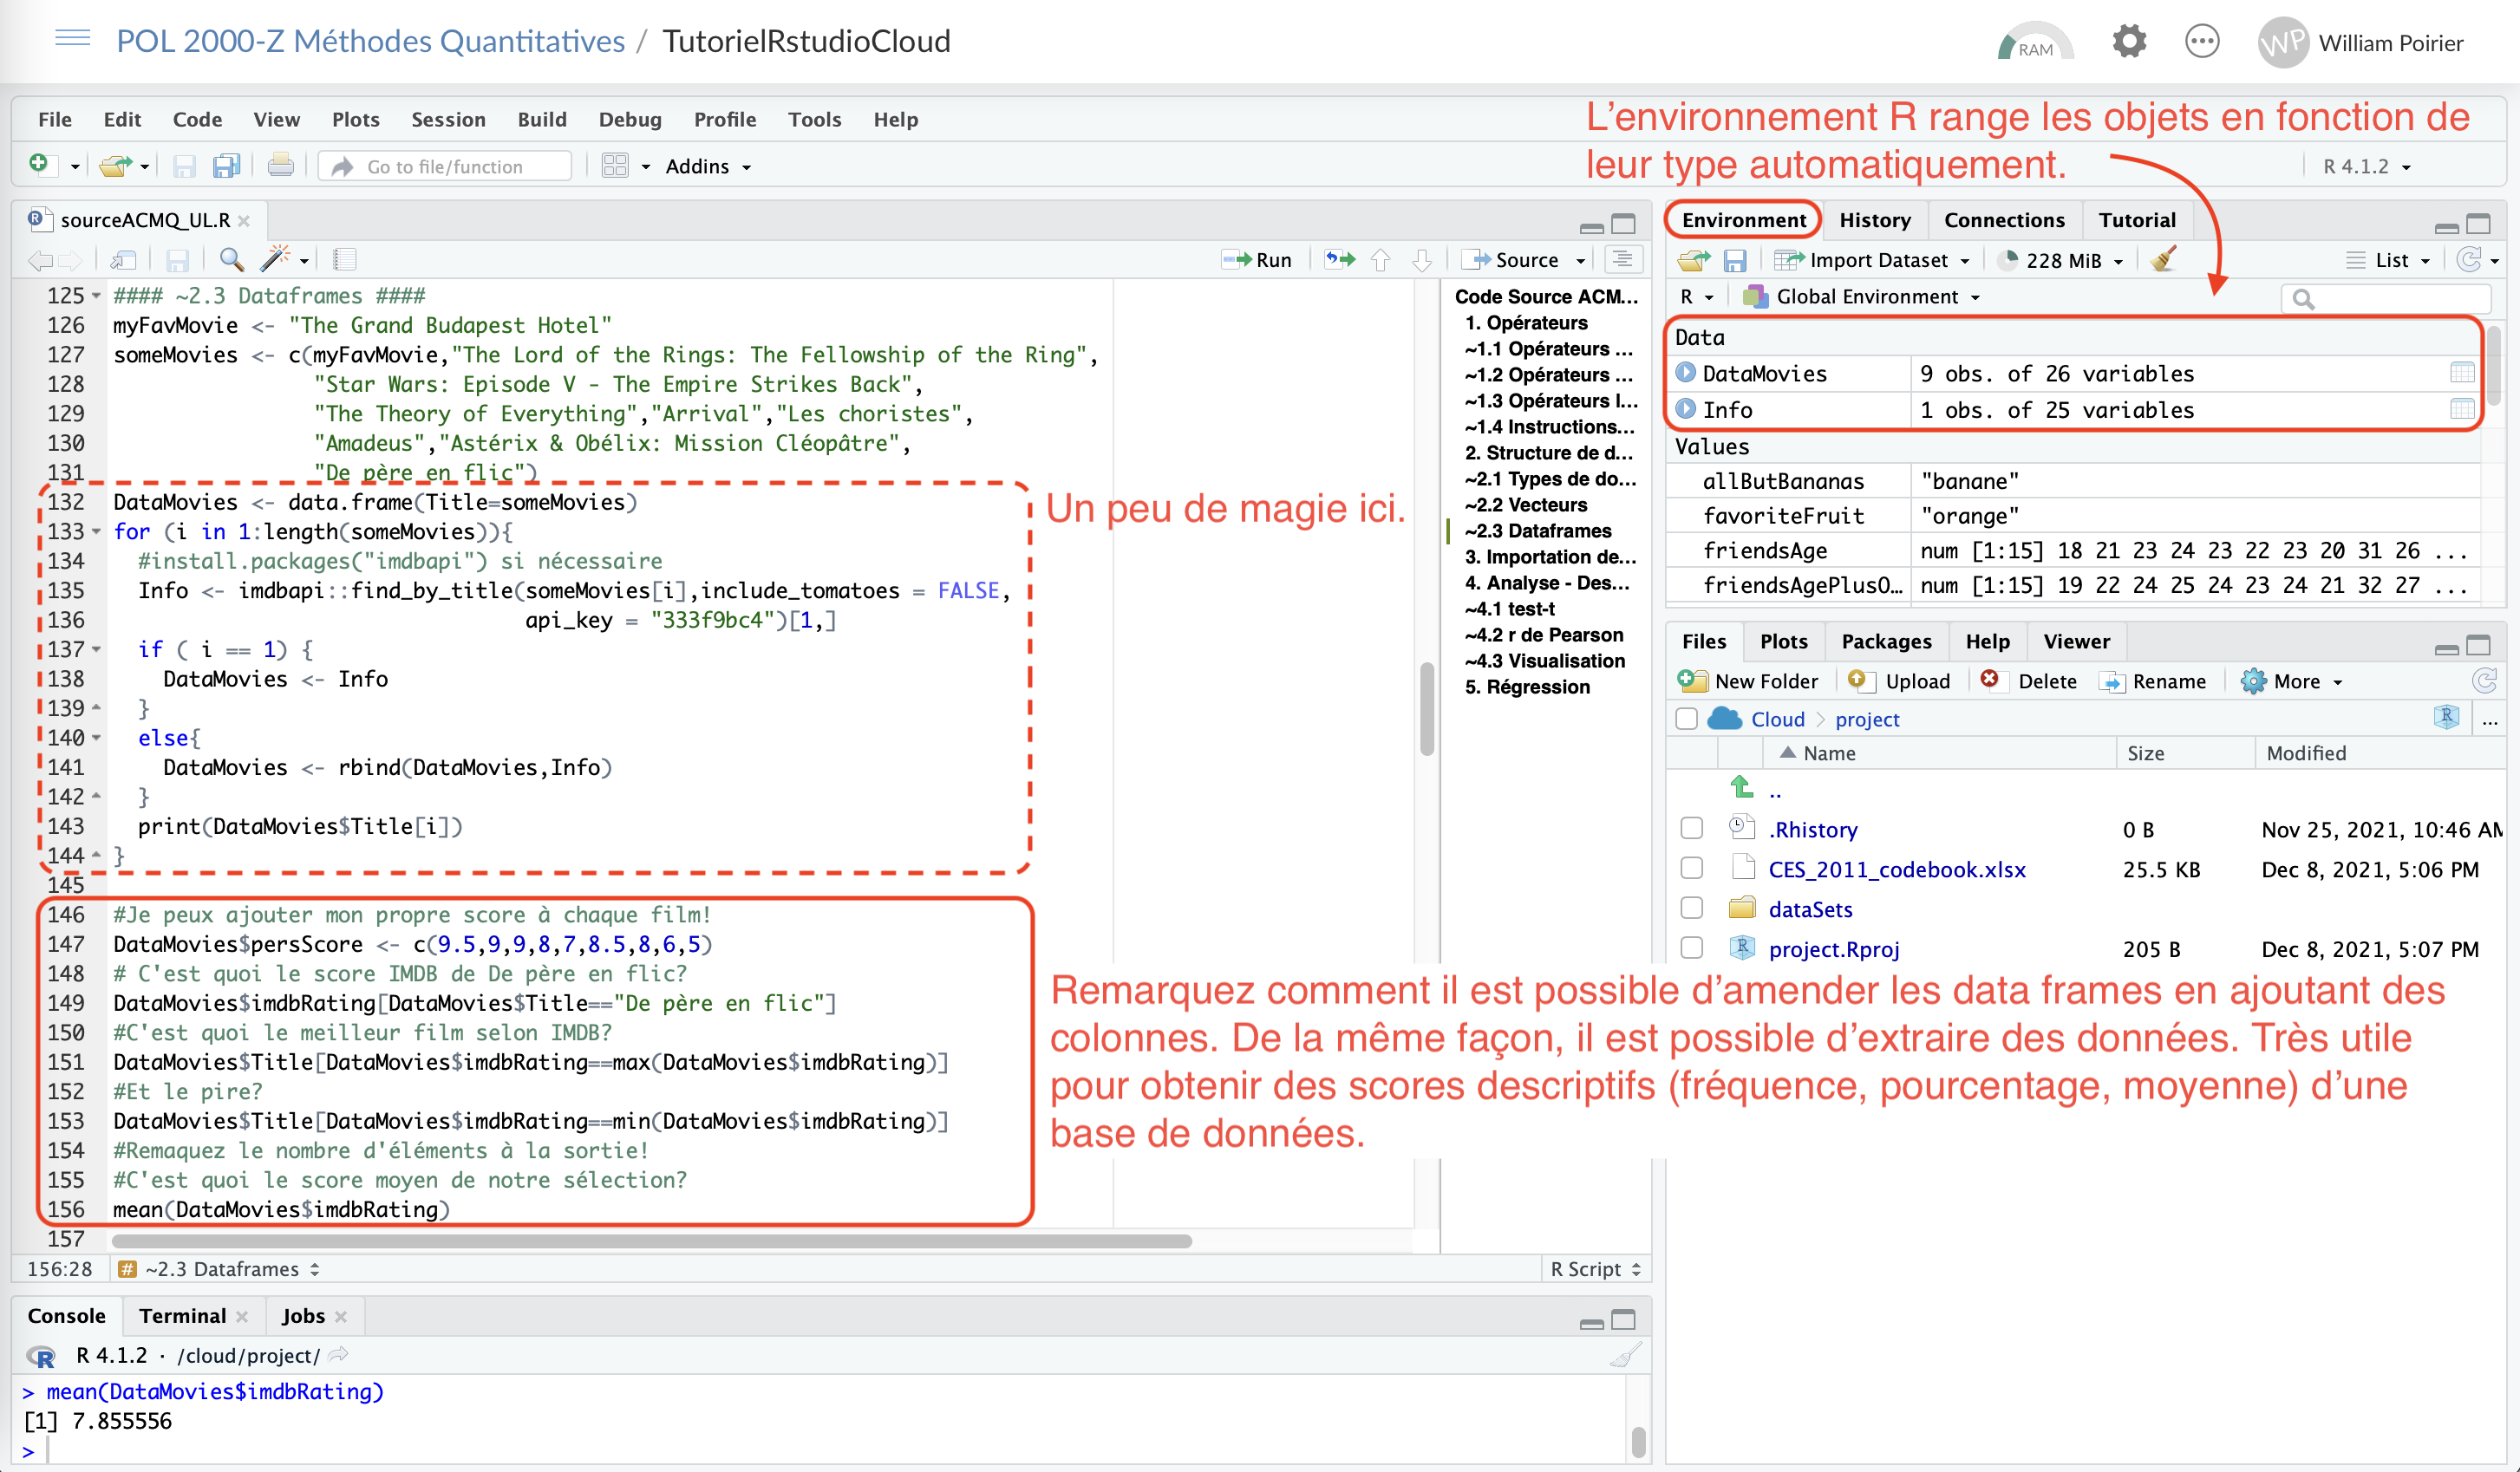
\includegraphics[width=0.98\linewidth]{_graphs/struDataF.png}}
    \caption{Le \emph{data frame}}
    \label{struDataF}
    \end{figure}
    
    
    \subsubsection{Data frames}
    
    \begin{wrapfigure}{r}{0.5\linewidth}
      \centering
      \fbox{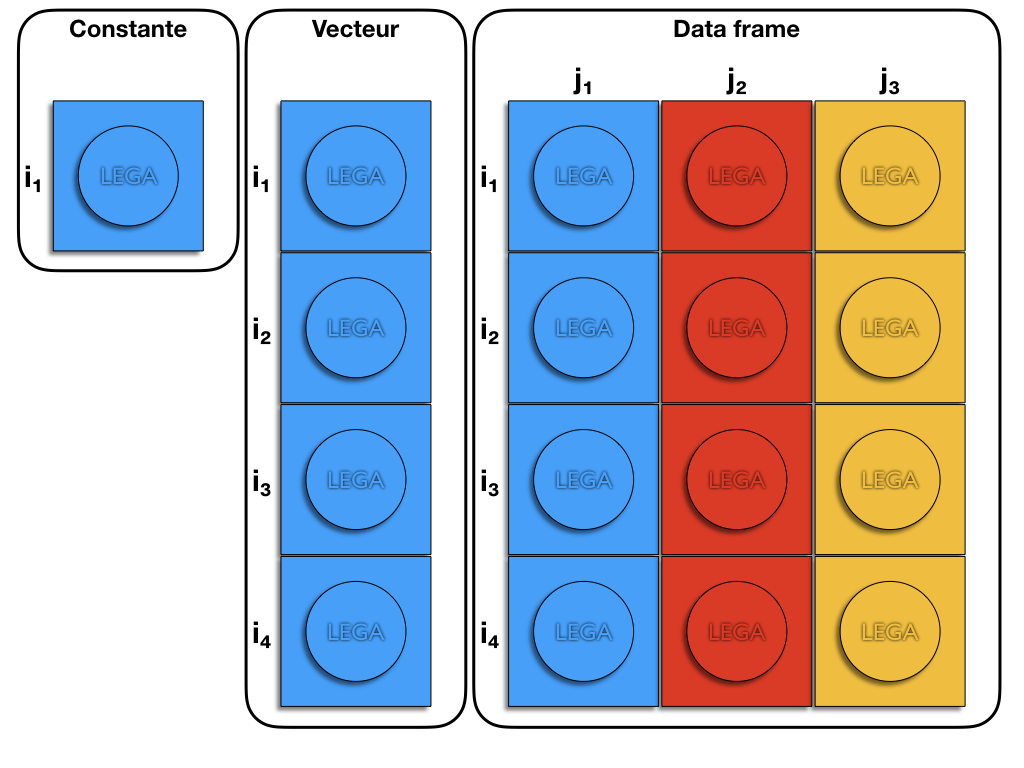
\includegraphics[width=1\linewidth]{_graphs/lego.png}}
      \caption{Représentation des types d'objets \textbf{R}}
      \label{lego}
    \end{wrapfigure}
    
    Un \emph{data frame} (il n'y a pas vraiment de traduction satisfaisante, mais le terme base de données est aussi communément utilisé) contient des données organisées en rangées et en colonnes, comme un tableau Excel. Chaque colonne peut avoir une classe différente, mais les données au sein d’une même colonne doivent être de la même classe. \emph{Généralement, les colonnes seront associées aux variables, tandis que chaque rangée correspondra à une observation.}
    
    Les \emph{data frames} sont composés de vecteurs de la même façon que les vecteurs sont composés de constantes. On peut donc avoir un film préféré (une constante), une liste de films que nous avons vus (un vecteur) ainsi qu'un fichier Excel regroupant ces films, leur année de publication, leur genre, leur score IMDB, etc.\footnote{Vous remarquerez que je fais appel au \emph{package} \rcode{imdbapi} à la figure \ref{struDataF}. Il s'agit d'une librairie contenant des fonctions qui me permettent de communiquer avec l'API d'IMDB et de lui faire des requêtes. Dans le code, je fournis une clé pour y accéder, mais pour celles et ceux qui désireraient leur propre clé c'est \href{http://www.omdbapi.com/apikey.aspx}{ici} $\mapsto$ \href{http://www.omdbapi.com/apikey.aspx}{http://www.omdbapi.com/apikey.aspx}. Pour de la documentation sur le package c'est \href{https://cran.r-project.org/web/packages/imdbapi/imdbapi.pdf}{là} $\mapsto$ \href{https://cran.r-project.org/web/packages/imdbapi/imdbapi.pdf}{https://cran.r-project.org/web/packages/imdbapi/imdbapi.pdf}.} Bien qu'il soit possible de créer des \emph{data frames} par vous-même, il est rare qu'un chercheur construise manuellement sa base de données directement dans \textbf{R}. Le plus souvent, une base de données existante est téléchargée ou créée dans d'autres logiciels comme un fichier Excel. 
    
    Comme les constantes et les vecteurs sont à la base du fonctionnement de \textbf{R}, le \emph{data frame} est l'objet le plus important pour le travail des analystes de données. En effet, les données que vous analyserez ne viendront pas sous forme de vecteur, ce serait un cauchemar d'organisation. Imaginez avoir à calculer la moyenne d'un.e étudiant.e pour un cours avec 20 évaluations. Créer un vecteur avec les notes de tous les étudiant.es pour chaque évaluation serait beaucoup trop inefficace. La solution serait de créer un fichier Excel avec une colonne pour les noms des étudiant.es et une colonne par évaluation. Ainsi, au lieu d'avoir 20 vecteurs nommés (rappelez-vous de la fonction \rcode{names()} à la figure \ref{struVec1}), vous auriez 1 fichier avec 21 colonnes. Ceci vous permet non seulement de calculer la moyenne par étudiant, mais également de croiser vos données. Par exemple, vous pourriez ajouter l'âge des étudiant.es ou leur nombre de sessions universitaires complétées afin d'évaluer si l'une de ces variables semble avoir un effet sur la réussite du cours. C'est ici que la puissance de \textbf{R} peu vraiment être exploitée, et c'est pourquoi il est très important de bien comprendre comment manipuler le \emph{data frame}. Il en va de votre capacité à analyser les données. Les prochains paragraphes pourront paraître plus obtus, mais il faut faire un effort pour bien les comprendre. 
    
    %Pour créer des \emph{data frames}, on utilise la fonction \rcode{data.frame()} comme à la ligne 132 de la figure \ref{struDataF}. Ici, je crée un \emph{data frame} de 9 rangées (le nombre d'éléments du vecteur \rcode{someMovies}) avec une seule colonne nommée \emph{Title}. Il est possible de créer un \emph{data frame} avec autant de colonnes que l'on désire, on a qu'à ajouter des vecteurs (en les séparant de virgules) à la fonction \rcode{data.frame()} lors de la création. Cependant, il est rare qu'un chercheur construise manuellement sa base de données directement dans \textbf{R}. Le plus souvent se sera fait dans un fichier Excel au préalable ou à partir de différents logiciels (\textit{Qualtrics} pour faire des sondages par exemple). Dans le cas de la figure \ref{struDataF}, j'utilise un API pour créer mon propre \emph{data frame}. C'est une technique plus avancée qui va au\-/delà du cours.
    
    %Une fois votre \emph{data frame} créé ou importé (ce que nous verrons à la section \ref{import}), il possible d'effectuer différentes opérations similaires à ce que nous avons vu pour les vecteurs. 
    L'aspect important à reconnaître, c'est qu'un \emph{data frame} a deux dimensions au lieu d'une (les rangées et les colonnes). Pour se déplacer dans un \emph{data frame}, il faut donc ajouter un élément à nos crochets (\rcode{[]}) habituel. Dans \textbf{R}, le premier élément retrouvé dans les crochets correspond au numéro de la rangé, le second au numéro de la colonne. Essentiellement les r et les c de la figure \ref{lego}. Bien que \textbf{R} soit un outil puissant, il nous demande souvent de faire des abstractions, comme d'indiquer exactement la rangée et la colonne qui nous intéresse. Une manière de visualiser ceci est d'imaginer un fichier Excel ou un jeu d'échecs qui vous indique les colonnes avec des lettres et les rangées avec des chiffres. Ainsi, si je m'intéresse au deuxième élément de la troisième colonne d'un \emph{data frame} nommé \rcode{Data}, je peux l'extraire avec \rcode{Data[2,3]}. Une erreur que font plusieurs codeurs est d'inverser rangées et colonnes. Il faut se souvenir: rangé, colonne, ou \rcode{Data[r,c]}!
    
    Il est cependant rare que nous nous intéressions à des colonnes ou à des cellules particulières d'un \emph{data frame} en termes de numéros de rangée et de colonne. Le plus souvent, nous voulons faire une opération sur une colonne comme une moyenne afin d'avoir des statistiques descriptives. À la figure \ref{struDataF}, nous nous intéressons à la moyenne des scores IMDB d'une sélection de films. Pour ce faire, nous utilisons le \rcode{\$} pour dire à \textbf{R} que nous nous intéressons à la colonne \rcode{imdbRating} de \rcode{DataMovies} (\rcode{Data\$nomDeLaColonne}).
    
    De la même façon, il est également possible de combiner le \rcode{\$} avec les crochets (\rcode{[]}) pour sélectionner des éléments d'un \emph{data frame} sous certaines conditions. Ceci est un outil puissant pour explorer vos données. Dans le cas du score IMDB de «~De père en flic~», la ligne se lit : dans la colonne \rcode{imdbRating} du \emph{data frame} \rcode{DataMovies}, sélectionne les éléments dont la valeur à la même rangée dans la colonne \rcode{Title} du \emph{data frame} \rcode{DataMovies} est égale à "De père en flic". Les possibilités de conditionnalité sont donc infinies. Dans l'exemple on s'intéresse aux scores maximum et minimum, mais il est possible de combiner des tests booléens (vrai ou faux, \rcode{TRUE}/\rcode{FALSE}) avec les arguments conditionnels "\rcode{|}" (OR) et "\rcode{\&}" (AND). 
  
%    De la même façon, il est possible d'ajouter une colonne ou de modifier une colonne existante lui assignant ("->") des valeurs. C'est ce qui est fait à la ligne 147 de la figure \ref{struDataF}, j'assigne mes propres scores à notre sélection de films. Il est également possible de combiner le \$ avec les crochets ("[]") pour sélectionner des éléments d'un \emph{data frame} sous certaines conditions. Dans le cas du score IMDB de «~De père en flic~», la ligne se lit : dans la colonne \rcode{imdbRating} du \emph{data frame} \rcode{DataMovies}, sélectionne les éléments dont la valeur à la même rangée dans la colonne \rcode{Title} du \emph{data frame} \rcode{DataMovies} est égale à "De père en flic". Les possibilités de conditionnalité sont donc infinies. Dans l'exemple on s'intéresse aux scores maximum et minimum, mais il est possible de combiner des tests booléens (vrai ou faux, \rcode{TRUE}/\rcode{FALSE}) avec les arguments conditionnels \rcode{|} (OR) et \rcode{\&} (AND). 
    
    Enfin, les mêmes opérations mathématiques décrites à la figure \ref{struVec2} pour les vecteurs s'appliquent aux colonnes des \emph{data frames}. C'est normal, rappelez-vous, une colonne d'un \emph{data frame} c'est comme un vecteur. Il n'y a qu'à choisir la colonne avec le \rcode{\$} et on peut appliquer les fonctions de moyenne, d'écart-type, de variance, etc.
    
    \begin{figure}[H]
    \centering
    \fbox{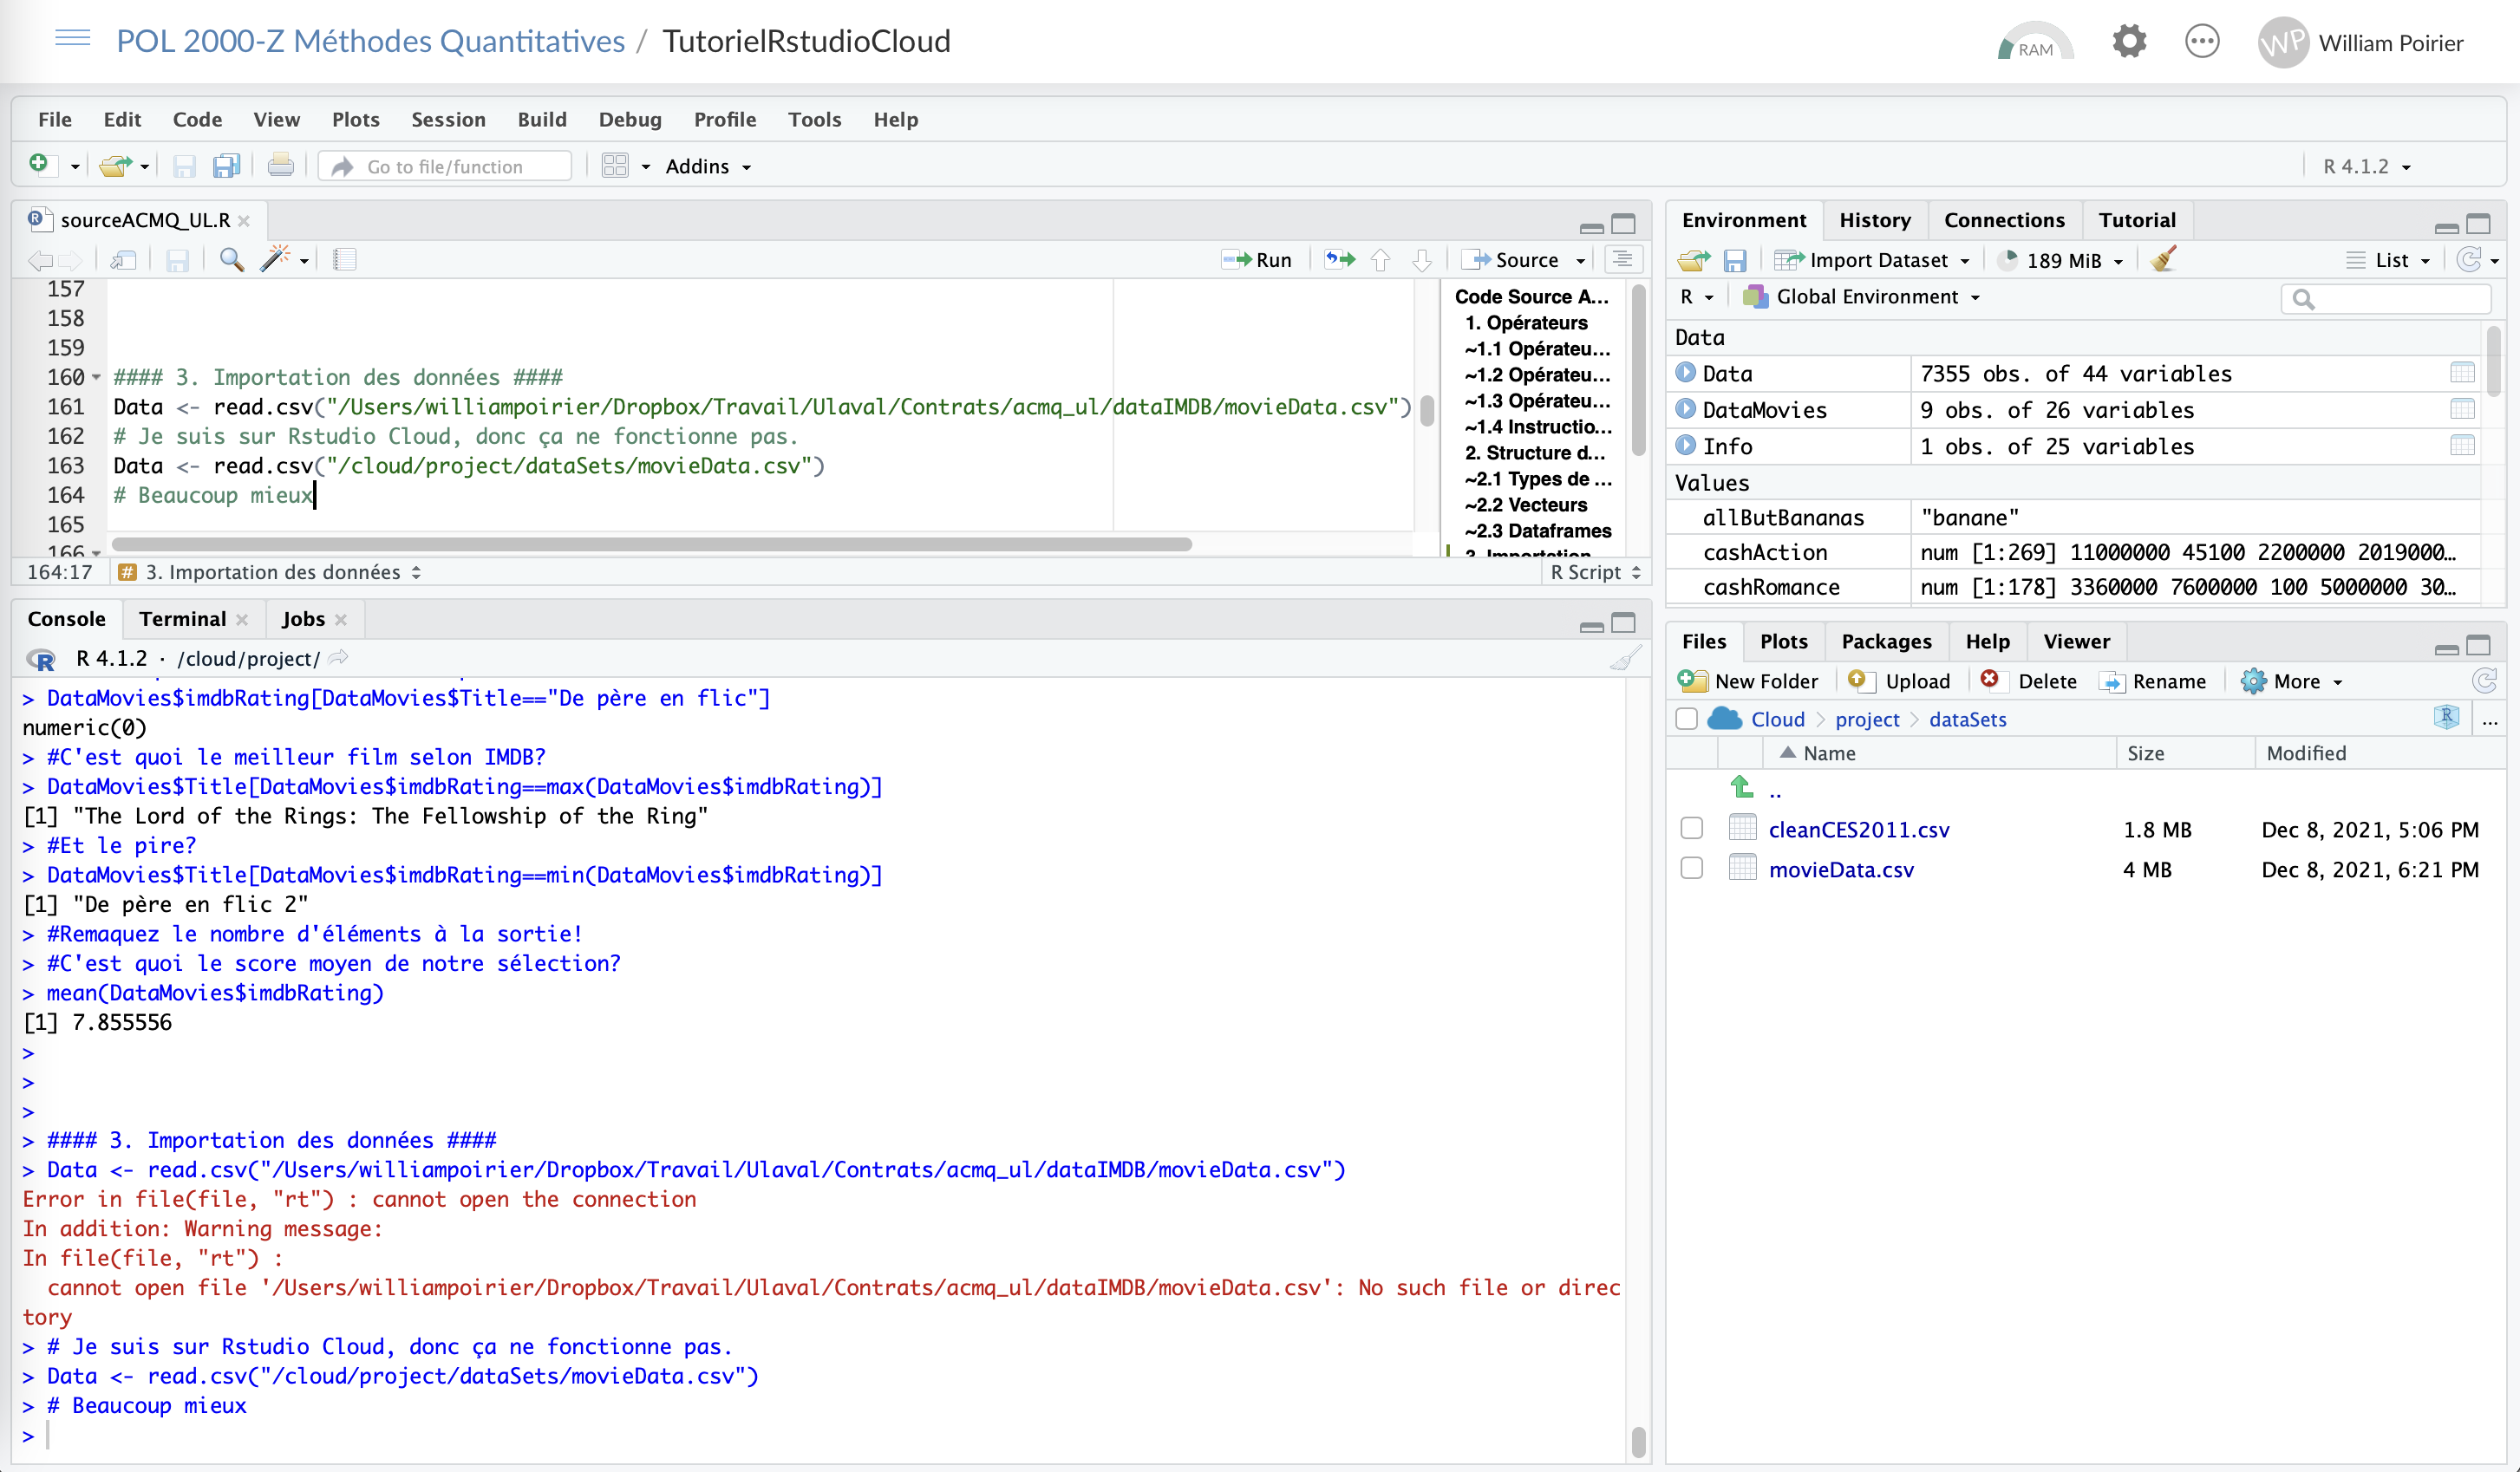
\includegraphics[width=0.98\linewidth]{_graphs/import.png}}
    \caption{Importer des données à un environnement de travail}
    \label{importFig}
    \end{figure}

  
\section{Importation de données}\label{import}
  \subsection{Importation de données}
  Avant de débuter l'analyse, il faut des données à analyser. En science politique, les bases de données auxquelles vous ferez face seront typiquement rectangulaires. Elles auront donc la même structure qu'un \emph{data frame} tel que compris par \textbf{R}: un cas par ligne, une variable par colonne. Si vous êtes familier avec Excel, vous reconnaîtrez certainement cette structure. 
  
  \textbf{R} étant un langage \emph{open source}, la communauté de développement donne accès à plusieurs librairies (\emph{packages}) dédiées à la lecture de différents formats de données. Dans le cadre du cours, vous n'aurez uniquement qu'à traiter des données enregistrées en format \rcode{.csv}, valeurs séparées par des virgules (\emph{comma-separated values}). C'est ce qui se cache derrière les tableaux Excel. Or, les formats \rcode{.sav}, \rcode{.spss}, \rcode{.rds}, et \rcode{.tsv} sont également populaires. Si vous rencontrez un jour l'un de ces formats, il est certain qu'une fonction pour les ouvrir existe déjà. À ce moment, \textbf{Google} sera votre meilleur ami! Une fois la bonne fonction identifiée, la procédure est assez simple si l'on comprend bien le concept d'arborescence. Je vous invite donc à réviser la section \ref{arborescence} avant de continuer. 
  
  Pour ouvrir un fichier \rcode{.csv}, il faut exécuter la fonction \rcode{read.csv()} et assigner le résultat à un objet (typiquement appelé \emph{Data}) comme le montre la figure \ref{importFig}. Il est important de constater que le seul argument requis est l'arborescence menant au fichier \rcode{.csv} que vous voulez ouvrir. Dans le cas de la figure \ref{importFig} à la ligne 161, il s'agit d'une arborescence d'ordinateur Mac typique. Pour un PC, un \rcode{C:} aurait été ajouté devant \rcode{/Users}. La procédure est similaire pour un projet \textbf{RStudio Cloud}. Or, il faut d'abord télécharger le fichier dans le projet \textbf{RStudio Cloud}.
  
  \textbf{RStudio Cloud} est une plateforme web. Ce faisant, elle n'a pas directement accès à votre ordinateur comme c'est le cas si vous utilisez \textbf{RStudio}. Référez-vous à la figure \ref{homeMenu} pour savoir comment créer un projet. Une fois le projet créé, vous pouvez ajouter un fichier de données en appuyant sur le bouton \textit{upload}. Vous n'aurez toutefois pas à le faire normalement. En effet, les projets \textbf{RStudio Cloud} nous permettent de créer un environnement identique pour tous les étudiants et d'y ajouter les fichiers nécessaires. Ainsi, si vous créez votre propre projet à partir de l'espace de travail \emph{POL 2000-Z Méthodes Quantitatives}, vous aurez accès à tout ce dont vous aurez besoin. 

  
\section{Analyse - Description}
L'analyse descriptive des données est l'outil de base du chercheur voulant explorer une base de données. Cette section présentera les principaux tests, visualisations et mesures d'analyse descriptive.
  \subsection{Univariée}
  Une analyse univariée est, comme son nom l'indique, une analyse s'effectuant sur UNE SEULE variable. Vous avez déjà rencontré les principales mesures lui étant associé à la figure \ref{struVec2}. En effet, ce qui nous intéresse dans ce genre d'analyse est la distribution d'une variable. Est-elle distribuée normalement ou est-elle asymétrique? Quel est son mode? Sa variance? Les \textbf{mesures de dispersion} permettent d'identifier le positionnement des observations sur la distribution et de répondre à ces questions. Ainsi, pour obtenir la moyenne d'une variable, il faut utiliser la même fonction qu'à la figure \ref{struVec2} en indiquant cette fois la bonne colonne du \emph{data frame} où se trouve la variable d'intérêt (\rcode{mean(Data\$nomDeLaVariable)}). Rappelez-vous: les colonnes d'un \emph{data frame} ne sont que des vecteurs déguisés!
  
  \subsection{Bivariée}
  Vous vous en doutez certainement, si une analyse univariée se concentre sur une seule variable, une analyse bivariée en compare deux. Étonnant, n'est-ce pas?! Plusieurs tests existent pour comparer deux variables, nous vous en présenterons deux: le test-t de Student et le r de Pearson. 
  
  Le test-t de Student permet d'effectuer un test d'hypothèse statistique. Il est souvent utilisé pour déterminer si les distributions (ou les moyennes) de deux variables sont significativement différentes. Par exemple, si on s'intéresse à la différence de revenu collecté pour différents types de films, nous pouvons tester les moyennes grâce à un test-t. La figure \ref{anaTtest} montre comment utiliser la fonction \rcode{t.test()}. Celle-ci prend comme arguments principaux deux variables. Dans notre cas, un vecteur du revenu des films romantiques et un vecteur du revenu des films d'action. Remarquez comment sont spécifiés les vecteurs d'intérêt. Si nous utilisions uniquement \rcode{Data\$revenue} en x et en y, le test-t ne remarquerait aucune différence puisque c'est la même variable. Il est également possible de spécifier l'intervalle de confiance désiré. N'oubliez pas, si vous souhaitez plus d'informations sur l'utilisation d'une fonction, inscrivez et exécutez \rcode{?maFonction()} dans la console. Une fenêtre d'information s'ouvrira. 
  
  Le r de Pearson est un test de corrélation simple et pratique qui vous permettra de tester la relation entre deux variables. Distinguez bien les deux concepts. Le test-t permet de tester si deux distributions sont différentes. La corrélation permet, elle, de tester s'il y a une relation entre deux distributions. Attention: une corrélation entre deux variables ne veut pas dire qu'il y a causation! La fonction \textbf{R} pour ce test est utilisée de la même manière que pour le test-t. Il suffit d'identifier les arguments x et y (les deux variables) de la fonction \rcode{cor.test()} comme le montre la figure \ref{anaPearCorr} et le tour est joué.
  
  \begin{figure}[H]
    \centering
    \fbox{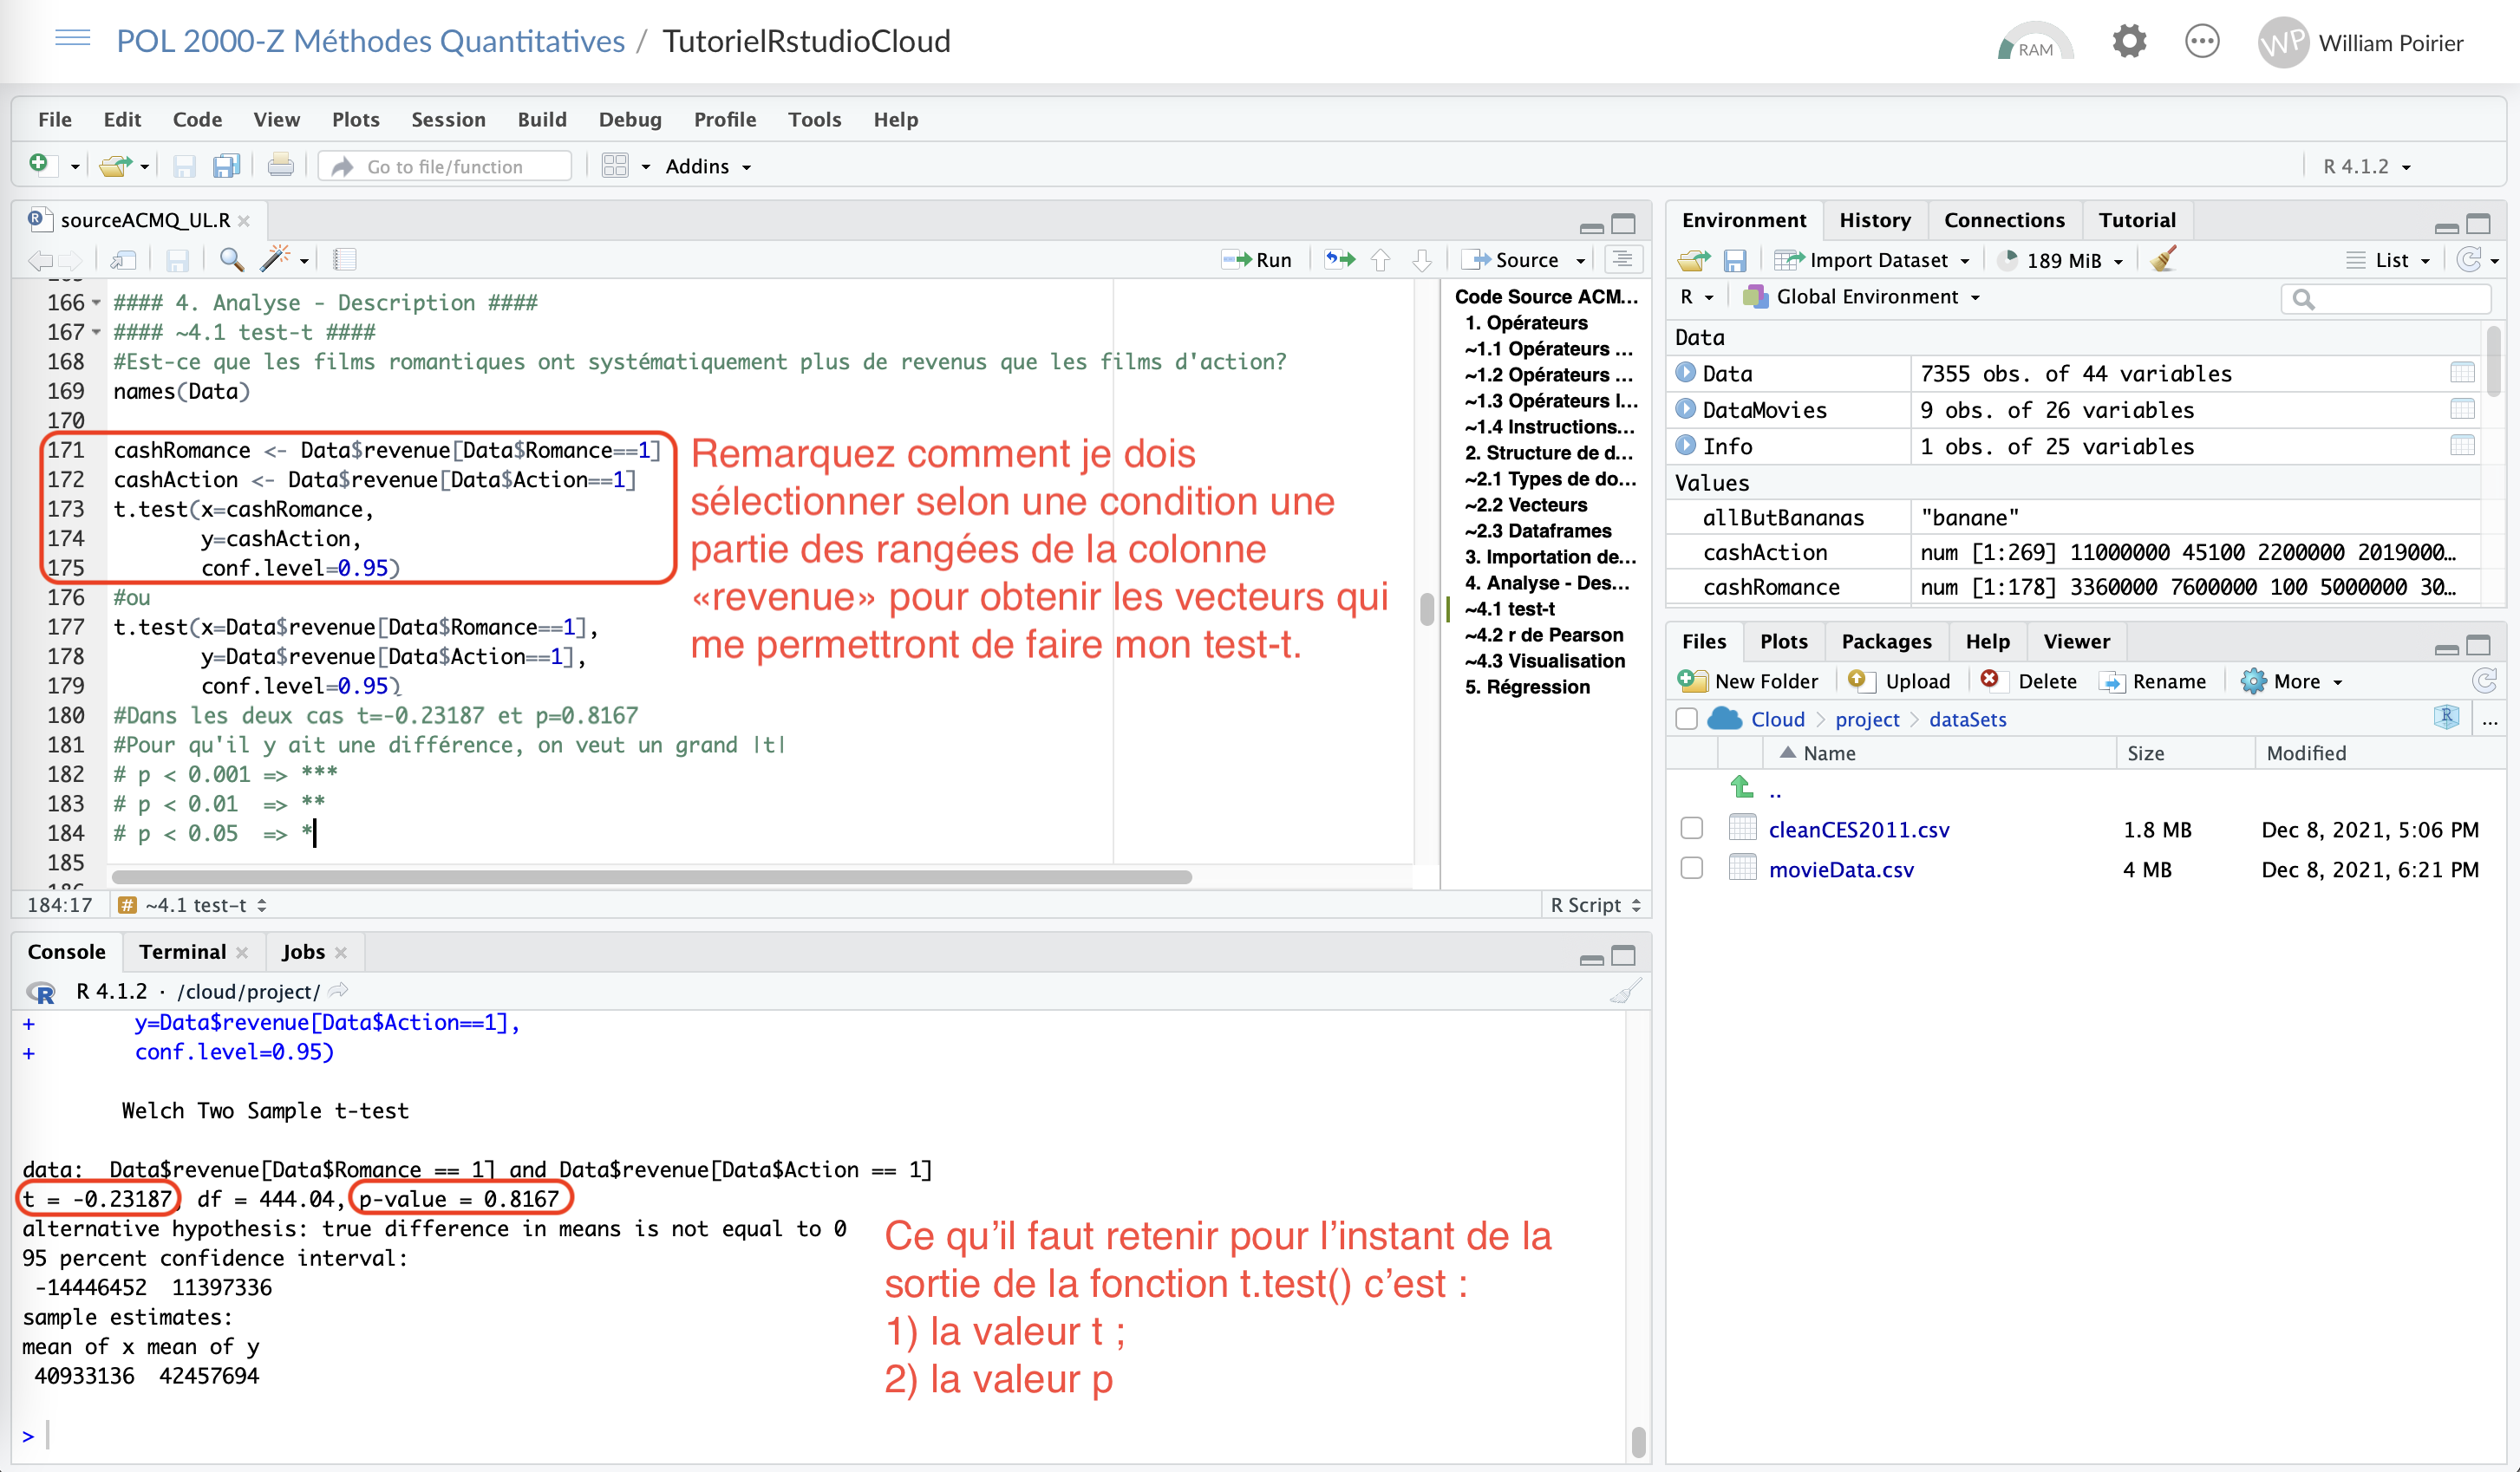
\includegraphics[width=0.98\linewidth]{_graphs/anaTtest.png}}
    \caption{Test t de Student}
    \label{anaTtest}
    \end{figure}
    
    \begin{figure}[H]
    \centering
    \fbox{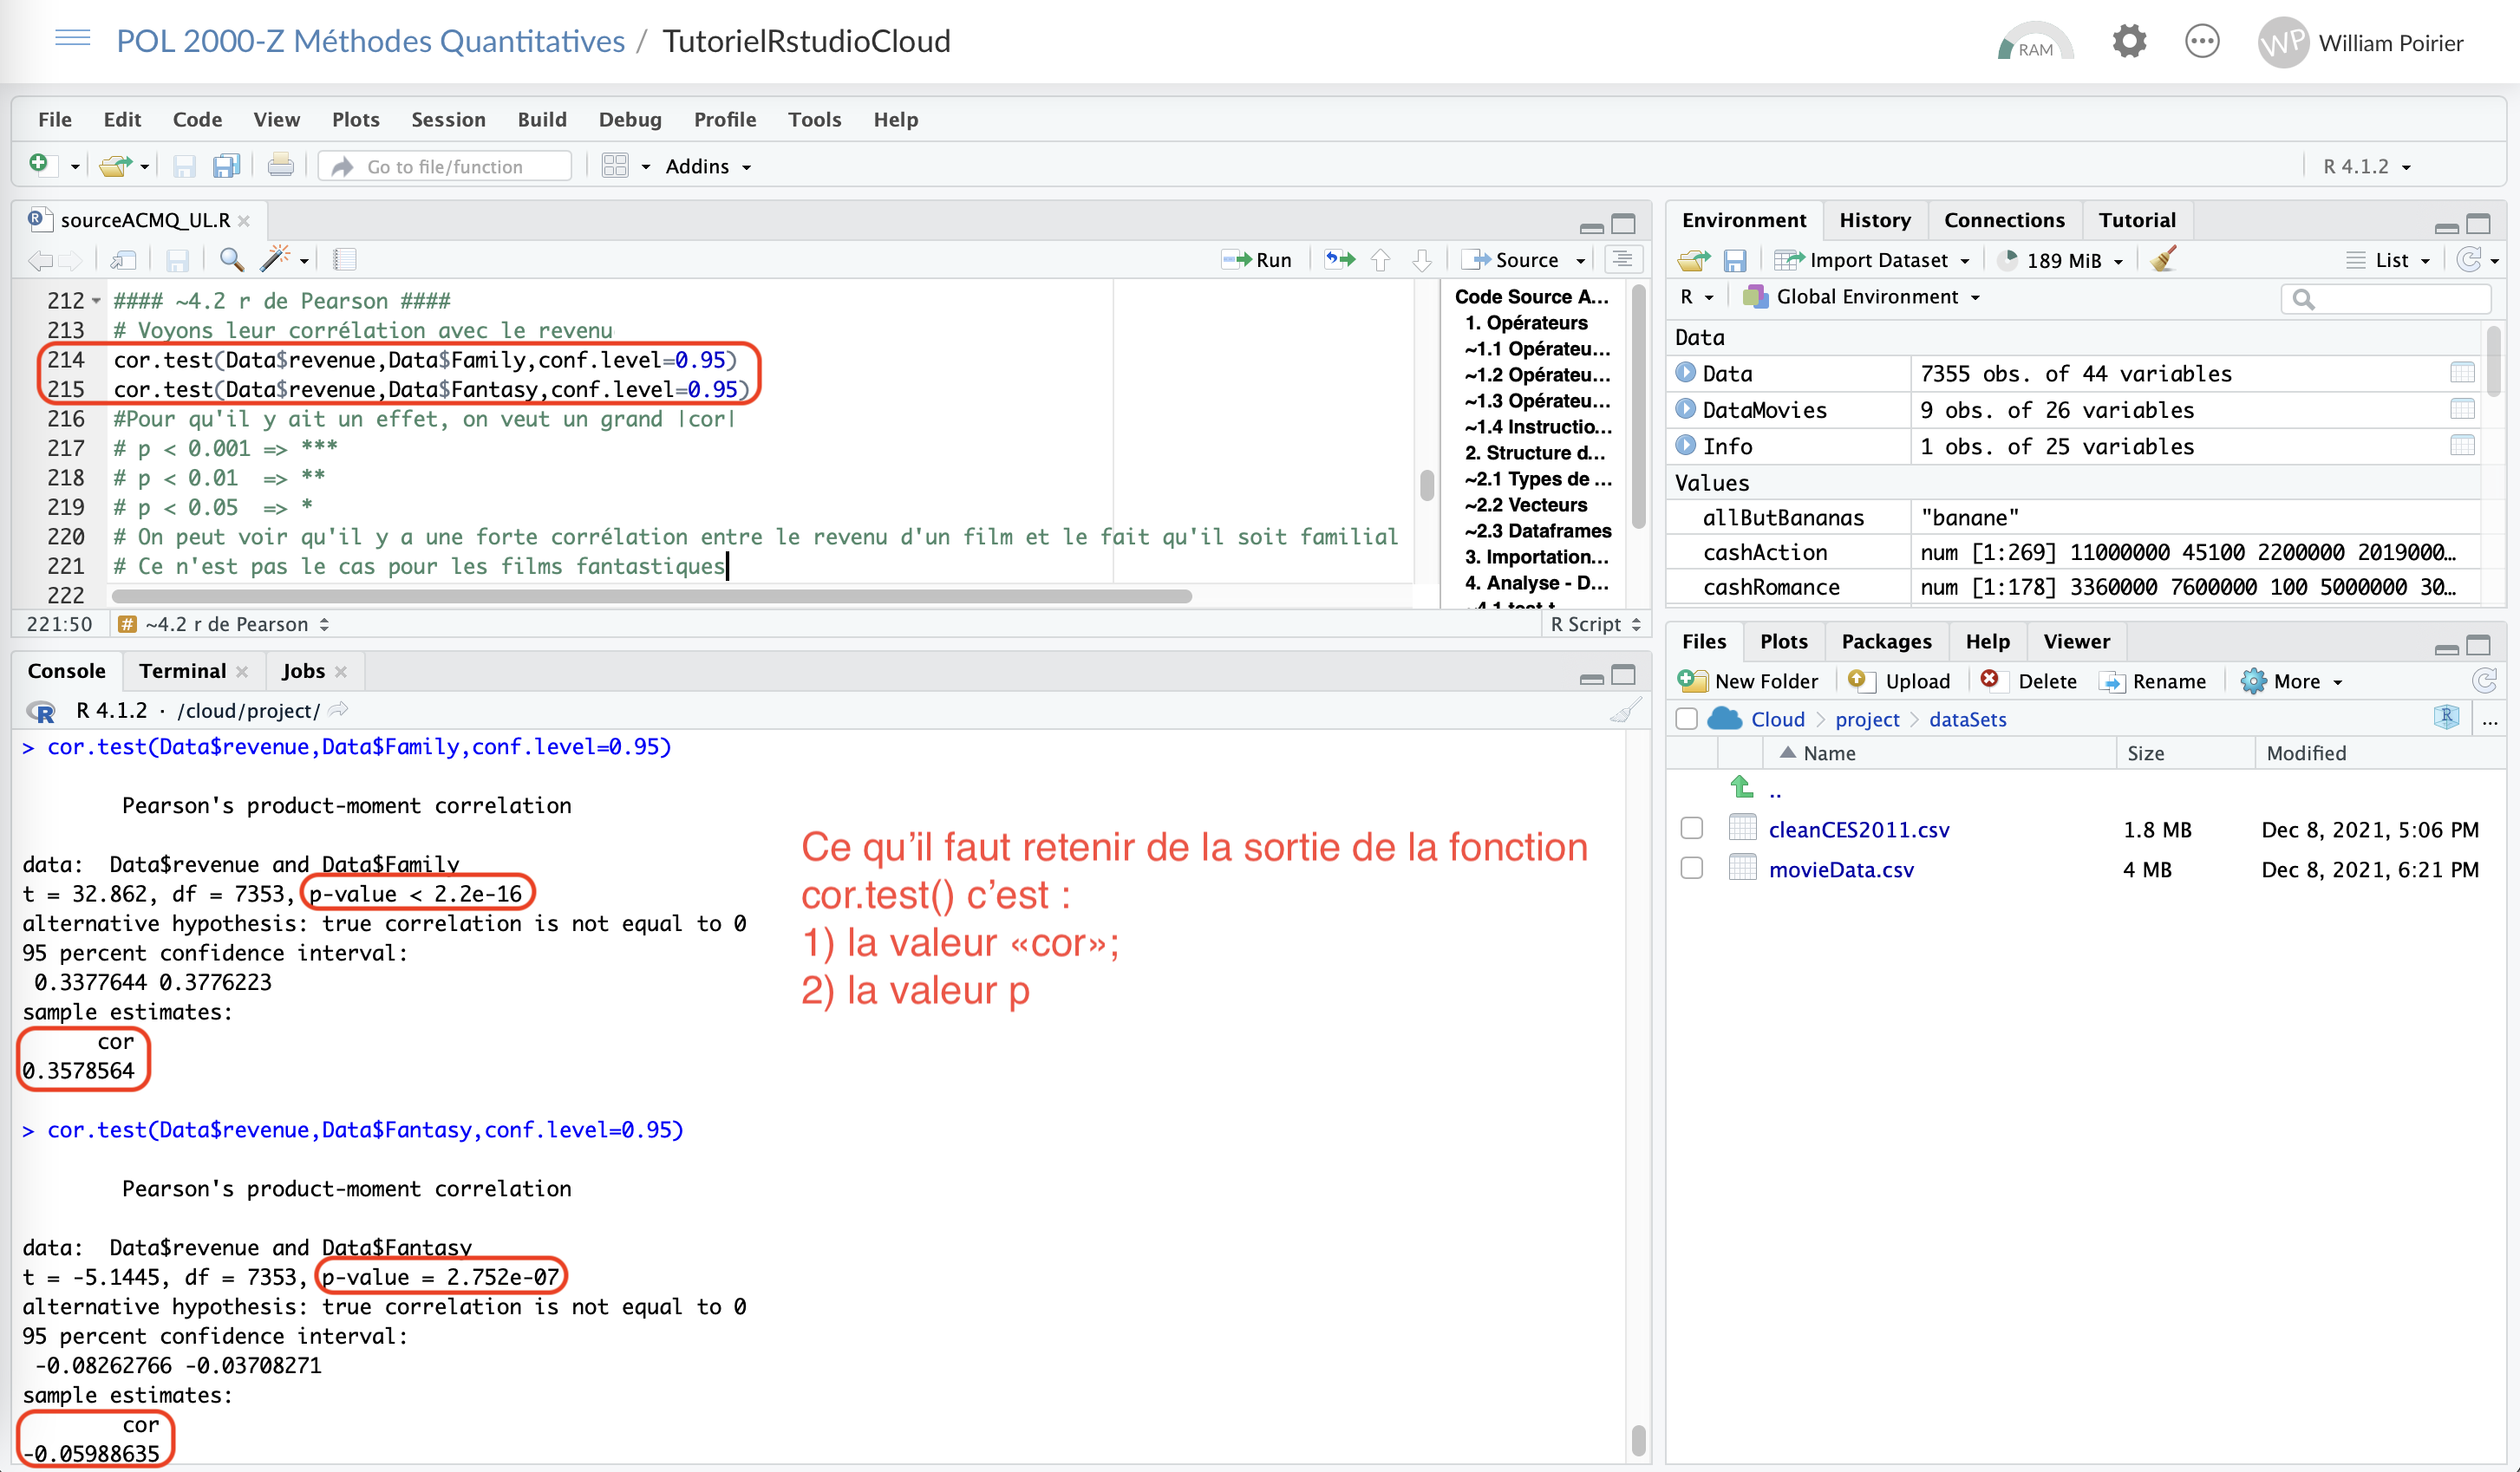
\includegraphics[width=0.98\linewidth]{_graphs/anaPearCorr.png}}
    \caption{Test de corrélation (r de Pearson)}
    \label{anaPearCorr}
    \end{figure}
  
   \begin{figure}[H]
    \centering
    \fbox{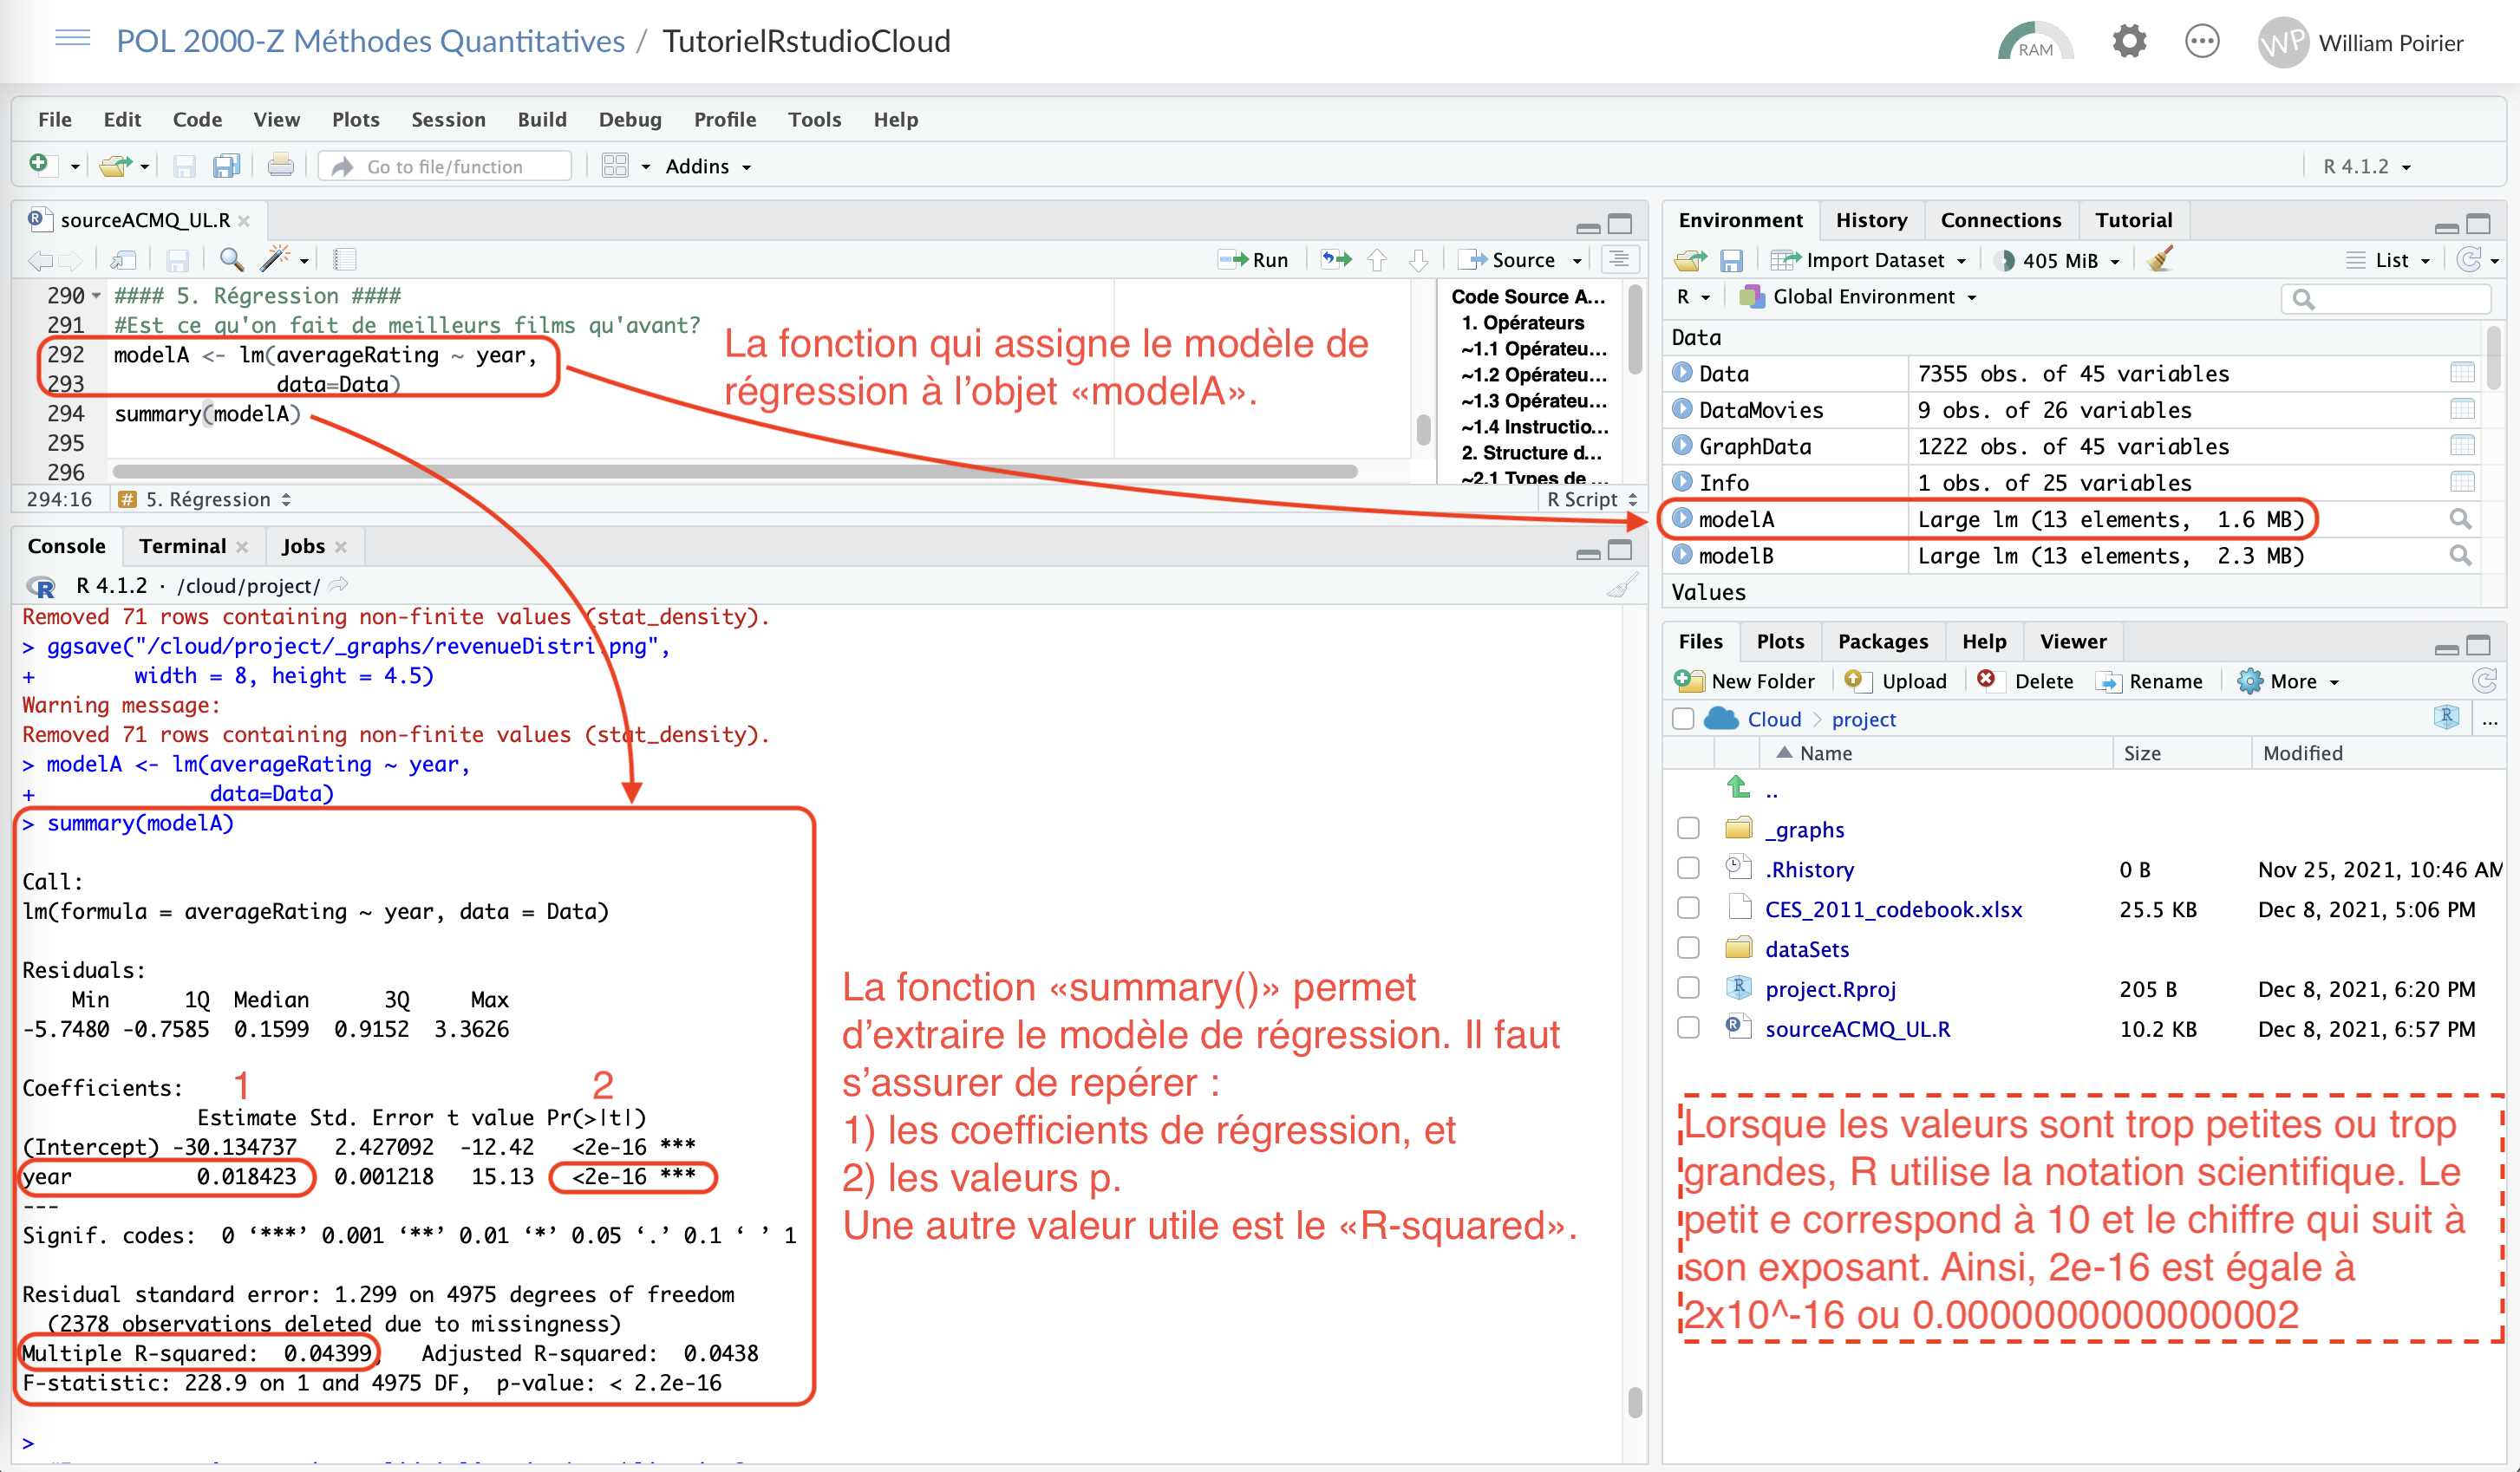
\includegraphics[width=0.98\linewidth]{_graphs/anaReg1.png}}
    \caption{Régression linéaire simple}
    \label{anaReg1}
    \end{figure}
    
      \begin{figure}[H]
    \centering
    \fbox{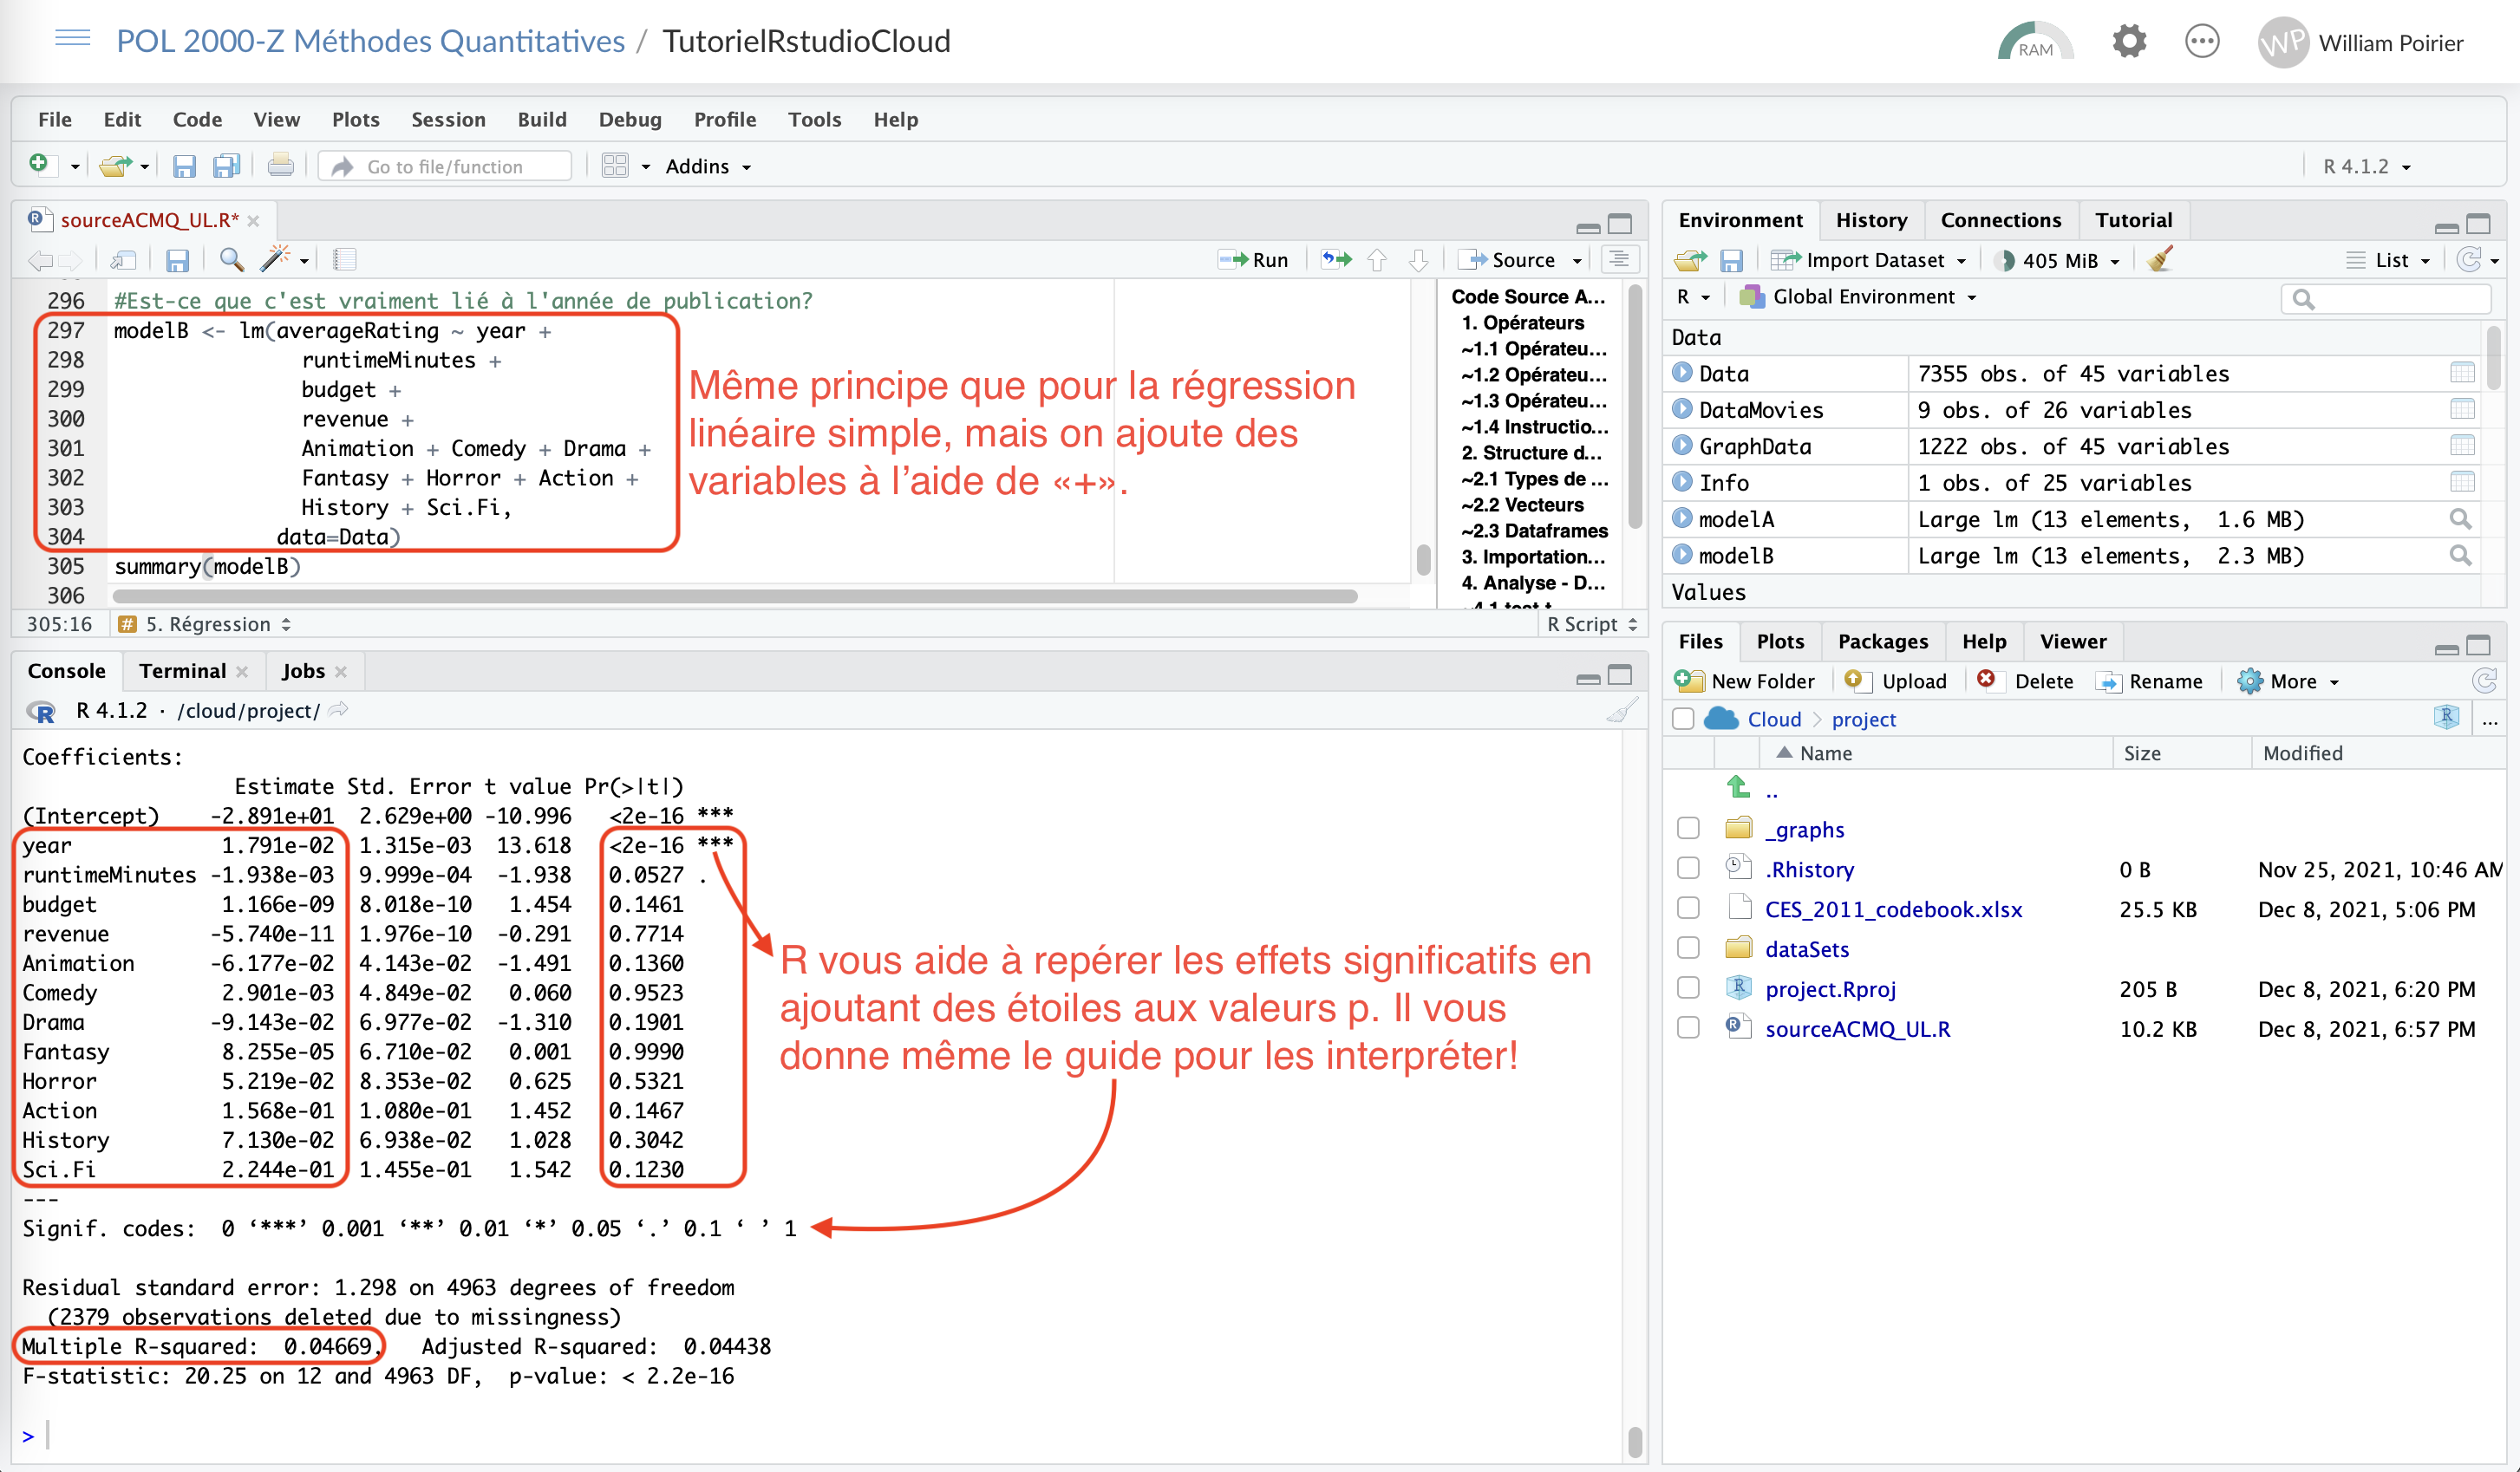
\includegraphics[width=0.98\linewidth]{_graphs/anaReg2.png}}
    \caption{Régression linéaire multiple}
    \label{anaReg2}
    \end{figure}

  
  \section{Analyse - Régression linéaire simple et multiple}
  La régression est sans doute l'outil le plus utile de l'arsenal de l'analyse quantitative. Elle est à la base de plusieurs modèles statistiques plus avancés allant même jusqu'à l'apprentissage machine. Le principe de la régression devrait vous être plus familier à la suite du cours. Cette section se concentrera donc sur la façon d'en faire avec \textbf{R}.

  La fonction \rcode{lm()} permet de calculer un modèle de régression comme le montre la figure \ref{anaReg1}. Le premier argument est toujours la variable dépendante (ou variable prédite) suivie d'un tilda ($\sim$) et de la ou des variables indépendantes. Celles-ci s'ajoutent à l'aide du \rcode{+}. Une fois toutes les variables du modèle spécifiées, il faut ajouter une virgule suivie de l'argument \rcode{data=} et du bon \textit{data frame}. Attention, il est important d'utiliser le même nom de variable que les noms associés aux colonnes du \textit{data frame} en question. À la figure \ref{anaReg1}, on assigne l'extrant de la fonction à un objet appelé \rcode{modelA}. De cette façon, il est possible d'utiliser la fonction \rcode{summary(modelA)} pour obtenir plus d'informations sur le modèle. La figure \ref{anaReg2} présente un modèle de régression multiple. La différence? Il y a plus de variables après les \rcode{+}. Voilà! Vous savez coder un modèle de régression linéaire en \textbf{R} maintenant. C'est aussi simple que ça!  
  
  \section{Visualisation}
  Bien souvent, il est difficile de se souvenir de l'interprétation des différents tests et les chiffres sont rarement le meilleur moyen de transmettre l'information à un plus large public. Grâce à \textbf{R} et la fonction \rcode{ggplot()}, il est facile de présenter visuellement les résultats de nos analyses.\footnote{En fait, \rcode{ggplot()} est une fonction issue de la librairie \textit{ggplot2}, elle même issue de la meta-librarie \textit{tidyverse}.} Nous ne ferons ici qu'une introduction aux principales fonctionnalités de \textit{ggplot2}. Pour une revue exhaustive des fonctionnalités, consultez ce \href{https://ggplot2.tidyverse.org/reference/}{lien}.\footnote{Le voici si vous lisez sur papier \href{https://ggplot2.tidyverse.org/reference/}{https://ggplot2.tidyverse.org/reference/}}
  
  \rcode{ggplot} s'attend à recevoir au moins 3 éléments présentés aux lignes 225-26 de la figure \ref{visGeom} : 1) un \emph{data frame}, 2) un \textit{aesthetic}, et 3) un \rcode{geom}. Le \emph{data frame} contient les informations qui composeront le graphique. Il peut s'agir de la base de données originale, d'un sous-échantillon ou même des résultats d'une analyse quelconque (une suite de moyennes par année, par exemple). L'\textit{aesthetic} (ou \rcode{aes}) contient les arguments permettant d'identifier le rôle des variables d'intérêt du \emph{data frame}. C'est là où sont spécifiés l'axe des X, l'axe des Y, et la façon d'associer les groupes par couleur ou par texture. Par exemple, aux lignes 225-26 de la figure \ref{visGeom}, il est seulement spécifié que la variable \rcode{runtimeMinutes} correspond à l'axe des X. Pourquoi n'est-il pas spécifié un axe des Y ? C'est là qu'entrent en jeu les \rcode{geom}. Ce sont essentiellement les fonctions qui vous permettent de spécifier ce qui doit être dessiné. Voici une liste des principaux \rcode{geom} :
  
  \begin{itemize}
    \item \rcode{geom\_histogram()} $\mapsto$ un histogramme
    \item \rcode{geom\_bar()} $\mapsto$ un graphique à barres
    \item \rcode{geom\_col()} $\mapsto$ un graphique à barres\footnote{La différence entre \rcode{geom\_bar()} et \rcode{geom\_col()} est que \rcode{geom\_bar()} prend une fonction en Y (\rcode{..count..} par exemple) alors que \rcode{geom\_col()} prend une variable.}
    \item \rcode{geom\_point()} $\mapsto$ un nuage de points
    \item \rcode{geom\_smooth()} $\mapsto$ une courbe de régression
  \end{itemize}
  
%  \begin{itemize}
%    \item \rcode{geom\_histogram()} $\mapsto$ un histogramme
%    \item \rcode{geom\_bar()} $\mapsto$ un graphique à barres
%    \item \rcode{geom\_col()} $\mapsto$ un graphique à barres\footnote{La différence entre \rcode{geom\_bar()} et \rcode{geom\_col()} est %que \rcode{geom\_bar()} prend une fonction en Y (\rcode{..count..} par exemple) alors que \rcode{geom\_col()} prend une variable.}
%    \item \rcode{geom\_boxplot()} $\mapsto$ un graphique boîte à moustaches 
%    \item \rcode{geom\_density()} $\mapsto$ un tracé de densité
%    \item \rcode{geom\_violin()} $\mapsto$ un graphique en violon
%    \item \rcode{geom\_point()} $\mapsto$ un nuage de points
%    \item \rcode{geom\_jitter()} $\mapsto$ un nuage de points avec bruit
%    \item \rcode{geom\_line()} $\mapsto$ un graphique à lignes
%    \item \rcode{geom\_hline()} $\mapsto$ une ligne horizontale
%    \item \rcode{geom\_vline()} $\mapsto$ une ligne verticale
%    \item \rcode{geom\_smooth()} $\mapsto$ une courbe de régression
%    \item \rcode{geom\_errorbar()} $\mapsto$ des barres d'erreurs
%  \end{itemize}

  Ce qu'il faut bien comprendre, c'est que les arguments de l'\textit{aesthetic} doivent bien s'agencer avec le \rcode{geom} voulu. Par exemple, un histogramme n'a pas besoin d'une position en Y puisque le \rcode{geom} calcule la fréquence lui-même. Or, pour un nuage de points, il faut spécifier à quelle variable correspond l'axe des X et l'axe des Y. Ainsi, le \emph{data frame}, l'\textit{aesthetic} et le \rcode{geom} doivent être en harmonie pour que la fonction retourne le graphique désiré. Pour vous faciliter la vie, je vous propose de toujours répondre à ces 3 questions avant de tenter la production d'un graphique : 
  \begin{enumerate}
  \item Comment vous imaginez-vous le graphique ? 
  \item Quelles sont les variables d'intérêt ?
  \item Est-ce que mon \emph{data frame} a le bon format ?
  \end{enumerate}
  De cette façon, vous vous assurerez de ne pas faire d'erreurs de logique lors de l'écriture de la fonction. Bien entendu, ces trois questions et les \rcode{geom} ne vous permettent d'accéder qu'à une partie de l'ensemble des possibilités et des fonctionnalités qu'offre \rcode{ggplot}. Que ce soit les couleurs, la taille des points ou des barres, l'espacement des barres, le nom des axes, leur gradation, l'ajout d'un titre, d'un sous-titre, d'une note en bas de page, d'annoter le graphique, d'ajuster la légende, la taille et l'angle du texte, de modifier la grille, la couleur de fond, etc. Tout ceci s'apprend sur le tas à l'aide de Google. Si vous avez une question sur une idée de graphique, forte chance que quelqu'un se soit déjà posé cette question. Demandez à Google!
  
  Le dernier concept à bien comprendre pour utiliser \rcode{ggplot()} à son plein potentiel est le concept de couche. C'est ce qui rend \rcode{ggplot()} aussi versatile. Vous avez sans doute remarqué les petits \rcode{+} à la fin de chaque ligne à la figure \ref{visGeom}. Ceux-ci se traduisent pour \textbf{R} comme «ajoute ce qui suit au-dessus de ce qui se trouve avant». Il est donc possible de superposer les \rcode{geom} afin de présenter plus d'informations aux lecteurs ou de mettre en relief certaines informations. Par exemple, à la figure \ref{visLayers}, un \rcode{geom\_smooth()} est ajouté par-dessus un \rcode{geom\_point()} et un \rcode{geom\_line()} afin de présenter l'augmentation du nombre de films produits au fil des années. La figure \ref{visCode} quant à elle présente le code du graphique de la figure \ref{revenueDistri}. Vous y trouverez un code de visualisation plus avancé qui cartographie les fonctions principales de modification de l'aspect visuel du graphique. Il est fortement recommandé d'exécuter le code ligne par ligne afin d'identifier ce que fait chaque partie de la fonction. Comme pour toute chose, c'est en pratiquant que vous apprendrez! 
  
  La fonction \rcode{ggsave()} permet d'enregistrer sous différents formats (pdf, png, jpeg, gif, mp4, etc.) les graphiques produits à l'aide de \rcode{ggplot()}. Pour ce faire, il faut spécifier l'arborescence en la terminant par le nom du fichier suivi de l'extension (.png) désirée. Le ratio largeur:hauteur (\textit{width:height}) peut être spécifié ou non. Dans le cas de la figure \ref{revenueDistri}, le ratio spécifié permet de respecter le standard des images Twitter de 16:9. 
  
  \begin{figure}[H]
    \centering
    \fbox{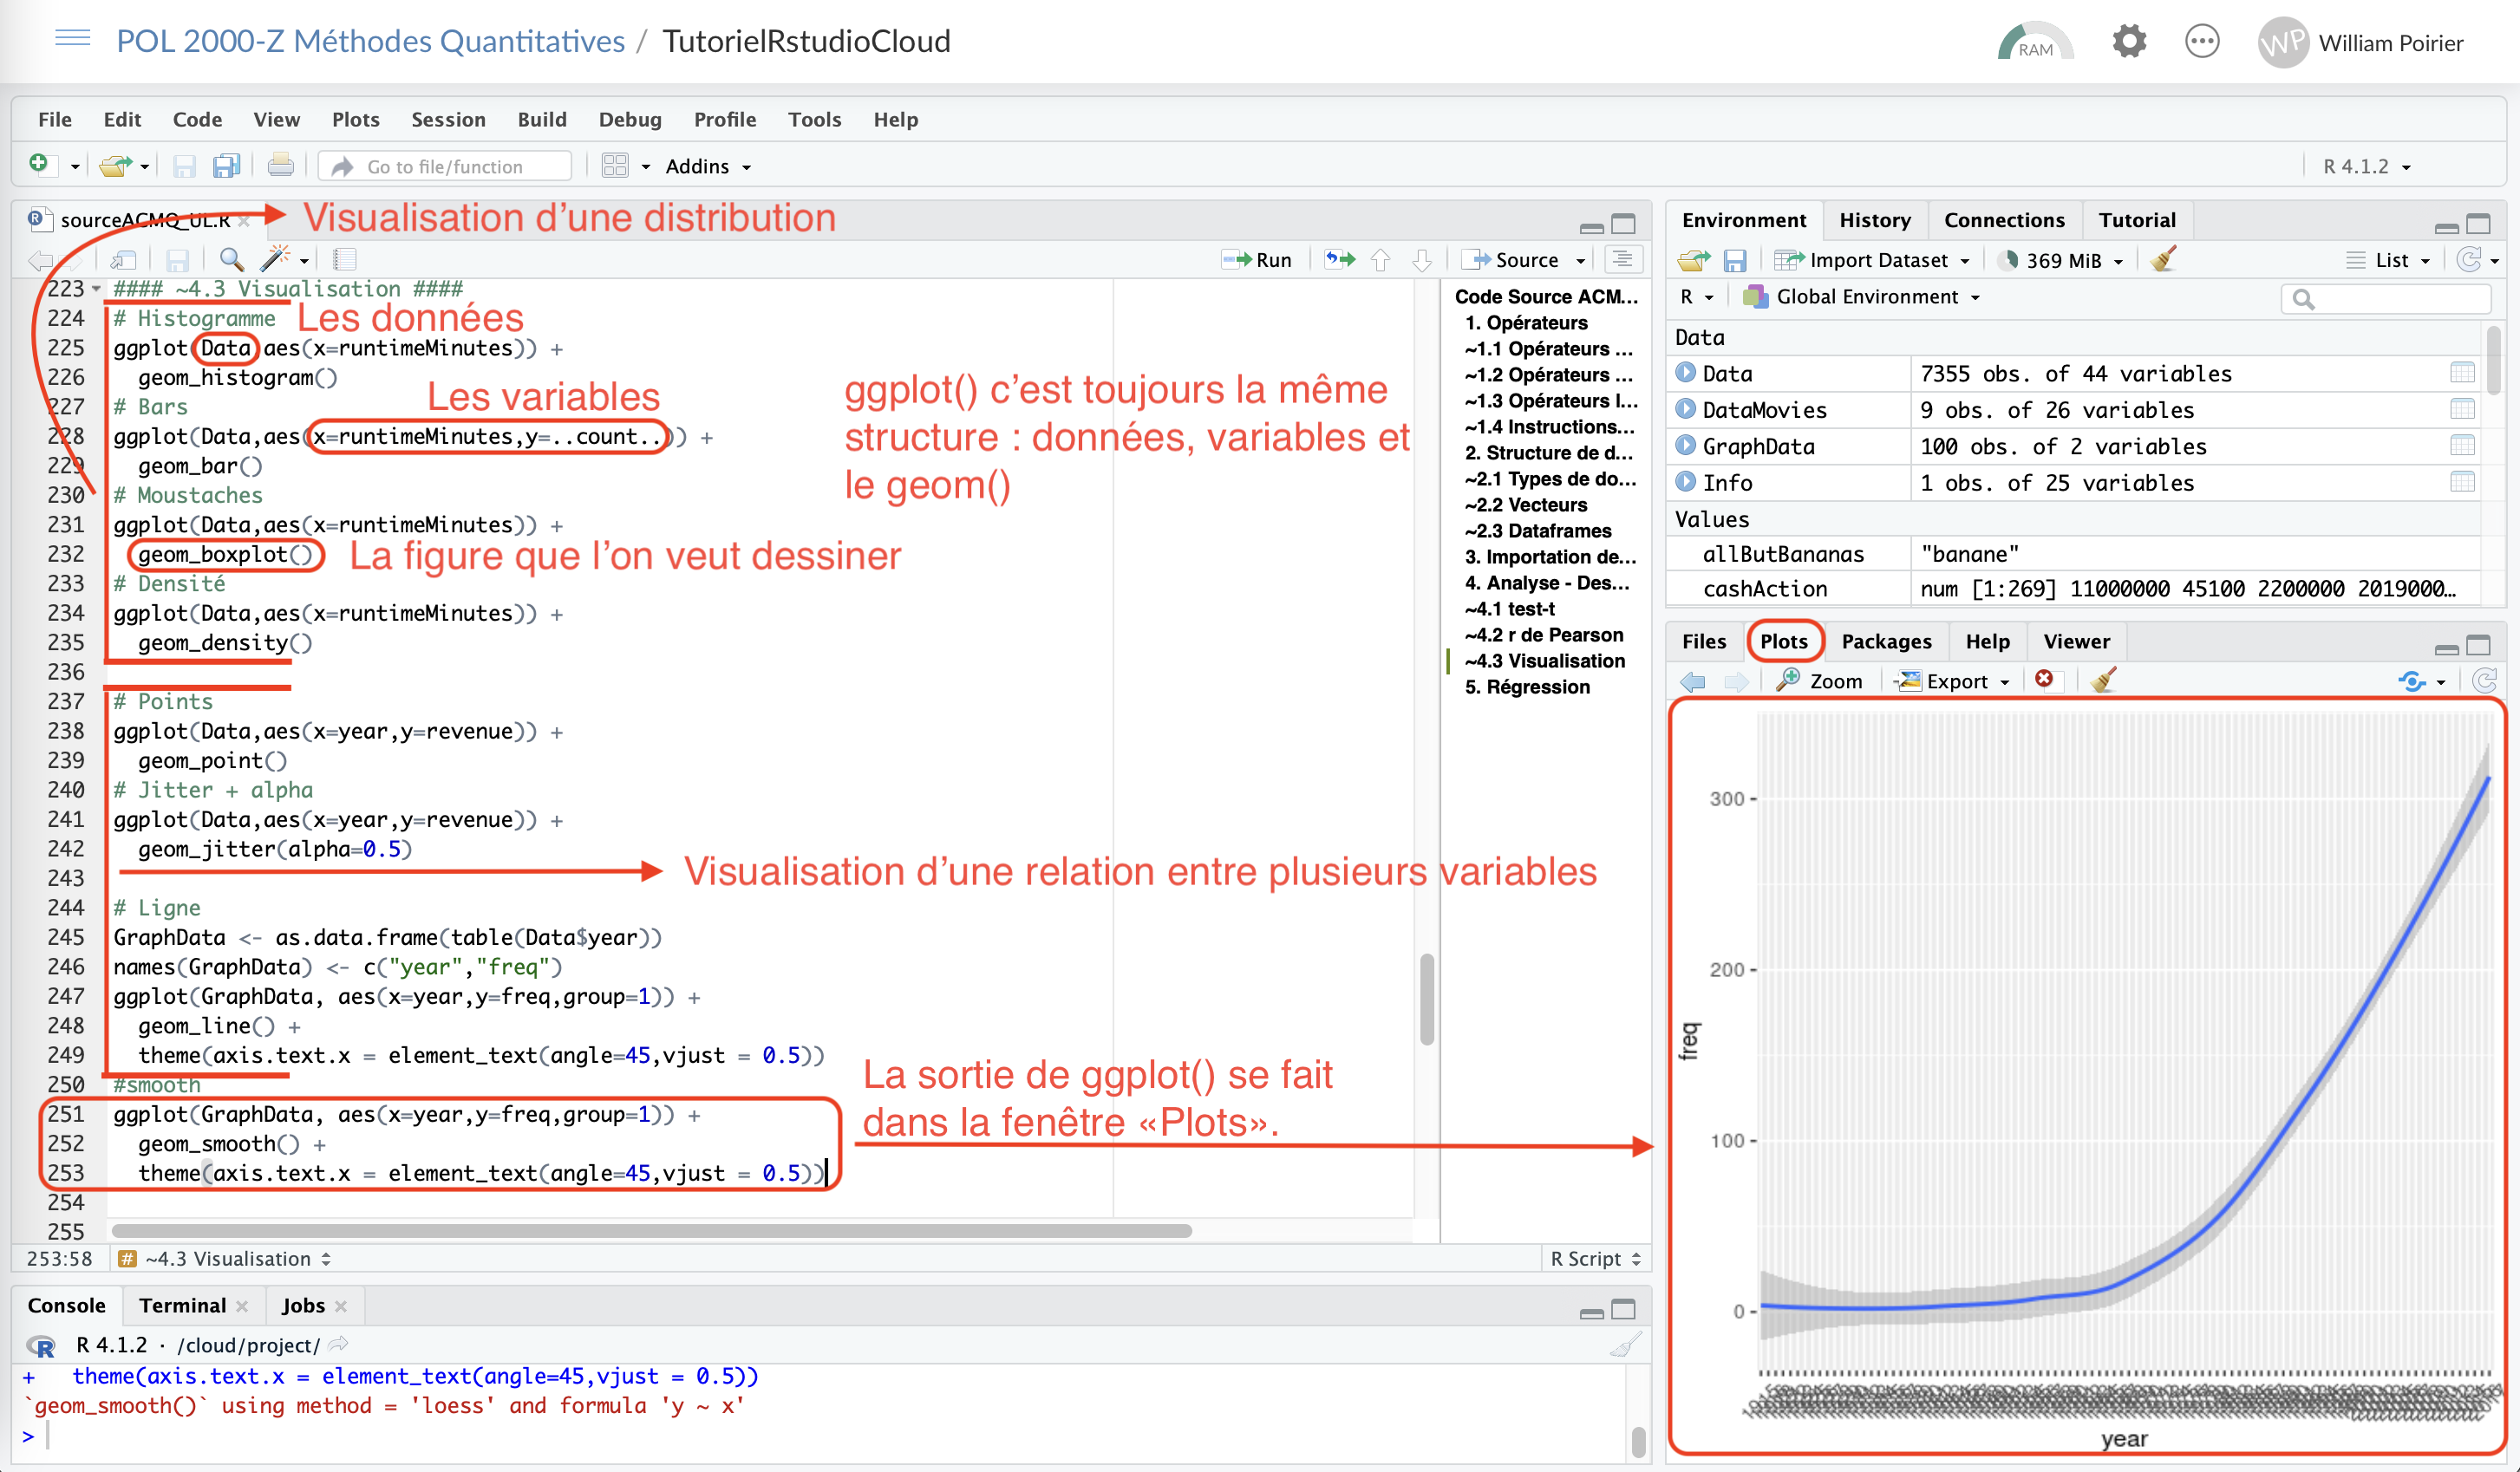
\includegraphics[width=0.98\linewidth]{_graphs/visGeom.png}}
    \caption{Quelques exemples d'utilisation de \rcode{ggplot2}}
    \label{visGeom}
    \end{figure}
  
  \begin{figure}[H]
    \centering
    \fbox{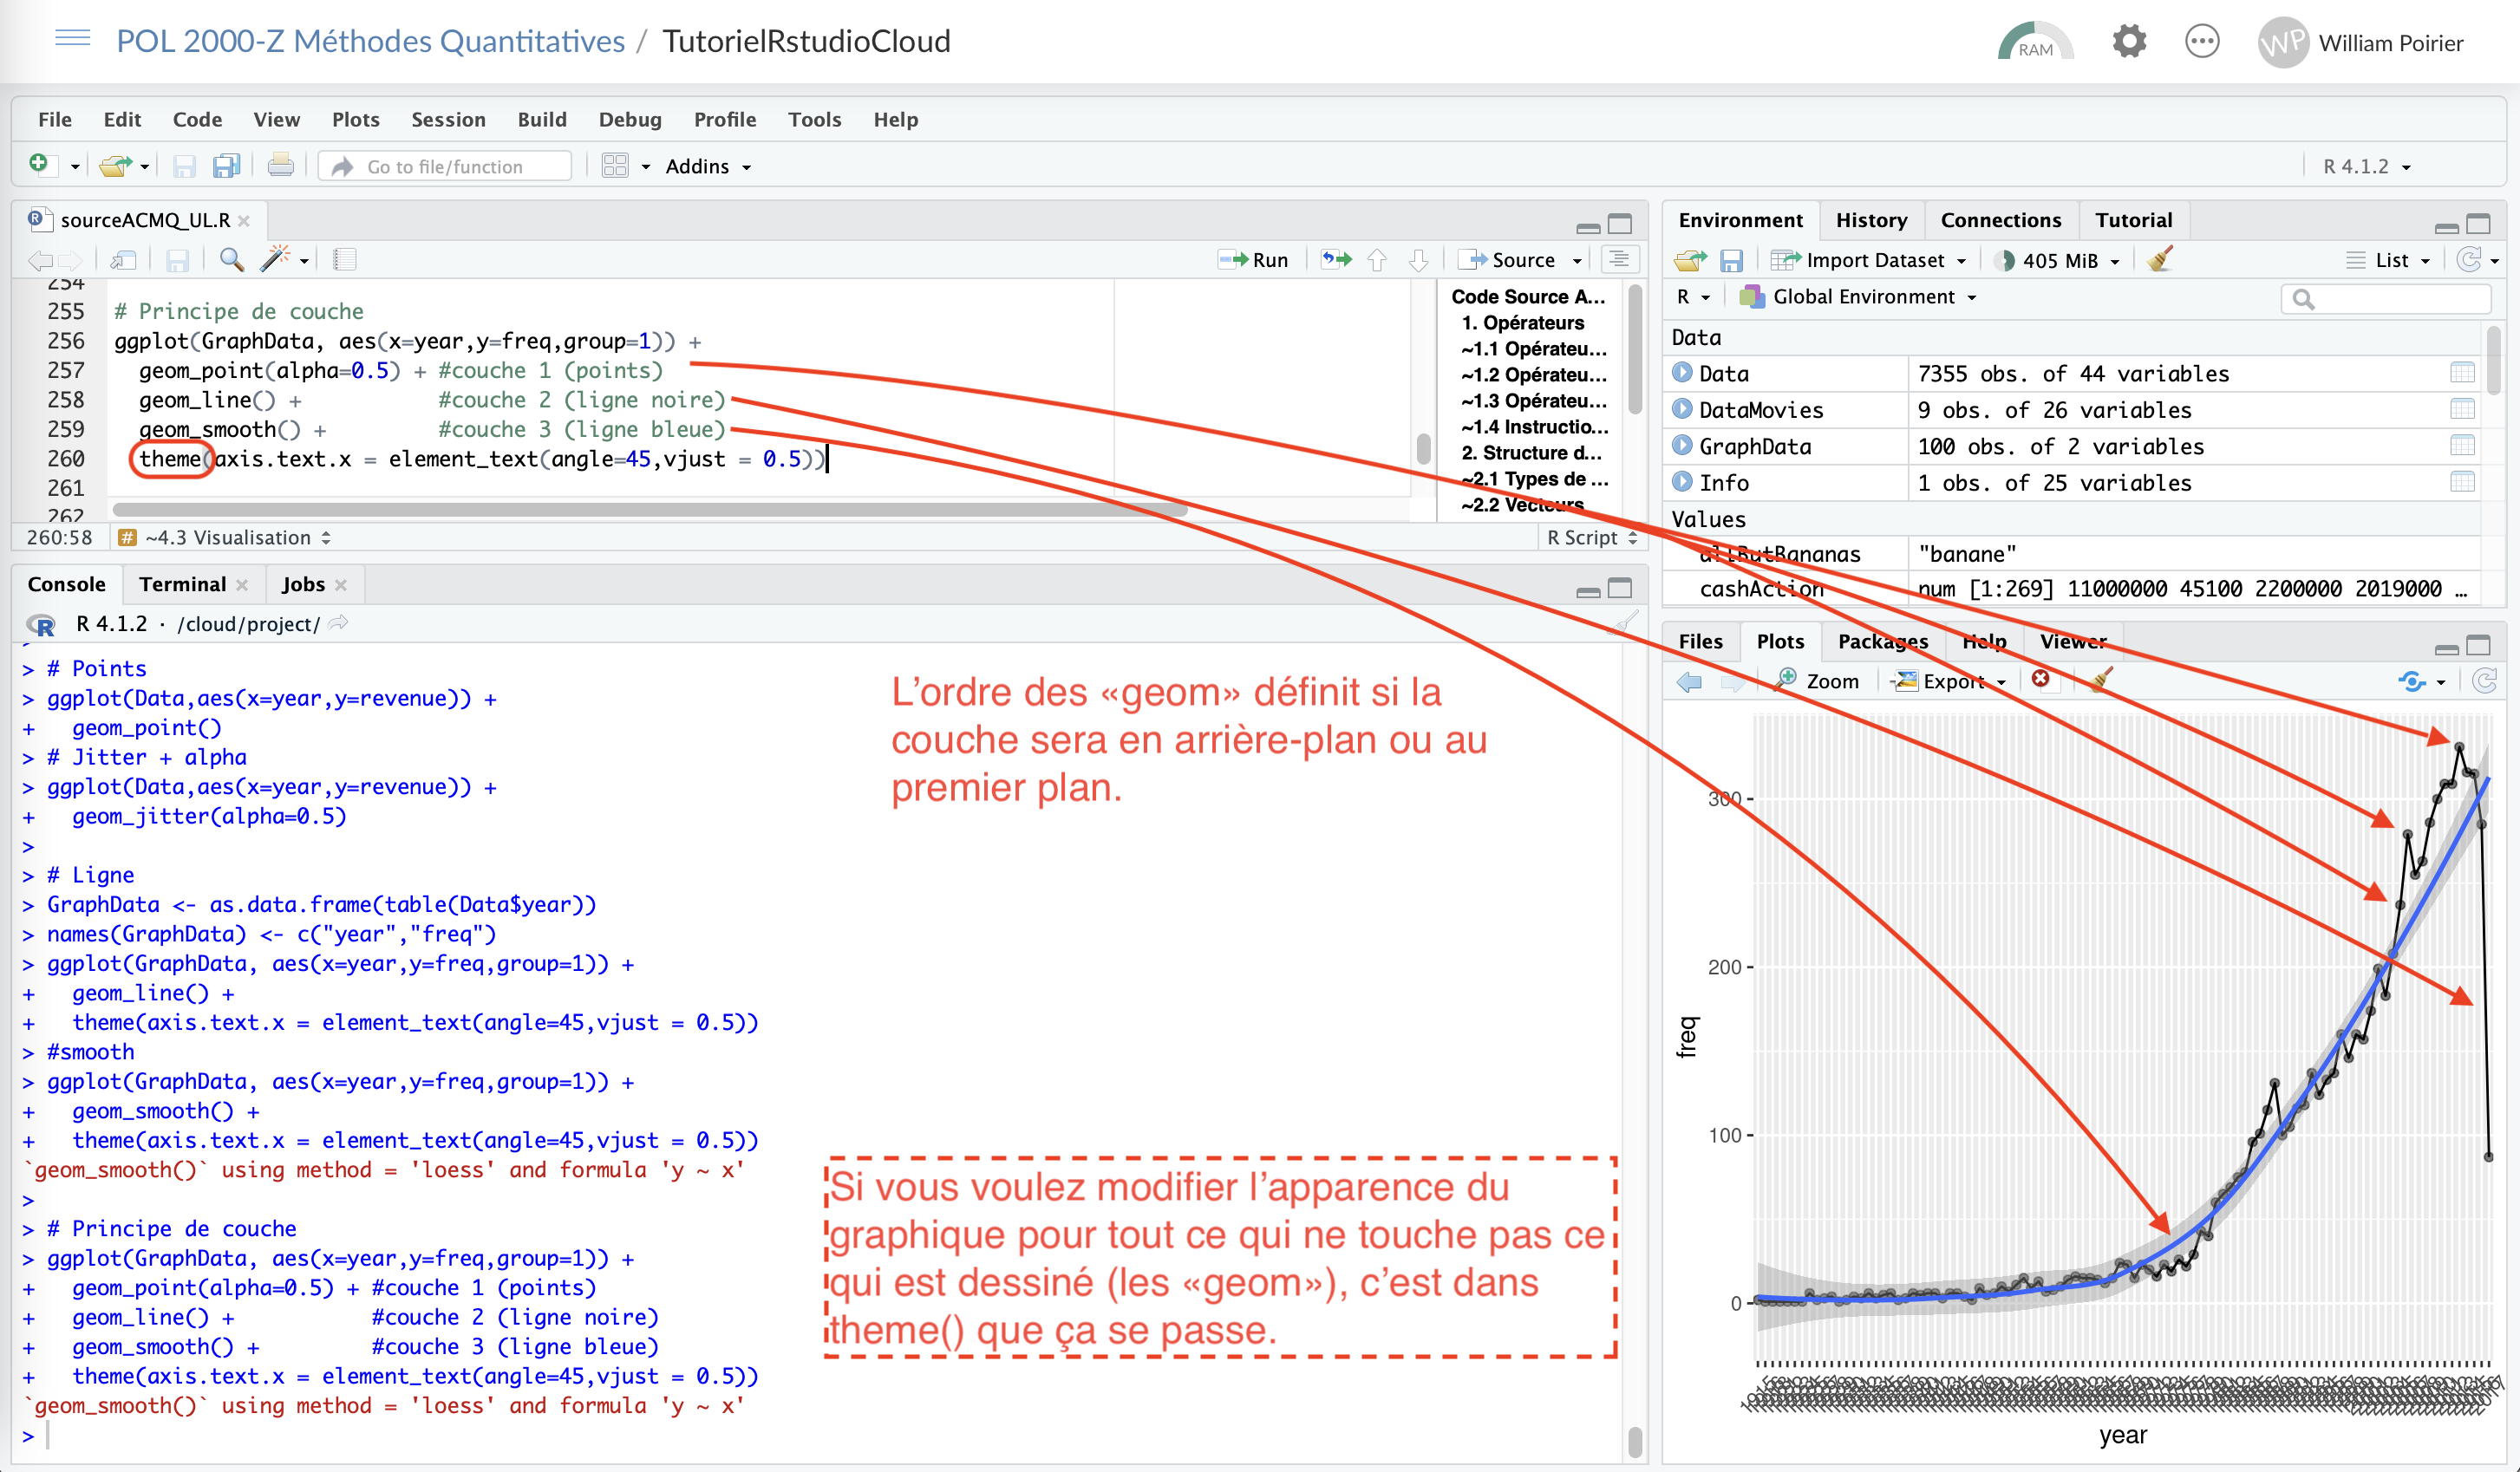
\includegraphics[width=0.98\linewidth]{_graphs/visLayers.png}}
    \caption{Illustration du principe de couche}
    \label{visLayers}
    \end{figure}
    
    \begin{figure}[H]
    \centering
    \fbox{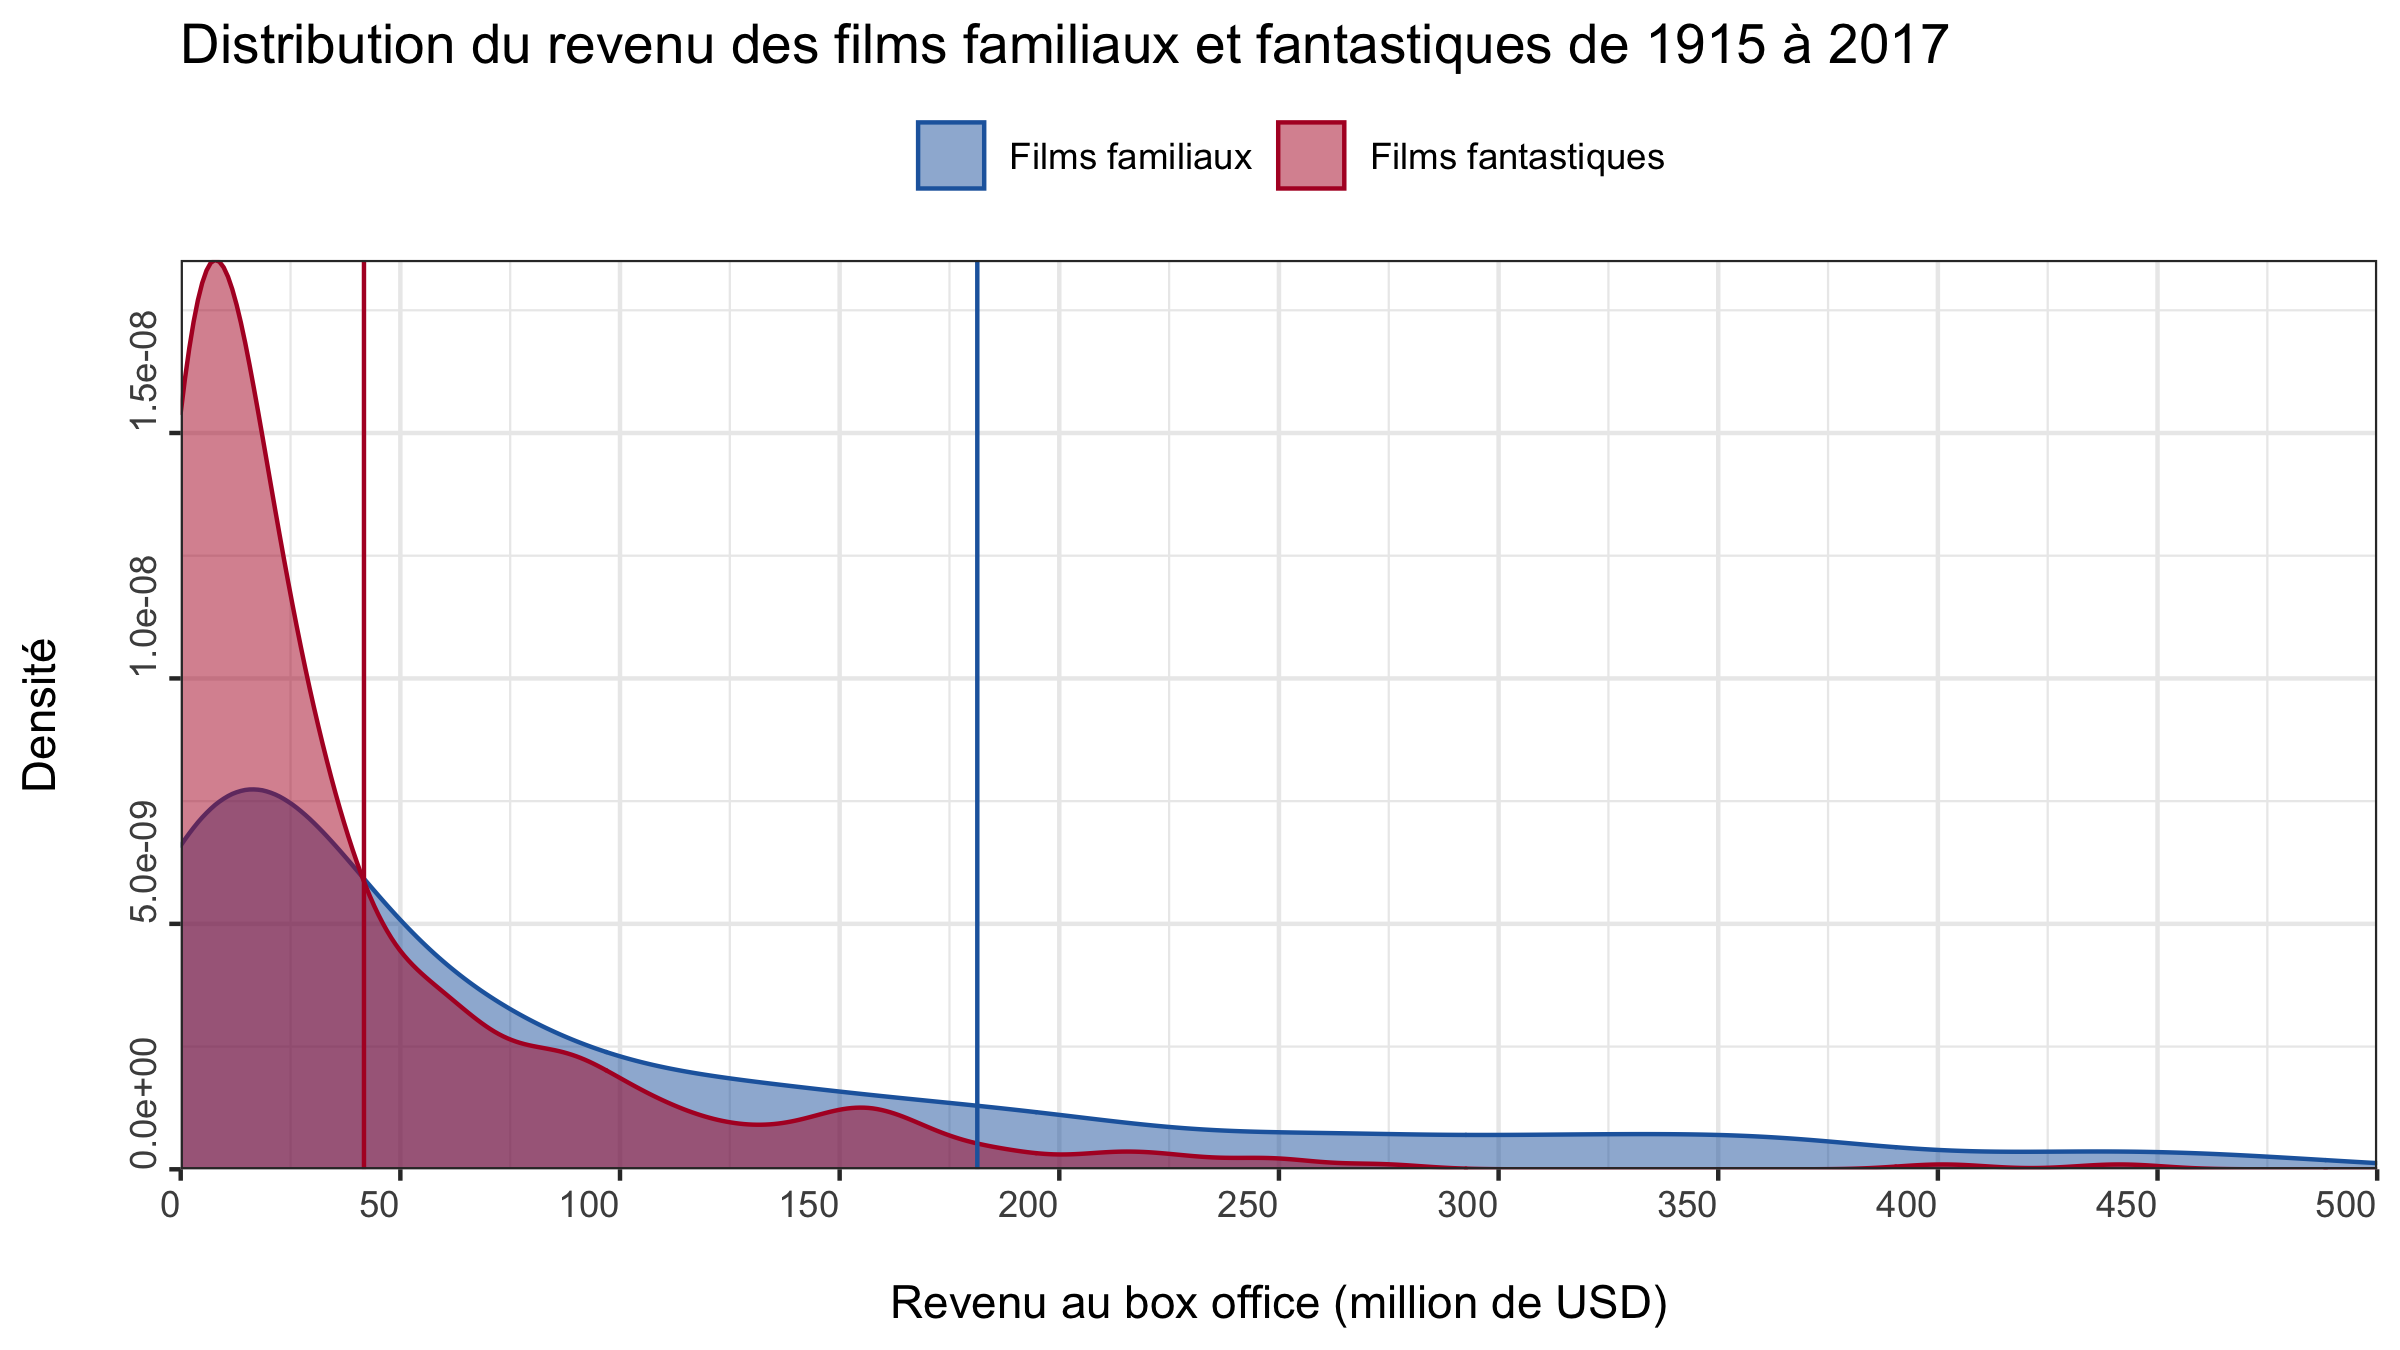
\includegraphics[width=0.98\linewidth]{_graphs/revenueDistri.png}}
    \caption{Exemple d'un graphique plus avancé}
    \label{revenueDistri}
    \end{figure}
    
     \begin{figure}[H]
    \centering
    \fbox{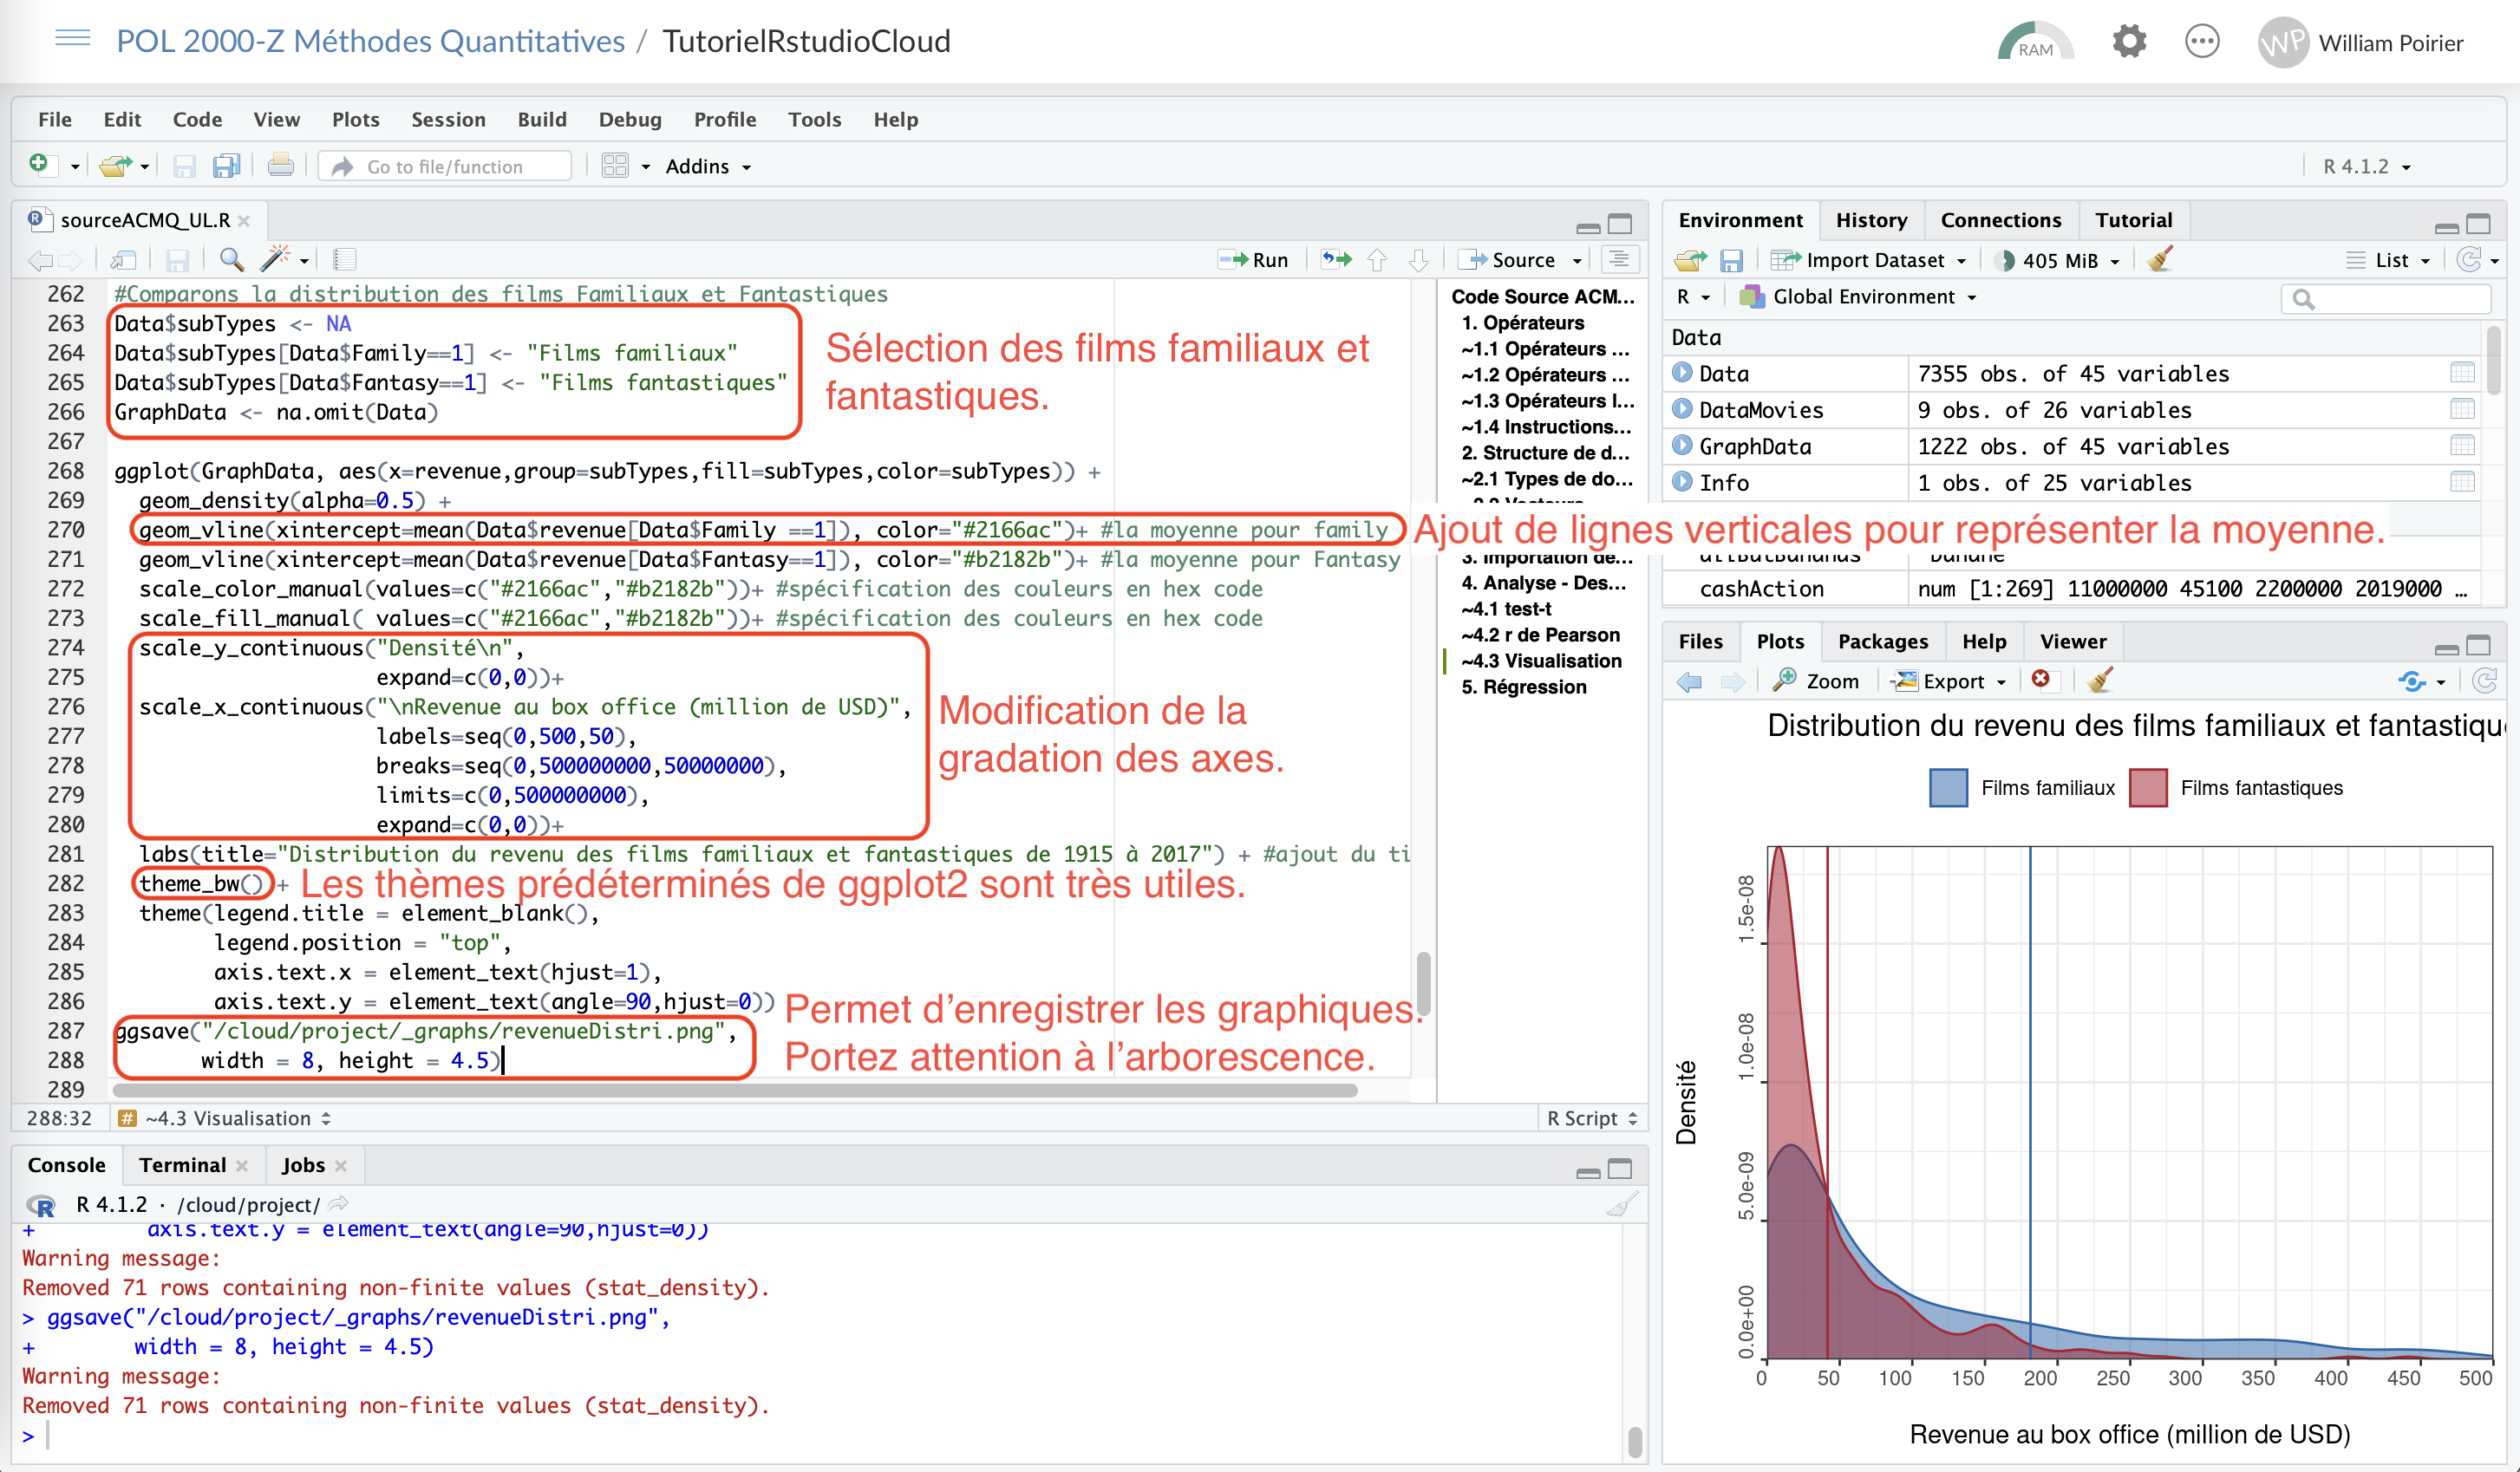
\includegraphics[width=0.98\linewidth]{_graphs/visCode.png}}
    \caption{Code d'un graphique plus avancé}
    \label{visCode}
    \end{figure}
  
 
%\section{Bibliographie}
%\begingroup
%\renewcommand{\section}[2]{}
%\bibliographystyle{apacite}
%\bibliography{mybibfile.bib}
%\vspace{10cm}
%\endgroup

\end{document}